\documentclass[12pt]{article}
\usepackage[utf8]{inputenc}

\usepackage{indentfirst}

\usepackage{gensymb}
\usepackage{titlesec}
\usepackage{graphicx}
\usepackage{booktabs}
\usepackage{wrapfig}
\usepackage{mathtools}
\usepackage{amsmath}
\usepackage[export]{adjustbox}
\usepackage{algorithm}
\usepackage{algpseudocode}
\usepackage{listings}
\usepackage{afterpage}
\usepackage{url}

\usepackage{pgfplotstable}
\pgfplotstableset{
  empty cells with={---},
  every head row/.style={before row=\toprule,after row=\midrule},
  every last row/.style={after row=\bottomrule}
}
\pgfplotsset{compat=1.9}




\usepackage{array,booktabs}

\usepackage{filecontents}
\begin{filecontents*}{data1.txt}
Respuesta Cantidad
1 0
2 0
3 1
4 6
5 6
\end{filecontents*}

\begin{filecontents*}{data2.txt}
Respuesta Cantidad
1 0
2 0
3 2
4 7
5 4
\end{filecontents*}

\setcounter{secnumdepth}{4}
\setcounter{page}{2}
\makeindex
\pagestyle{empty}
\usepackage[left=3cm,top=2.5cm,right=3cm,bottom=3cm]{geometry} %margenes supuestamente
\begin{document}
\null\newpage
\afterpage{\null\newpage}
%titlepage
\thispagestyle{empty}
\begin{center}
\begin{minipage}{0.75\linewidth}
    \centering
%University logo
    
\includegraphics[width=0.3\linewidth]{logofing.png}
    \\Instituto de Computación 
    \\Facultad de Ingeniería Universidad de la República
	\\Montevideo – Uruguay\\
    \vspace{1cm}
%Thesis title
    {\uppercase{\Large Visualización Estereoscópica de Ecuaciones Implícitas\par}}
    \vspace{3cm}
%Author's name
    {\Large Guillermo Báez\\Pablo Coore\par}
    \vspace{1cm}
    Tutor: Eduardo Fernández\\
    \vspace{2cm}
%Degree
    {\Large Proyecto de Grado\par}
    \vspace{3cm}
%Date
    {\Large Agosto 2016}
\end{minipage}
\end{center}


\pagestyle{plain}
\renewcommand{\figurename}{Figura}
\renewcommand{\tablename}{Tabla}
\renewcommand{\contentsname}{Índice}

\section*{Resumen}
\noindent La visualización espacial de ecuaciones es una tarea compleja para estudiantes en todas las etapas de la formación académica. Gran parte del análisis matemático está dedicado a determinar las principales características de las  funciones matemáticas, como punto de partida para lograr su comprensión y entendimiento.

La propuesta de este trabajo consiste en implementar un programa que permita la visualización de ecuaciones implícitas, utilizando tecnologías gráficas relacionadas con la visión estereoscópica.  Ésto  busca acercar al estudiante los componentes estéticos y visuales de las matemáticas. Además se quiere obtener una experiencia de realidad virtual agradable al usuario.

En el marco de este proyecto, se concluyó que los algoritmos basados en la generación de mallas son más adecuados para la visualización estereoscópica debido a que tienen un mejor tiempo de respuesta cuando se actualiza la posición de la cámara.

Se cuenta con una aplicación web\footnote{El código fuente se encuentra disponible en \cite{nuestrocodigo} y se puede acceder a la aplicación en \cite{nuestrositio}}, que funciona  tanto en PC como en celulares,  compatible con Oculus Rift (DK1, DK2 y Consumer Version) si se utiliza el navegador Firefox Nightly, y con Google Cardboard en celulares.
\\
\\
\\
\\
\textbf{Palabras clave:} \textit{Oculus Rift, ambiente virtual inmersivo, visualización de ecuaciones} 


\clearpage
\null\newpage
\tableofcontents
\clearpage
\null\newpage
\section{Introducción}

\subsection{Definición del problema y motivación}
\noindent La visualización espacial de curvas y superficies matemáticas es un reto importante para estudiantes y docentes. Gran parte del análisis matemático está dedicado a determinar las principales características, puntos singulares, pendientes, concavidades y demás características de las  funciones matemáticas, como punto de partida para lograr su comprensión y entendimiento.

En los últimos años se han desarrollado paquetes de software que facilitan la visualización computacional de diversos tipos de ecuaciones. Los paquetes de cálculo científico poseen herramientas de visualización poderosas que hacen posible graficar de forma intuitiva un volumen importante de información compleja\footnote{Por ejemplo Gnuplot es una herramienta libre ampliamente utilizada en el ámbito científico para la visualización de funciones matemáticas y se puede encontrar en \cite{gnuplot}.}.  

En el área de la educación actualmente hay experiencias exitosas, como SURFER\cite{surfer}, 3DXplorMath\cite{dxplormath}, entre otros, que permiten al estudiante introducirse en el mundo de la abstracción geométrica. Además, la visualización de superficies y curvas tridimensionales es ampliamente utilizada en varias disciplinas para la visualización de datos: química, geofísica, meteorología y dinámica de los fluidos, permitiéndo a los ingenieros estudiar características de los mismos mediante simulaciones. Por ejemplo, se puede estudiar el flujo del viento a través de un modelo por computadora de una ala de avión \cite{aircraftwing}, también se pueden utilizar este tipo de técnicas para la visualización de pisos en videojuegos\cite{realtimerendering}\cite{engine}.

En este contexto, se quieren explorar las posibilidades de desarrollar una aplicación donde sea posible visualizar de forma estereoscópica e interactiva (en tiempo real) curvas y superficies matemáticas. Para ello la idea es considerar el uso del dispositivo de visualización Oculus Rift, y aprovechar las capacidades gráficas de las GPU.
\subsection{Objetivos}
\begin{itemize}
\item Desarrollar una aplicación para visualizar ecuaciones algebraicas de forma estereoscópica y en tiempo real.
\item Aprender a utilizar el dispositivo Oculus para la visualización estereoscópica. 
\item Incorporar nuevas facilidades de construcción de superficies, como el uso de operadores booleanos (Geometría Sólida Constructiva). 
\item Estudiar y desarrollar formas interesantes de visualización y recorrido de las superficies.
\item Que la aplicación desarrollada esté disponible para su compilación y ejecución por terceros. 
\end{itemize}
\subsection{Resultados Esperados}
\begin{itemize}
\item Un sitio web desde donde se describan las principales características del software y se tenga acceso al paquete desarrollado para su instalación en equipos de terceros. 
\item Un póster con las principales características del proyecto, para su presentación en actividades académicas.
\end{itemize}
\clearpage
\section{Estado del Arte}
\noindent En esta sección se hará una breve introducción a una serie de conceptos y tecnologías que son la base del proyecto. En la primer sección se definirán los distintos tipos de superficies, como base para explicar en la siguiente sección, dos técnicas para la visualización de un tipo de superficie en particular. 

A continuación se presentará una serie de programas utilizados con el fin de visualizar superficies, así como un breve análisis de los mismos. A su vez se describirá el fenómeno de Virtual Reality Sickness (VRS) que se puede experimentar cuando se presentan determinadas condiciones a la hora de estar trabajando con visualización estereoscópica.

Luego se presentarán una serie de conceptos y hardware utilizados actualmente en la visualización estereoscópica. Además, se listarán varios paquetes de software que fueron utilizados en la realización de la aplicación obtenida como resultado del proyecto.
\subsection{Tipos de superficies}
Una superficie implícita es una superficie en el espacio euclidiano definida por una ecuación $F (x, y, z) =  F(p) = 0$.  Es decir, los  puntos $ p \in {\rm I\!R} ^3$ son parte de la superficie~$ \iff F(p) = 0$ \cite{realtimerendering}.En otras palabras, una superficie implícita es el conjunto de puntos a los cuales aplicarle una función de 3 variables da cero. 

La gráfica de una función 3D se describe generalmente por una ecuación del tipo $z = f (x, y)$ y se denomina  representación explícita\cite{implicitas}\cite{realtimerendering}. La tercera descripción esencial de una superficie es la paramétrica: $(x(s, t), y (s, t), z (s, t))$, donde las coordenadas de los puntos $x$, $y$, $z$ son representadas por tres funciones $x(s, t), y(s, t) , z(s, t)$ dependiendo de los parámetros que tienen en común ($s$ y $t$). En la Figura \ref{ejemplosFiguras} se aprecian dos ejemplos, a la izquierda un tetraedro, y a la derecha ``la copa de vino" que es una superficie de revolución.
\begin{figure}[ht]
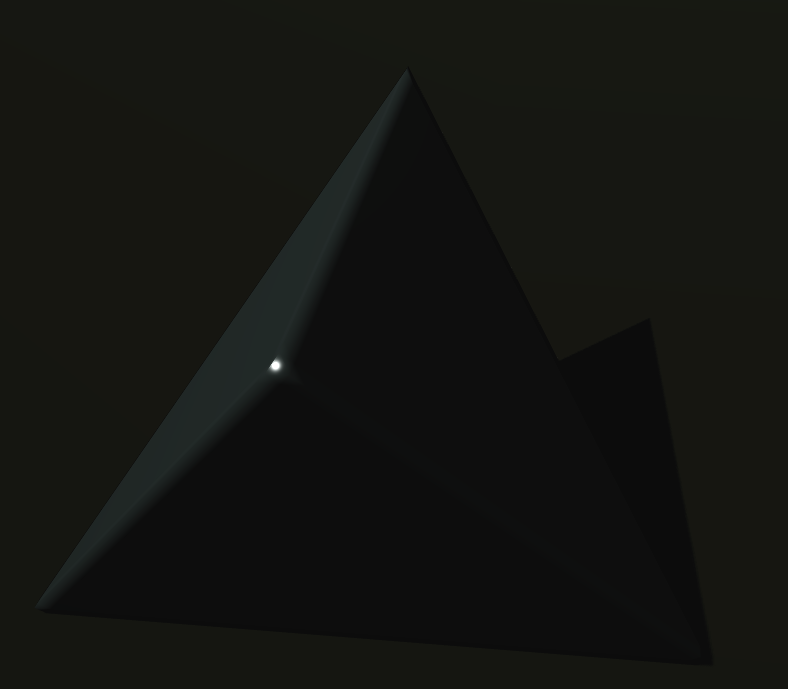
\includegraphics[width =0.45\linewidth]{tetraedro.png}
\hfill
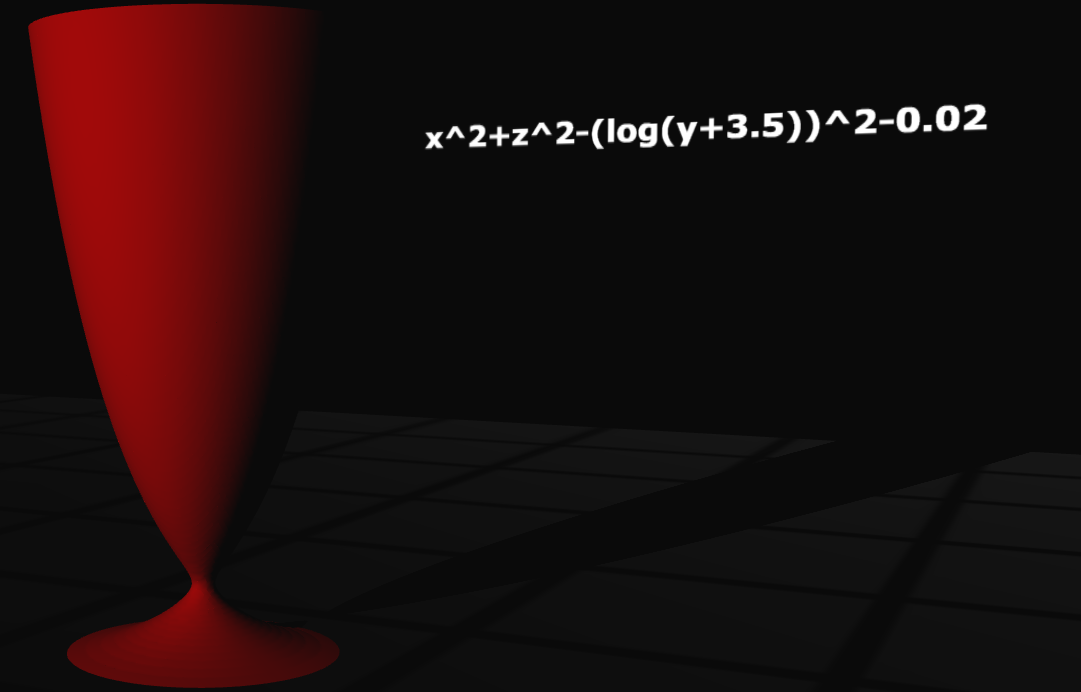
\includegraphics[width =0.45\linewidth]{copa.png}
\caption{ Un tetraedro y una superficie de revolución (``la copa de vino") generados con la aplicación desarrollada.}
\label{ejemplosFiguras}
\end{figure}

Para un plano, una esfera y un toro existen representaciones paramétricas simples. Esto no es cierto para todos los casos de superficies implícitas.

El teorema de la función implícita\footnote{Para más información sobre este teorema ver el anexo A.} describe las condiciones bajo las cuales una ecuación $F (x, y, z) = 0$ se puede resolver localmente para $x$, $y$ o $z$. Pero en general la solución no es factible. Este teorema es clave para el cálculo de características geométricas esenciales de una superficie: planos tangentes, la superficie normales, curvaturas.

Si $F (x, y, z)$ es un polinomio en $x$, $y$ y $z$, la superficie se llama algebraica,  por ejemplo, la superficie correspondiente a la copa de vino no es algebraica.

\subsection{Técnicas para visualización de superficies implícitas}
\noindent En este punto se presentan de forma breve dos técnicas para la visualización de superficies implícitas, así como un breve análisis de sus ventajas y desventajas.
\subsubsection{Ray casting}
\noindent La técnica de ray casting consiste en trazar rayos de modo de simular ciertos aspectos geométricos de la luz y cómo son percibidos por las personas (ver Figura \ref{raycasting}). La forma de hacerlo es lanzando rayos desde un punto (los rayos tienen un origen común si se quiere que la imagen sea una proyección perspectiva, de lo contrario tienen como origen un píxel de la grilla y poseen la misma dirección), el cual representa el ojo o cámara, de manera que atraviese un píxel de la imagen que se desea generar y luego se detecta con qué superficie interseca. Una vez que se obtiene el primer punto de intersección del rayo se le da un color al píxel atravesado utilizando distintas técnicas de sombreado.
%\clearpage
\begin{figure}[h!]
\includegraphics[width=0.65\textwidth,center]{raycasting.png}
\caption{Ilustración del funcionamiento de ray casting.}
\label{raycasting}
\end{figure}

Cada rayo se escribe $\textbf{r}(t)= o +td$ siendo $o$ el origen (el ojo) y $d$ la dirección entre el origen y el píxel que se desea calcular. Si tenemos la función implícita $F(p)=0$, donde $p \in {\rm I\!R} ^3 $, entonces para detectar la intersección de un rayo con una ecuación implícita basta con resolver $F(\textbf{r}(t))=0$.
A continuación, a modo de ejemplo, presentamos cómo obtener la intersección entre un rayo y una esfera de forma analítica\cite{realtimerendering}.

Sea la superficie implícita $F(p)=\lVert p -c \rVert - r = 0$, donde $c$ es el centro de la esfera y $r$ es el radio.
\begin{center}
$ F(\textbf{r}(t))= 0$
\\$ \iff$
\\$ \lVert \textbf{r}(t) -c \rVert - r = 0$
\\$ \iff$
\\$ \lVert \textbf{r}(t) -c \rVert = r$
\\ $\iff$
\\ $(o+td -c).(o+td -c) = r^2 $ 
\\ $\iff$
\\$t^2(d.d) + 2t(d.(o-c)) + (o-c).(o-c) - r^2=0$
\\ $\iff$ (\footnote{En este paso se asume que el vector de dirección $d$ se encuentra normalizado})
\\$t^2 + 2t(d.(o-c)) + (o-c).(o-c) - r^2=0$
\end{center}

Utilizando Báscara se obtienen los dos valores posibles de $t$. Notar que si $d$ está normalizado $t$ es la distancia entre $o$ y el punto de intersección. $\lVert o + td - o \rVert = \lVert td\rVert = |t|\lVert d \rVert$.

Para obtener un visualizador de ecuaciones implícitas el reto está en encontrar un método para hallar las raíces de la ecuación $F(\textbf{r}(t))=0$ para toda función implícita. El desafío es aún más complejo si se desea lograr que éste funcione en tiempo real, ya que para cada frame se deberán realizar cientos de intersecciones entre rayos y la función.  
\subsubsection{Meshers}
\noindent Esta técnica consiste en obtener una aproximación poligonal de la geometría, para luego visualizarla utilizando cualquier método de visualización que soporte este tipo de geometría. Una vez realizada la aproximación poligonal ya no es necesario operar con la función para su visualización.

Para realizarla primero se obtiene una aproximación de la función realizando un muestreo de la misma. Una vez que se halla esto se aplica un algoritmo para la obtención de los polígonos (en la Sección 3 se presentan 4, los cuales son Marching Cubes, Marching Tetrahedra, Surface Nets y Dual Contour)\cite{mykola1}\cite{mykola2}.

La principal ventaja de este método sobre ray casting es que una vez generada la aproximación no se debe trabajar más con la ecuación, esto permite que si se trabaja en tiempo real no ocurra que ecuaciones más complejas tengan framerates más bajos. Por este motivo este tipo de método es ideal para aplicaciones en tiempo real, ya que sólo se deben realizar operaciones complejas antes de iniciar la visualización, luego se puede visualizar utilizando por ejemplo la técnica del Z-buffer utilizando APIs como OpenGL o Direct3D.

La principal desventaja es que la figura obtenida es una aproximación poligonal, a diferencia de ray casting que obtiene una imagen con un mayor nivel de similitud respecto a la superficie real\cite{realtimerendering}.

\subsection{Software de representación de superficies implícitas}
\noindent A continuación se presentan 3 programas que son utilizados para la representación de este tipo de superficies.
\subsubsection{SURFER}
\noindent SURFER es una herramienta de Imaginary desarrollada en Java que permite la visualización de superficies implícitas del tipo algebraico. La misma utiliza JavaFX para la interfaz de usuario, y las ecuaciones se muestran utilizando el motor de render JSURFER, el cual es un aplicación basada en ray casting implementado en CPU que utiliza el algoritmo de Descartes para hallar los puntos de intersección de los rayos con las ecuaciones. La aplicación utiliza proyección ortográfica para representar las ecuaciones en el plano.

Esta aplicación se analiza con mayor detenimiento en la Sección 4.
\subsubsection{3d-XplroMath-J}
\noindent Otra aplicación que representa superficies es 3d-XplroMath-J, la cual es una reimplementación de 3d-XplroMath implementada en Java. Esta aplicación no usa ray casting sino que utiliza aproximaciones poligonales. La aplicación fue inicialmente diseñada para utilizar JavaGraphics2D, pero luego se modificó para funcionar con OpenGL. 3D-XplorMath-J utiliza un  renderizador definido por una interfaz, Renderer3D, para extraer sus imágenes. 

OpenGL ofrece la posibilidad de generar dibujos 3D acelerados por hardware, con la posibilidad de gráficos mejorados y una gran aceleración en comparación con la aplicación de dibujo 3D con Graphics2D. OpenGL es implementado en Java utilizando la API JOGL.

Esta aplicación no cuenta con un ingreso de superficies de forma tan amigable como SURFER. Las superficies se muestran de forma estática, y cuando se rotan se muestran en modo wireframe.
\subsubsection{Isosurface}
\noindent Isosurface es una aplicación web que implementa los algoritmos de Marching Cubes, Marching Tetahedra y Naive Surface Nets (los cuales se describen en la Sección 3) en Javascript. La misma muestra algunas superficies de ejemplo, pero no permite introducir ecuaciones ni tiene un menú interactivo que permita modificar las superficies mostradas. Además, la aplicación muestra las superficies de una forma poligonal, resaltando los diferentes polígonos que se utilizan para aproximar la ecuación.  
\subsection{Visión estereoscópica}
\noindent Consiste en la percepción de la profundidad y la estructura de 3 dimensiones utilizando información derivada de los dos ojos. Debido a que los ojos de los seres humanos se encuentran en diferentes posiciones laterales en la cabeza, los resultados de la visión binocular son dos imágenes ligeramente diferentes proyectadas para las retinas de los ojos (ver Figura \ref{disparidades}). Las diferencias están principalmente en la posición horizontal relativa de los objetos en las dos imágenes. Estas diferencias posicionales se conocen como las disparidades horizontales o, más en general, las disparidades binoculares. Las disparidades se procesan en la corteza visual del cerebro para producir la percepción de profundidad\cite{visionest}. 
\begin{figure}[h!]
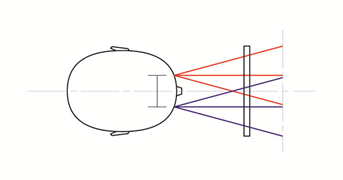
\includegraphics[width =0.7\linewidth, center]{ojos.png}
\caption{Disparidades binoculares.}
\label{disparidades}
\end{figure}

Mientras que las disparidades binoculares están naturalmente presentes durante la visualización de una escena en 3 dimensiones real con dos ojos, las mismas deben ser simuladas mediante la presentación de dos imágenes diferentes por separado a cada ojo utilizando un método llamado estereoscópica. La percepción de la profundidad en tales casos también se refiere como ``profundidad estereoscópica". 

La percepción de la profundidad y la estructura tridimensional  es, sin embargo, posible con la información de un ojo solamente, utilizando las diferencias en el tamaño de objeto y el paralaje de movimiento (diferencias en la imagen de un objeto a través del tiempo con el movimiento observador), aunque la impresión de profundidad en estos casos no es a menudo tan buena como la obtenida de las disparidades binoculares. Por lo tanto, el término estereopsis (o profundidad estereoscópica) también puede referirse específicamente a la impresión única de profundidad asociada con la visión binocular, lo que coloquialmente se conoce como ver ``en 3D".

La estereoscopía es una técnica para crear o mejorar la ilusión de profundidad en una imagen por medio de la estereopsis para la visión binocular. Cualquier imagen estereoscópica se llama un estereograma. 

La mayoría de los métodos estereoscópicos presentan  dos imágenes “movidas” por separado para el ojo izquierdo y derecho del espectador. Estas imágenes de dos dimensiones se combinan entonces en el cerebro para dar la percepción de la profundidad 3D.

Un fenómeno que puede acontecer es virtual reality sickness (VRS, también conocido como cybersickness y como simulator sickness), el cual se produce cuando la exposición a un entorno virtual causa síntomas que son similares a los síntomas de la motion sickness\cite{VRS} (en español el fenómeno es conocido como Cinetosis). Los síntomas más comunes son malestar general, dolor de cabeza, la conciencia del estómago, náuseas, vómitos, palidez, sudoración, fatiga, somnolencia, desorientación y apatía. Otros síntomas incluyen la inestabilidad postural y las arcadas. Este fenómeno tiende a caracterizarse por la desorientación.

Este efecto es diferente a la cinetosis, ya que puede ser causada por la percepción visual inducida de movimiento. No es necesaria que la persona se mueva para sufrir sus síntomas.

La fisiología de la VRS actualmente no está claramente entendida. Afortunadamente, la investigación ha descubierto algunas indicaciones claras de ciertas condiciones que la causan. Parece que las imágenes proyectadas desde la realidad virtual tienen un gran impacto en la enfermedad. La frecuencia de actualización de las imágenes en pantalla a menudo no es lo suficientemente alta cuando se produce la VRS. Debido a que la frecuencia de actualización es más lenta que los procesos cerebrales, causa una descoordinación entre el tipo de procesamiento y la velocidad de actualización, lo que hace que el usuario perciba fallos en la pantalla. Cuando estos dos componentes no coinciden, puede causar al usuario las mismas sensaciones que cuando se experimenta motion sickness.

La resolución sobre la animación también puede hacer que los usuarios experimenten este fenómeno\cite{oculussickness}. Esto puede ser cuando las animaciones son pobres, que  causa otro tipo de discordia entre lo que se espera y lo que realmente está sucediendo en la pantalla. O cuando los gráficos en pantalla no mantienen el ritmo con los movimientos de la cabeza del usuario, desencadenando una forma de motion sickness.
\subsection{Tecnologías existentes para visión estereoscópica}
\noindent En la actualidad está saliendo al mercado una gran serie de dispositivos que aplican los conceptos de la estereoscopía para generar el efecto de estar en un espacio virtual.

Existen varios productos para dispositivos no móviles, por ejemplo  Oculus Rift\cite{oculus}, Playstation VR\cite{psvr} y HTC Vive\cite{htcvive}. A su vez existen varios para dispositivos móviles como  Google Cardboard\cite{cardboard} y  Samsung Gear VR\cite{samsungvr}, estos dispositivos requieren de celulares para funcionar (utilizándolos como pantalla y como sensor de rotación).

Lo que tienen en común estos dispositivos es que todos cuentan con una pantalla, dos cristales y sensores para reconocer los movimientos de la cabeza \footnote{Particularmente rotaciones, aunque actualmente algunos de ellos utilizan cámaras de forma de poder reconocer si se mueve la cabeza hacia adelante o hacia atrás por medio del traqueo de una luz}.

La resolución de las pantallas, así como su velocidad de refresco varían según el dispositivo. Éste es un aspecto muy importante, ya que la calidad final de la experiencia se verá muy afectada por este factor, debido a que, si la imagen se encuentra muy pixelada, la experiencia no será agradable, y si la velocidad de refresco no es buena, se podrían producir mareos y náuseas al usuario.

Los sensores son utilizados principalmente para permitir al usuario mirar hacia “los costados” de forma de explorar la escena, generando un mayor nivel de inmersión.

Los cristales de los dispositivos de visión estereoscópica proveen un campo visual (FOV) muy amplio, permitiendo una mayor inmersión, pero para lograrlo generan una distorsión\cite{oculusrendering} en la imagen como muestra la siguiente figura. Este tipo de distorsión se conoce como  distorsión de acerico (pincushion distortion en inglés), lo que provocaría, que si no se utiliza ningún tipo de corrección sobre las imágenes que se le envían al dispositivo, todo se vería distorsionado como se ve en la Figura \ref{dist}.
\begin{figure}[h!]
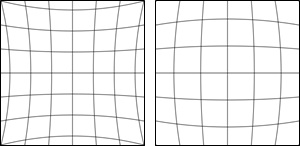
\includegraphics[width =0.6\linewidth, center]{ace-bar.png}
\caption{ A la izquierda se puede apreciar la distorsión de acerico y a la derecha la de barril.}
\label{dist}
\end{figure}

Para corregir la deformación producida se utiliza la distorsión de barril (barrel distortion en inglés), la cual genera el efecto inverso (como se puede ver en la imagen) y provoca que el usuario que utiliza los lentes no se de cuenta de la curvatura de los cristales, pero siendo beneficiado por la inmersión generada por el gran campo visual\cite{oculusrendering}. 

A continuación, en la Figura \ref{lenna}, mostramos una imagen que es comúnmente utilizada a la hora de probar algoritmos sobre imágenes, en las tres formas, la primera es como se ve normalmente, la del medio es si se le aplica una distorsión de barrido y la última es como se visualiza luego de una distorsión de acerico.
\begin{figure}[h!]
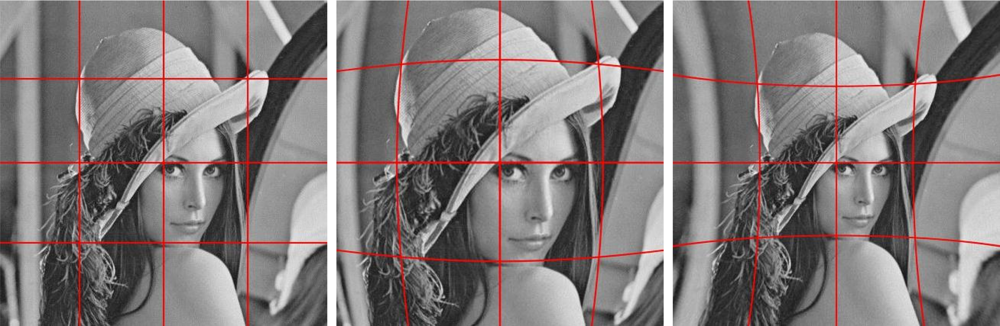
\includegraphics[width=0.8\textwidth, center]{imagen_clasica.png}
\caption{Se muestra la imagen sin distorsionar y luego de aplicar cada una de las distorsiones mencionadas.}
\label{lenna}
\end{figure}

\subsubsection{ Oculus Rift}
\noindent El Oculus Rift es un casco de realidad virtual desarrollado y fabricado por Oculus VR, lanzado al mercado en marzo de 2016. Antes del lanzamiento de la versión para el consumidor se lanzaron varias para los desarrolladores, a continuación se presentan algunas de ellas\cite{oculus}.
\paragraph{Development kit 1}
La versión DK1 (Development Kit 1) utiliza una pantalla de 7 pulgadas (18 cm) con un tiempo de refresco de píxeles significativamente menor que el prototipo original, lo que reduce la latencia y el motion blur al girar la cabeza rápidamente. El “relleno de píxeles” también fue mejorado, lo que  implica que el usuario no nota con tanta facilidad los píxeles en pantalla. El LCD es más brillante y la profundidad de color es de 24 bits por píxel. La pantalla tiene una resolución de 1280x800 (en total, 640x800 por ojo) y posee una velocidad de refresco de 60Hz. El dispositivo se puede apreciar en la Figura \ref{dk1}.
\begin{figure}[h!]
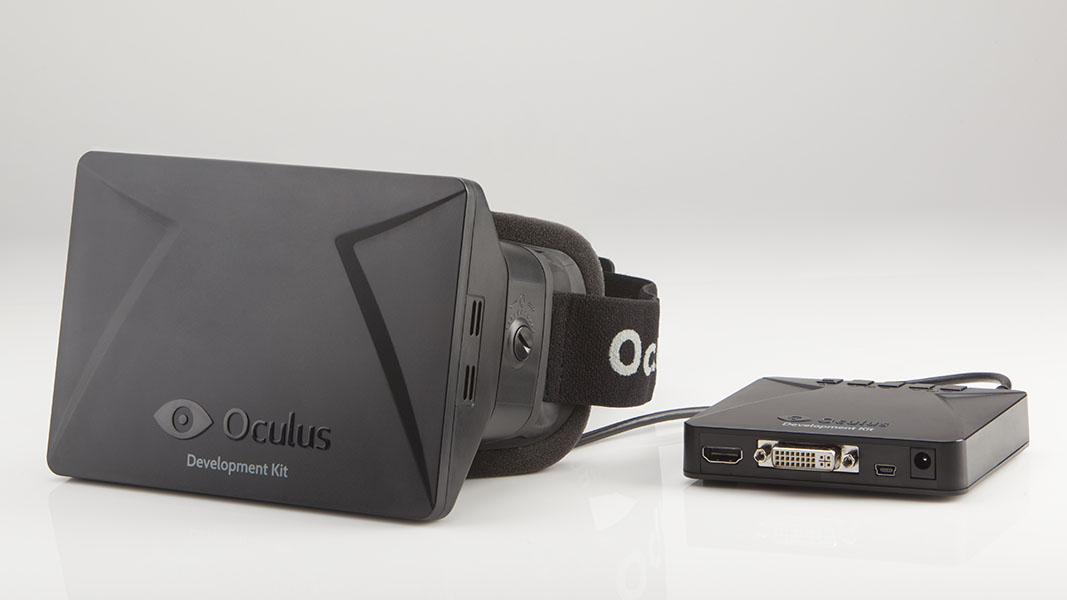
\includegraphics[width=0.8\textwidth,center]{dk1.jpg}
\caption{Oculus Rift Development Kit 1.}
\label{dk1}
\end{figure}

Esta versión cuenta con una pequeña “caja de control” donde se conecta lo necesario, y para su funcionamiento además de ser conectado a la computadora por medio de un cable USB y un cable de video (por ejemplo HDMI), debe ser conectado a la corriente. 
\paragraph{Development kit 2}

Oculus comenzó a distribuir a los clientes que habían reservado DK2 ( Development Kit 2) en julio de 2014. Esta nueva versión ofrece varias mejoras clave en relación al primer kit de desarrollo, tales como tener una mayor resolución (960x1080 por ojo, es decir 1920x1080 en total, la resolución que se conoce como FullHD), una pantalla OLED, una mayor frecuencia de refresco de 75 Hz, el seguimiento de posición a través de un sensor externo al Rift, un cable desmontable,  la omisión de la necesidad de la caja de control externa y finalmente ya no es necesario conectarlo a la corriente (ver Figura \ref{dk2}).
\begin{figure}[h!]
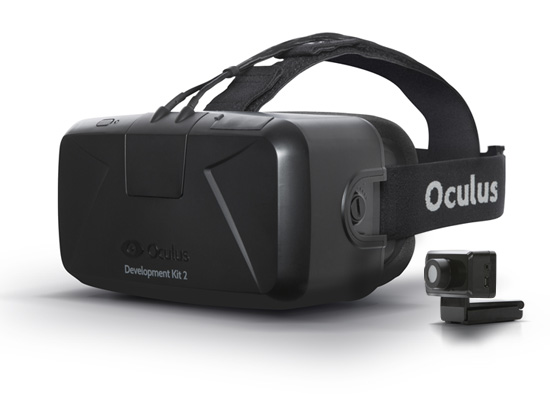
\includegraphics[width=0.8\textwidth,center]{dk2.jpg}
\caption{Oculus Rift Development Kit 2.}
\label{dk2}
\end{figure}

La pantalla pasó de ser de 7 a 5.7 pulgadas. Una exploración del dispositivo, reveló que incorpora un smartphone Samsung Galaxy Note 3 modificado como pantalla.
\paragraph{Consumer version}
La versión que fue lanzada para el público en general tiene una pantalla OLED de 1080x1200 por ojo, una tasa de refresco de 90 Hz y 110 $^{\circ}$ campo de visión. Posee auriculares integrados que proporcionan un sonido con efecto 3D, efecto de rotación y de seguimiento de posición. El sistema de seguimiento de posición, denominado ``Constellation", se realiza mediante un sensor IR LED USB que se encuentra apuntando hacia el dispositivo Rift, que normalmente se encuentra en el escritorio del usuario, e identifica toda la habitación con luces infrarrojas y LED, lo que crea un espacio 3D, permitiendo al usuario utilizar el dispositivo mientras se está sentado, de pie o caminar alrededor de la misma habitación. Esta versión se aprecia en la Figura \ref{cv}.
\clearpage
\begin{figure}[h!]
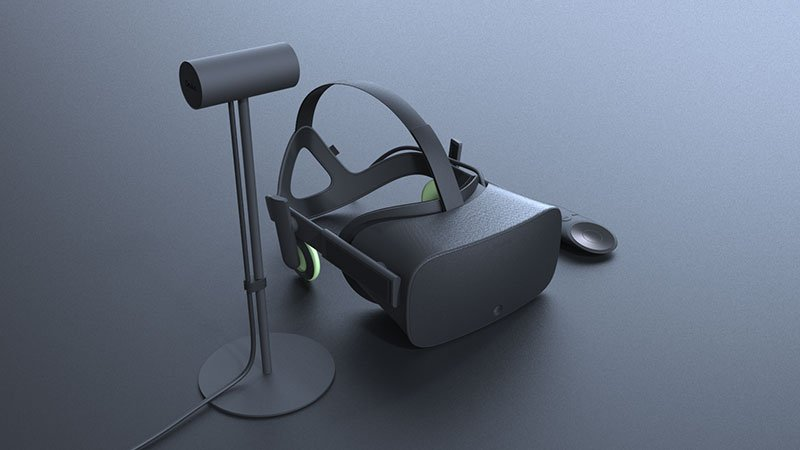
\includegraphics[width=0.8\textwidth,center]{cv.jpg}
\caption{Oculus Rift Consumer Version.}
\label{cv}
\end{figure}

En la Tabla \ref{tablaOR} se muestra una comparación entre las tres versiones de Oculus Rift que se mencionaron anteriormente. En la misma se puede apreciar como han ido mejorando las sucesivas versiones, particularmente en cuanto a la resolución y a la tasa de refresco.
\begin{table}[h!]
  \centering
  \begin{tabular}{cccc}
    \toprule
     & DK1 & DK2 & CV\\
    \midrule
    OLED & No & Sí & Sí\\
    Resolución & 1280x800 & 1920x1080 & 2160x1200 \\
    Frecuencia de refresco de imagen & 60Hz & 75Hz & 90Hz\\
    Campo Visual & 110 grados & 100 grados & 110 grados\\
    Acelerómetro, giroscopio, magnetómetro & Sí & Sí & Sí\\  
    Frecuencia de refresco del acelerómetro & 1000Hz& 1000Hz & 1000Hz\\
    Traqueo orientacional & Sí & Sí & Sí\\ 
    Traqueo posicional & No & Sí & Sí\\
    Caja de control externa & Sí & No & No\\
    \bottomrule
  \end{tabular}
  \caption{Comparación entre las versiones de Oculus Rift.}
\label{tablaOR}
\end{table}
\clearpage
\subsubsection{HTC Vive}
\noindent Este dispositivo posee una resolución de 2160 x 1200, un campo visual de 110 grados y una tasa de refresco de 90 Hz. Es comercializado con dos controles que rastrean el movimiento de las manos para poder brindar experiencias más inmersivas\cite{htcvive}. El mismo se puede ver en la Figura \ref{htcV}.
\begin{figure}[h!]
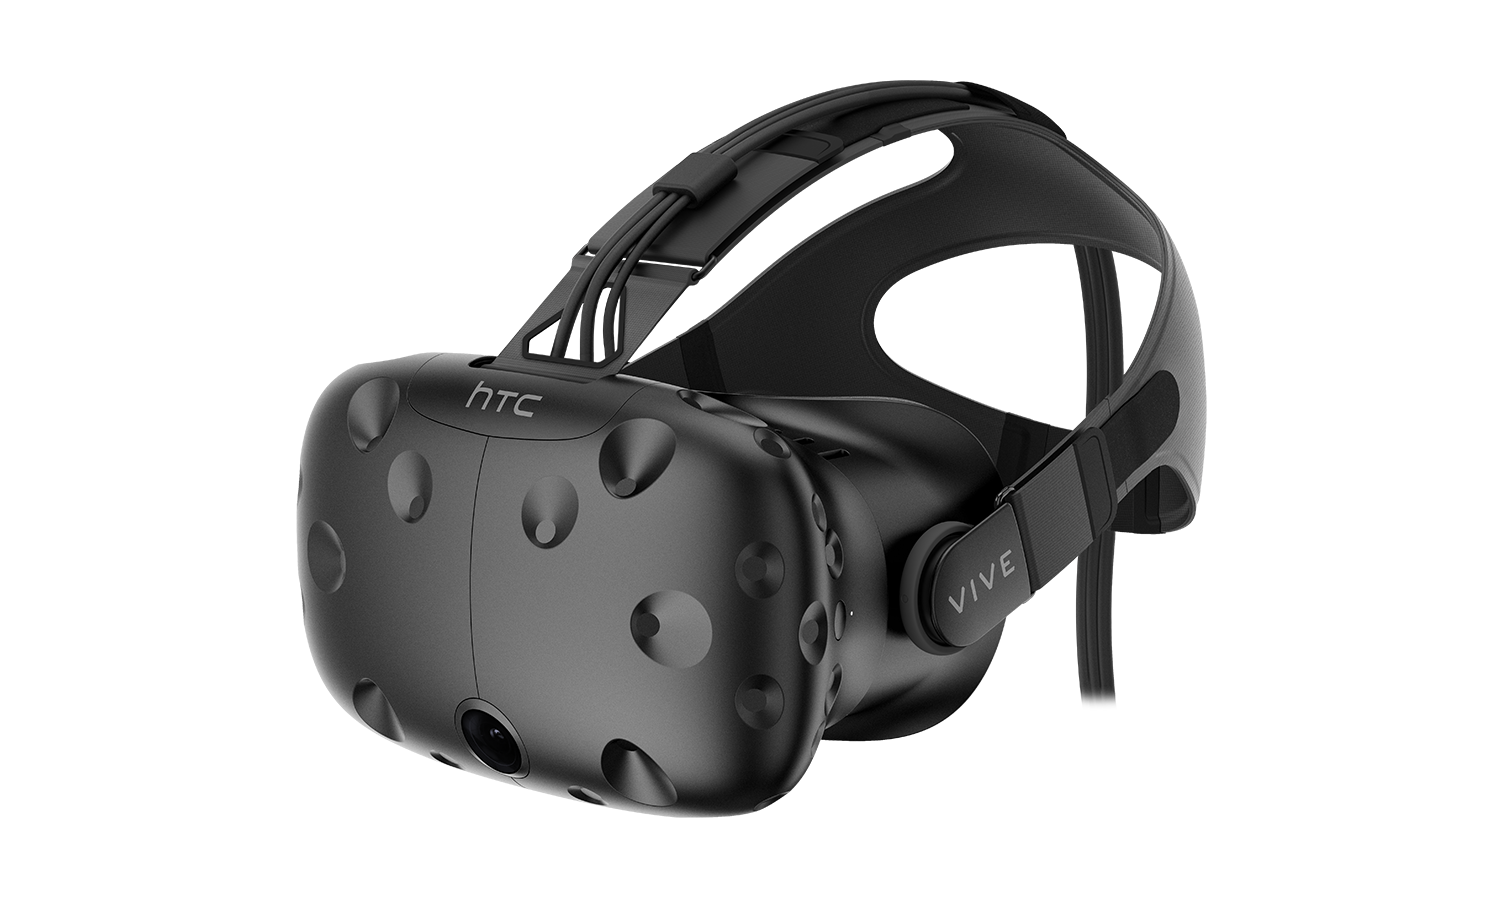
\includegraphics[width=0.8\textwidth,center]{htc.png}
\caption{HTC Vive.}
\label{htcV}
\end{figure}
\subsubsection{PlaystationVR}
\noindent Es el dispositivo para la visión estereoscópica de Sony para ser utilizado con su consola de videojuegos PlaySation 4. A diferencia de los otros equipos, no ha sido lanzado al mercado, se prevee que sea lanzado en octubre del presente año. Por más que no se encuentre disponible, la empresa anunció que no será compatible con PC. En la Figura \ref{psvr} se puede apreciar cómo lucirá.

Posee una pantalla de 5,7 pulgadas, y una resolución de 1920x1080, es decir 960x1080 por ojo. La velocidad de refresco es de 90 Hz o 120 Hz y tiene un campo visual de 100 grados\cite{psvrspecs}.
\clearpage
\begin{figure}[h!]
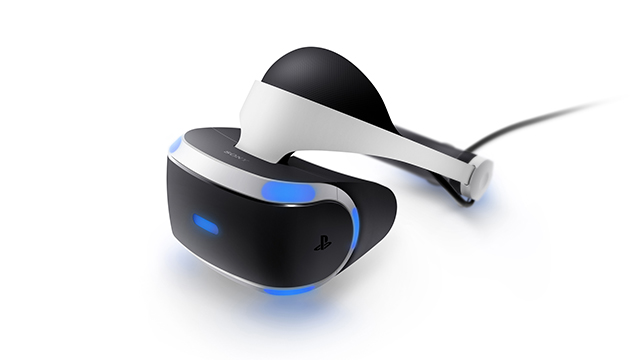
\includegraphics[width=0.8\textwidth,center]{psvr.jpg}
\caption{PlaystationVR.}
\label{psvr}
\end{figure}
\subsubsection{Google Cardboard}
\noindent Es una plataforma de realidad virtual desarrollada por Google\cite{cardboard} para su uso con un visor plegable y teléfono inteligente. Llamado así por su visor de cartón plegable (ver Figura \ref{card}), pretende ser un sistema de bajo costo para estimular el interés y el desarrollo de aplicaciones de realidad virtual. Los usuarios pueden construir su propio visor de componentes simples y de bajo coste utilizando las especificaciones publicadas por Google, o comprar una de las versiones pre-fabricadas. Para utilizarlo es necesario  la colocación de un dispositivo móvil en la parte posterior de la carcasa y se  visualiza a través de los lentes en la parte delantera.
\begin{figure}[h!]
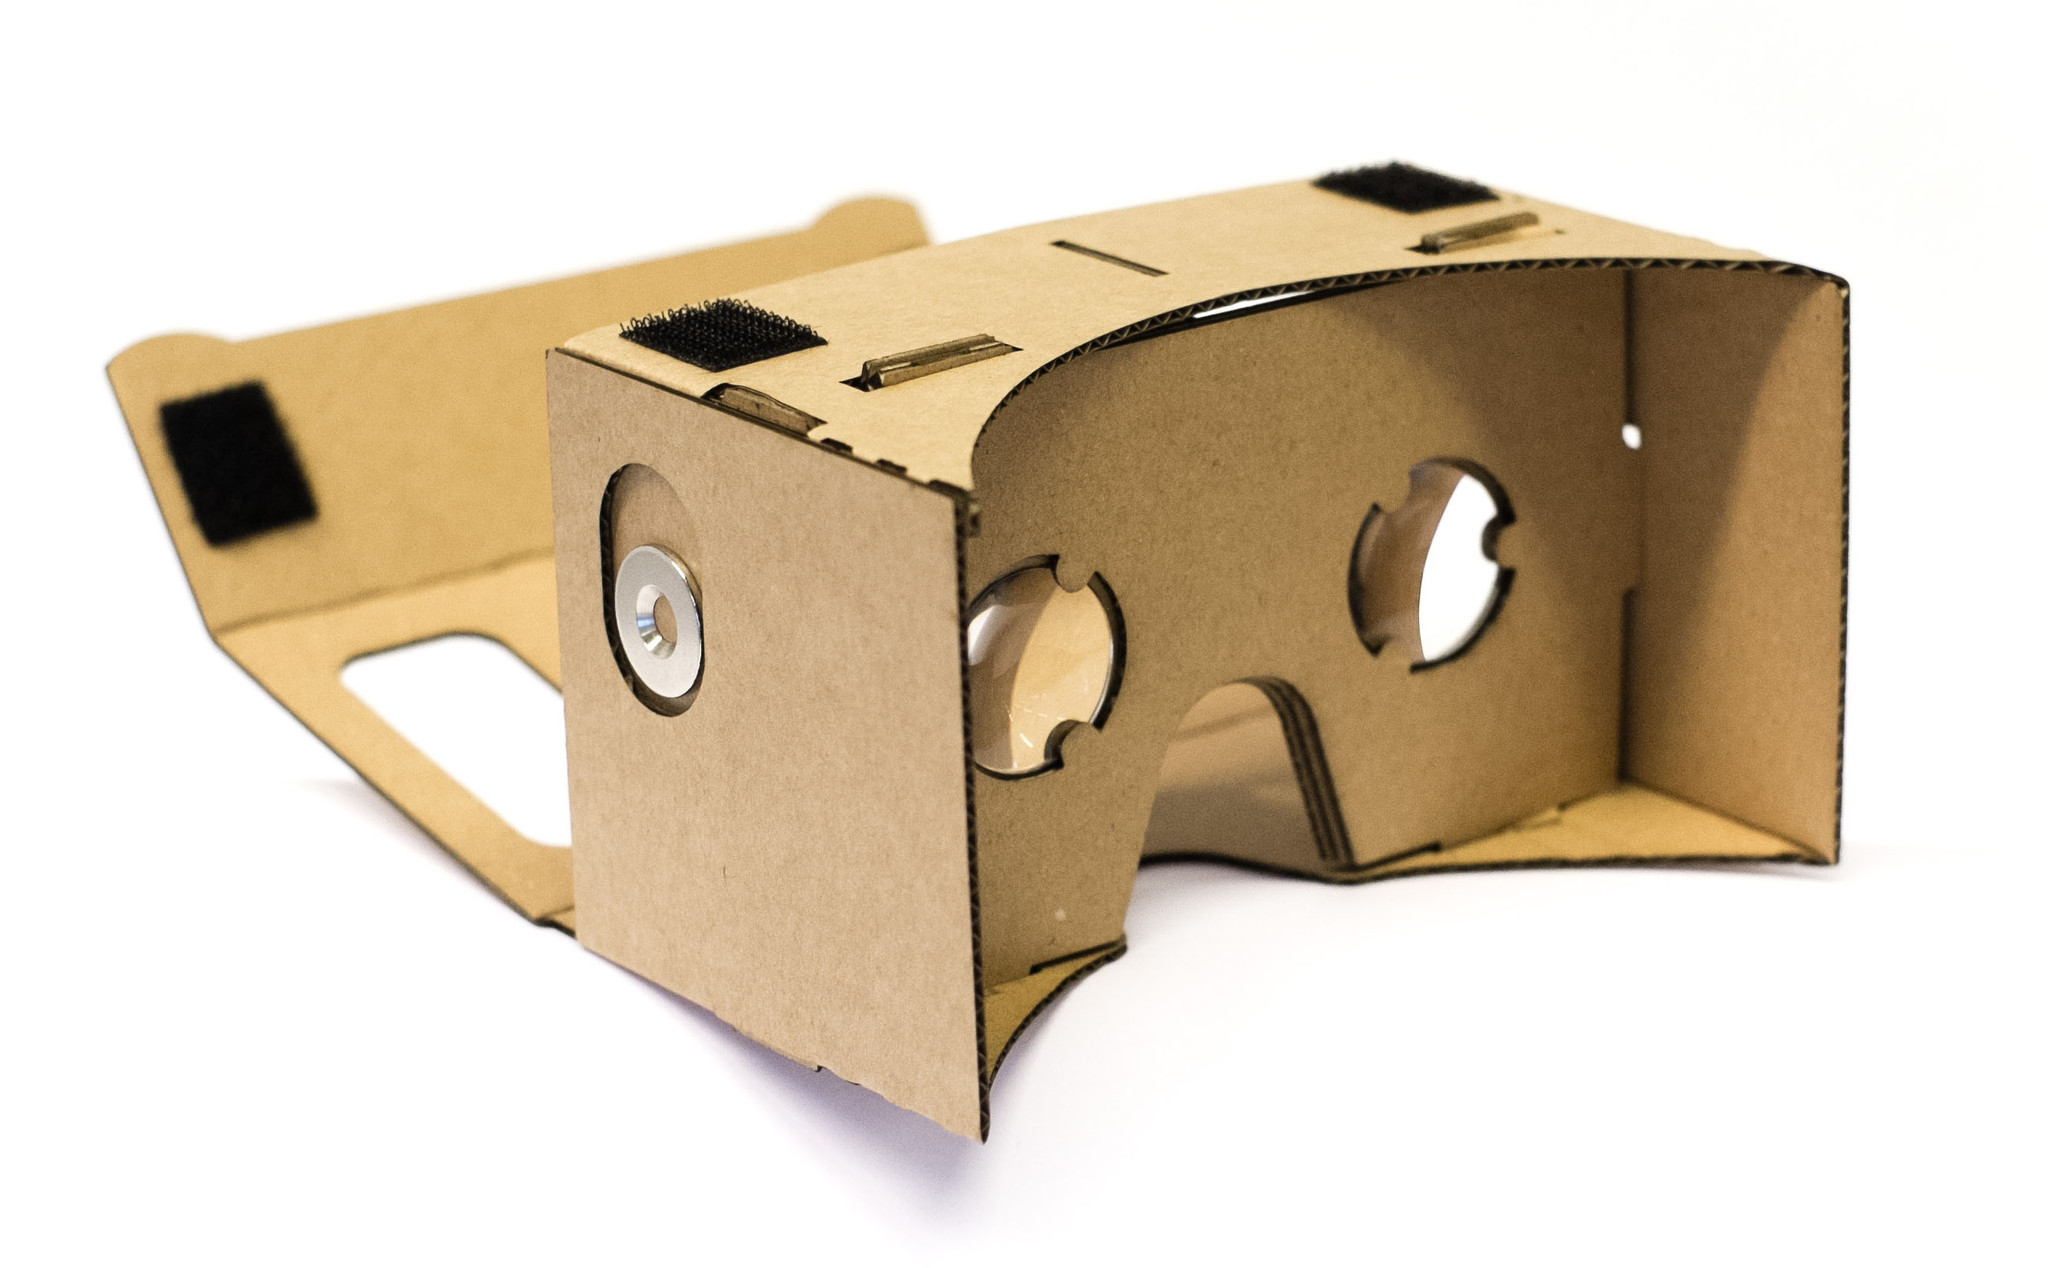
\includegraphics[width=0.7\textwidth,center]{google_cardboard.jpg}
\caption{Ejemplo de Google Cardboard.}
\label{card}
\end{figure}

Fue introducido en la Google I/O 2014, donde un visualizador Google Cardboard fue regalado a todos los asistentes. El kit de desarrollo (SDK) está disponible para los sistemas operativos Android e iOS, mientras que una separada VR Ver SDK permite a los desarrolladores integrar contenidos de RV en la web, así como en sus aplicaciones móviles. 
\subsubsection{Samsung Gear VR}
\noindent Al igual que Google Cardboard, requiere un celular para su funcionamiento. En este caso el teléfono debe ser un Samsung Galaxy S6, Samsung Galaxy Note5 o Samsung Galaxy S7\cite{samsungvr}. Lo que lo hace más restrictivo que Google Cardboard.

Este dispositivo (ver Figura \ref{sgvr}) fue desarrollado en conjunto con Oculus\cite{samsungvr}.
\begin{figure}[h!]
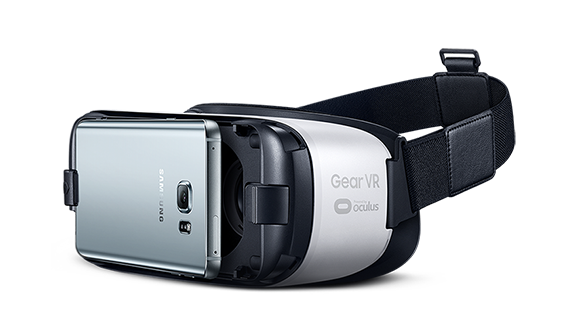
\includegraphics[width=0.8\textwidth,center]{samsungvr.png}
\caption{Samsung Gear VR.}
\label{sgvr}
\end{figure}

\subsection{Otros paquetes gráficos}
\noindent En esta sección se presentan varios paquetes gráficos que fueron utilizados en el desarrollo de la aplicación final.
\subsubsection{WebGL}
\noindent WebGL (Web Graphics Library) es una API de JavaScript para la representación  de gráficos 3D y 2D  interactivos dentro de cualquier navegador web compatible sin el uso de plug-ins. WebGL está integrado en la mayoría de los navegadores que permiten acelerado por la GPU, el uso de la física y de procesamiento de imágenes. Los elementos de WebGL se pueden mezclar con otros elementos HTML y componerse con otras partes de la página. Los programas que utilizan WebGL tienen código escrito en JavaScript y  código de sombreado que se ejecuta en la unidad de procesamiento gráfico de un ordenador (GPU). 
\subsubsection{THREEJS}
\noindent THREEJS es una biblioteca liviana\cite{three} de JavaScript para trabajar con 3D, la cual puede ser utilizada con un canvas de HTML5 o con WebGL. Fue creada en 2010, aunque originalmente fue desarrollada en ActionScript, pero rápidamente fue traducida a JavaScript\footnote{El código fuente se puede obtener en \cite{codigothree}}.

Posee como característica principal que es compatible con todos los navegadores compatibles con WebGL, esto permite que las aplicaciones desarrolladas con él sean posibles de ejecutar en la gran mayoría de los navegadores modernos.

Además la biblioteca permite utilizar WebGL de forma más sencilla y accesible, ya que trae ciertas funcionalidades ya implementadas.
\subsubsection{MozVR}
\noindent Es el proyecto de Mozilla para agregar la posibilidad de usar realidad virtual en páginas web (WebVR)\cite{mozvr}. Permite que versiones experimentales de Firefox sean compatibles con Oculus Rift (Firefox Nightly\cite{nightly}).

Esto permite utilizar el WebGL para generar páginas web que sean experimentadas en realidad virtual de forma eficiente.
\subsubsection{GLSL}
\noindent OpenGL Shading Language (GLSL) es un lenguaje de programación de shaders de alto nivel el cual está basado en C. Fue creado por la OpenGL ARB ( OpenGL Architecture Review Board) para dar a los desarrolladores un control más directo del pipeline gráfico sin tener que utilizar ARB assembly o lenguajes específicos de hardware .

Con este lenguaje se pueden desarrollar tanto vertex shaders como pixel shaders (fragment shaders). Ambos tipos se ejecutan en la tarjeta de video. Los vertex shaders se ejecutan en la etapa de geometría del pipeline gráfico, cada uno siendo ejecutado una vez por cada vértice, permitiendo cambiar la posición generando desplazamientos, con el fin de lograr efectos interesantes. Los pixel o fragment shaders se ejecutan una vez por cada fragmento de superficie.

\clearpage
\section{Aproximación de superficies algebraicas a través de meshers}
\noindent Para la generación de superficies algebraicas existen diversas formas. En rasgos generales se pueden distinguir estos algoritmos en 2 categorías: los que funcionan mediante la intersección de rayos contra la superficie (Ray casting), y aquellos que generan una aproximación lineal mediante polígonos (Meshers).

En el proyecto se decidió utilizar los algoritmos que caen en la categoría de Meshers\cite{mykola1}\cite{mykola2} a pesar de que sólo aproximan la superficie, debido a que tienen un tiempo de respuesta menor a la hora de realizar movimientos (rotación y traslación), lo cual es indispensable a la hora de evitar la Virtual Reality Sickness luego de la renderización de la superficie en el Oculus Rift. En la Figura \ref{saturno} se pueden apreciar dos superficies generadas utilizando meshers.

Existen diversos algoritmos que caen en la categoría de Meshers y realizan una aproximación por polígonos de las superficies o volúmenes de las ecuaciones. Se presentan a continuación una serie de conceptos matemáticos sobre los cuales se basan los algoritmos que se describen más adelante.
\begin{figure}[h]
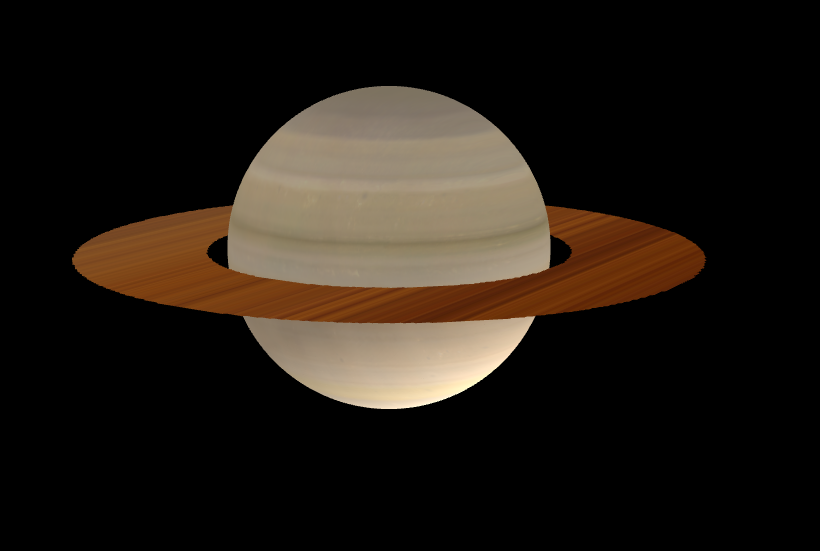
\includegraphics[width=\textwidth]{saturno.png}
\caption{Ejemplo de utilización de meshers para generar una esfera y un disco (para generar una aproximación a Saturno). Se puede notar en el disco que la aproximación no es exacta, ya que se notan ciertos problemas de aliasing.}
\label{saturno}
\end{figure}
\clearpage

\subsection{Transformación de funciones implícitas en explícitas}
\noindent En algunas ecuaciones es sencillo convertir una función del tipo $f(x,y,z)$ en un ecuación paramétrica, ya que estas ecuaciones se pueden representar como una variable en funcion del resto de forma simple. Por ejemplo, dado $f(x,y,z)  = z- x^2 - y^2$ , la ecuación paramétrica sería: 

\begin{center}
$x(u,v) = u$\\
$y(u,v) = v$\\
$z(u,v) = u^2+v^2$\\
\end{center}

Este tipo de funciones es trivial de dibujar, basta con tomar diferentes valores de $u$ y $v$ y formar polígonos con las coordenadas obtenidas de los mismos.
Pero no en todas las funciones se puede obtener una representación simple donde una variable esté en función del resto, por lo tanto no se pueden parametrizar y dibujar con el método anterior, como es el caso de  $f(x,y,z) = 2y(y^2-3x^2)(1-z^2)+(x^2+y^2)^2-(9z^2-1)(1-z^2)$. Por dicho motivo existen los siguientes algoritmos \cite{implicitas}.
%\segment
\subsection{Interpolación lineal en una recta}
\noindent  La interpolación lineal en ${\rm I\!R} ^3$ se define como: Dados $P_1=(x_1,y_1,z_1)$ y $P_2=(x_2,y_2,z_2)$, vértices de un segmento de recta y $V_1=f(x_1,y_1,z_1)$, $V_2=f(x_2,y_2,z_2)$, valores escalares en cada vértice, se requiere hallar el punto P dentro del segmento $\overline{P_1 P_2}$ dado el valor $F=f(P)$ para ello se utiliza la siguiente ecuación: 
$$P=P_1 \dfrac{\vert V-V_2\vert}{\vert V_2-V_1\vert}+P_2 \dfrac{\vert V-V_1\vert}{\vert V_2-V_1\vert}$$

Por ejemplo, dados $P_1=(0, 1, 0)$ y $P_2=(0, 0, 0)$ con los valores escalares $V_1=2$ y $V_2=8$ respectivamente, las coordenadas de P dado $V=4$ se pueden ver en la Figura \ref{interpolacionlineal}.
\begin{figure}[h!]
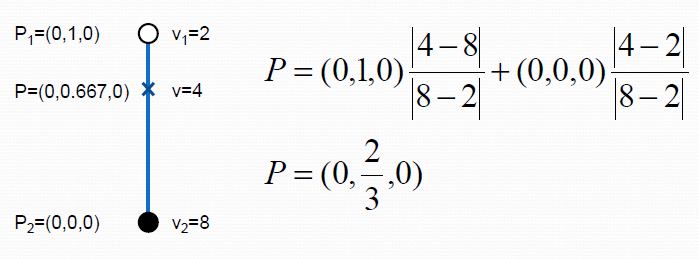
\includegraphics[width=0.7\textwidth,center]{interpolacion_ejemplo.png}
\caption{Ejemplo de interpolación lineal en el espacio}
\label{interpolacionlineal}
\end{figure}
En el contexto del proyecto debido a que se está trabajando con superficies implícitas, es decir $f(x,y,z)=0$, se requiere hallar los puntos del espacio donde la función vale 0. Para ello, cuando se requiere realizar interpolación lineal, se toman valores de $v=0$. Sin embargo, los siguientes algorítmos están pensados para funcionar con $f(x,y,z)=c$ siendo c una constante cualquiera.
\subsection{Marching Cubes}
\noindent El algoritmo de Marching Cubes\cite{marching}\cite{marchingcubes} consiste en la creación de superficies mediante la intersección de las aristas de una grilla tridimensional con el volumen de la superficie misma. Donde la superficie interseca una arista de la grilla, el algoritmo crea un vértice. Mediante la utilización de una tabla de distintos triángulos dependiendo de los diferentes patrones de intersección con la arista, el algoritmo crea una superficie.

El problema fundamental, es formar una aproximación de una superficie a través de un campo escalar dentro de una grilla rectangular 3D. Dada una celda (cubo de la grilla), definida por sus vértices y los valores escalares en cada vértice, es necesario crear caras planas que mejor representen la superficie dentro de ese cubo de la cuadrícula. La superficie puede o no pasar a través del cubo de la cuadrícula, y cortar cualquiera de los vértices. Cada posibilidad de corte con el cubo de la grilla se caracteriza por el número de vértices en que la celda tiene valores por encima o por debajo de la superficie. Si un vértice está por encima de la superficie y un vértice adyacente está por debajo de la superficie, entonces sabemos que la superficie corta el borde entre estos dos vértices. La posición en la que corta el borde será interpolada linealmente, y la relación de longitud entre los dos vértices será la misma que la relación de la superficie a los valores de los vértices del cubo de la cuadrícula.

Por convención se indexarán los vértices y aristas del cubo de la grilla de la forma que se observa en la Figura \ref{mc1}:
\begin{figure}[h!]
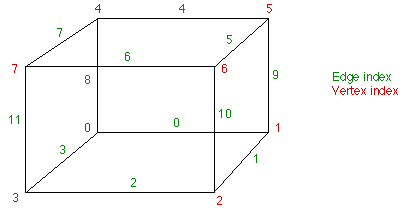
\includegraphics[width=0.75\textwidth,center]{marchingcubes1.png}
\caption{Cubo con la indexación utilizada en el algoritmo de Marching Cubes.}
\label{mc1}
\end{figure}

Si por ejemplo el valor en el vértice 3 está por debajo del valor superficie mientras los valores en todos los demás vértices están por encima del valor superficie, entonces se crea una cara triangular que corta a través de las aristas 2, 3 y 11 (ver Figura \ref{mc2}). La posición exacta de los vértices de la cara triangular depende de la relación del valor superficie a los valores en los vértices 3-2, 3-0, 3-7 respectivamente.
\begin{figure}[h!]
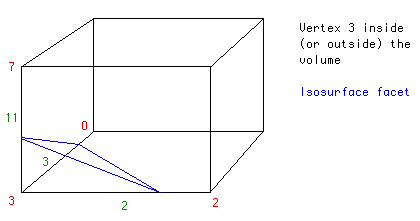
\includegraphics[width=0.75\textwidth,center]{marchingcubes2.png}
\caption{Ejemplo de creación de una cara en una celda con Marching Cubes.}
\label{mc2}
\end{figure}
Lo que hace al algoritmo ``difícil" es el gran número de combinaciones posibles (256) y la necesidad de obtener una combinación de caras consistente para cada solución, de forma que las caras generadas en las celdas adyacentes se conecten entre sí correctamente.

La primera parte del algoritmo utiliza una tabla (edgeTable) que mapea los vértices bajo la superficie a los bordes de intersección. Se forma un índice (cubeindex) de 8 bits donde cada bit corresponde a un vértice. Además se define un umbral isolevel que determina los puntos que pertenecen a la superficie y los que no.
\lstset{language=C}          % Set your language (you can change the language for each code-block optionally)

\begin{lstlisting}[frame=single][caption=blabla, label=amb]
   cubeindex = 0;
   if (grid.val[0] < isolevel) cubeindex |= 1;
   if (grid.val[1] < isolevel) cubeindex |= 2;
   if (grid.val[2] < isolevel) cubeindex |= 4;
   if (grid.val[3] < isolevel) cubeindex |= 8;
   if (grid.val[4] < isolevel) cubeindex |= 16;
   if (grid.val[5] < isolevel) cubeindex |= 32;
   if (grid.val[6] < isolevel) cubeindex |= 64;
   if (grid.val[7] < isolevel) cubeindex |= 128;
\end{lstlisting}

La búsqueda en la tabla devuelve un número de 12 bits, cada bit correspondiendo a una arista, 0 si la arista no interseca la superficie, 1 si la misma es intersecada por la superficie. Si ninguna de las aristas retorna un corte en la tabla, se devuelve un 0, esto ocurre cuando cubeindex es 0000 0000 (todos los vértices por debajo de la superficie) o 1111 1111 (todos los vértices por encima de la superficie).
Utilizando el ejemplo anterior donde sólo el vértice 3 estuvo por debajo de la superficie, cubeindex sería igual a 0000 1000 u 8, según el pseudocódigo de arriba. Con este valor de cubeindex, se pueden obtener los vértices que formarán el polígono, para ello basta con ver la celda 8 de edgeTable que tiene los valores 1000 0000 1100 ( se puede encontrar la tabla edgeTable en el Anexo I). Estos valores significan que las aristas 2, 3, y 11 son intersecados por la superficie. Los puntos de intersección se calculan ahora por interpolación lineal (Sección 3.2).

\begin{figure}[h!]
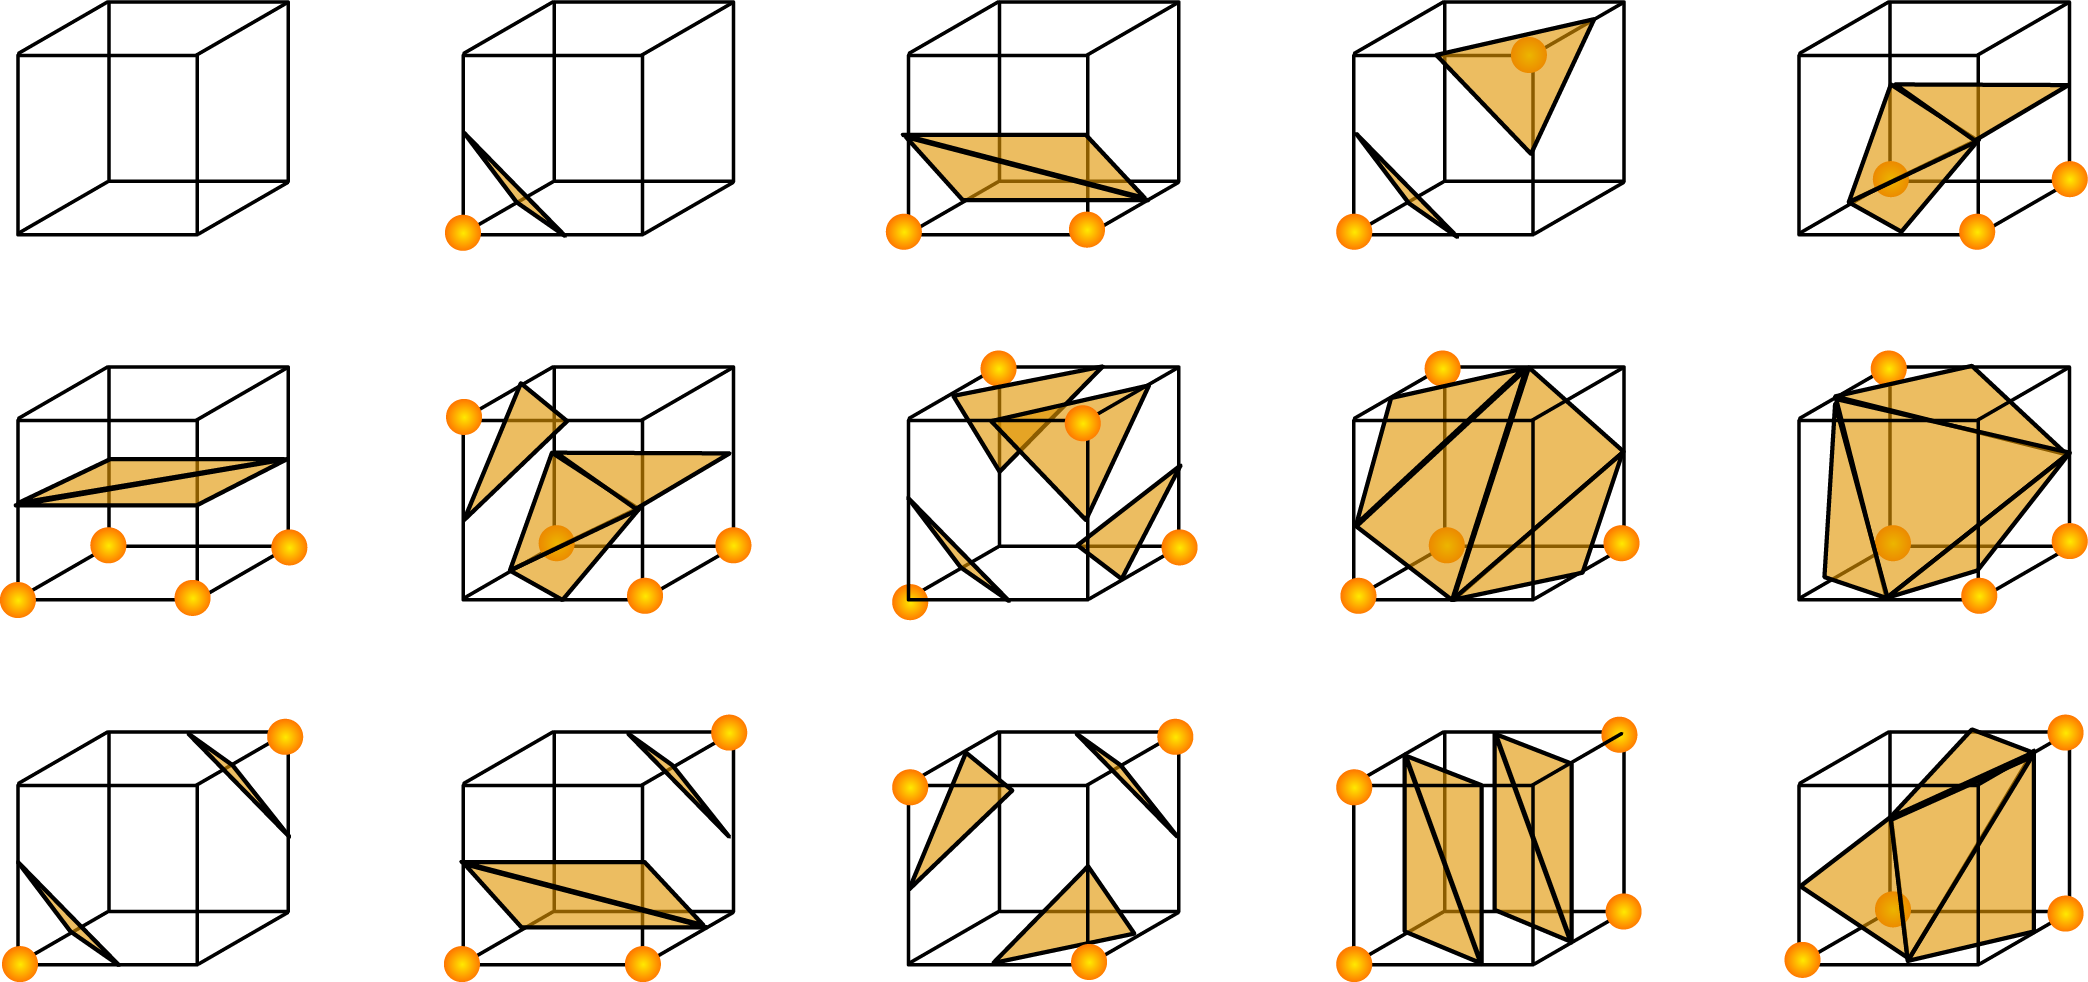
\includegraphics[width=0.8\textwidth,center]{marchingcubes3.png}
\caption{Ejemplos de formación de caras dentro de una celda.}
\label{mc3}
\end{figure}

La última parte del algoritmo implica la formación de las caras correctas en las posiciones en que la superficie interseca las aristas del cubo de la grilla, en la Figura \ref{mc3} se pueden apreciar algunos ejemplos. La tabla triTable (ver Anexo I) utiliza el cubeindex como entrada, y retorna las aristas de la grilla que  formarán parte de los vértices de las caras triangulares que sean necesarias para representar la superficie dentro del cubo de la grilla. Hay como máximo 5 caras triangulares en un cubo de la grilla.
Volviendo a nuestro ejemplo, en el paso anterior se calculan los puntos de intersección a lo largo de las aristas 2,3 y 11. El octavo elemento en la triTable es:
{3, 11, 2, -1, -1, -1, -1, -1, -1, -1, -1, -1, -1, -1, -1, -1}.

Este es un ejemplo particularmente simple, pero las combinaciones que pueden surgir no son tan evidentes para muchos de los casos de la tabla.

\subsubsection{Ambigüedades del algoritmo}
\noindent Bajo ciertos contextos  pueden ocurrir ambigüedades, es decir, situaciones donde el algoritmo puede generar dos superficies y cualquiera de las dos cumpliría con el mismo. Estas ambigüedades se resuelven en la implementación eligiendo una de las dos opciones. En la Figura \ref{ambig} se puede observar un ejemplo bidimensional.

\begin{figure}[h!]
\includegraphics[width=0.7\textwidth,center]{elquequieras.png}
\caption{Ejemplo de ambigüedad del algoritmo de Marching Cubes aplicado a una figura de 2 dimensiones. Los círculos rellenos corresponden a puntos con valor positivo, mientras que los círculos sin relleno correspnde a los de valor negativo. Se puede observar que para una misma combinación de signos pueden existir 2 figuras válidas.}
\label{ambig}
\end{figure}

\subsubsection{Resolución de la grilla}
\noindent Algo deseable a controlar cuando se poligoniza una superficie es la resolución de la cuadrícula de muestreo. Esto permite elegir el grado de la aproximación a la superficie a generarse en función de la suavidad requerida y / o la potencia de procesamiento disponible para mostrar la superficie. El ejemplo de la Figura \ref{mani} ilustra una misma superficie generada a diferentes tamaños de malla, se puede notar que en la primer figura, debido a que el tamaño de celda elegido es demasiado grande, no genera una figura correctamente.
%\clearpage
\begin{figure}[h!]
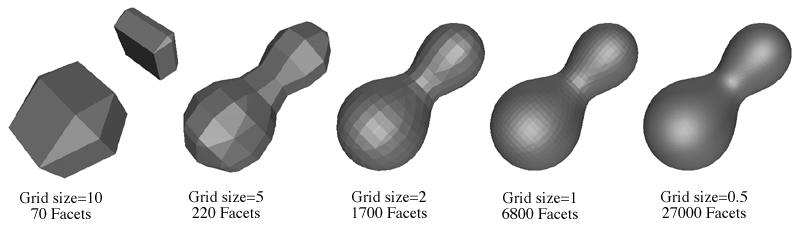
\includegraphics[width=0.8\textwidth,center]{marchingcubes4.png}
\caption{Ejemplo de la misma figura utilizando diferentes tamaños de grilla.}
\label{mani}
\end{figure}
\\\\\\

\subsection{Marching Tetrahedra}
\noindent El algoritmo Marching Tetrahedra\cite{marching}\cite{marchingt} muestrea el espacio en los vértices de una malla 3D rectangular. Cada celda de la malla se divide en 6 tetraedros como se muestra en la Figura \ref{6tet}. Hay que tener en cuenta que las aristas del tetraedro se alinean con las de las celdas de las cajas adyacentes, y existe un método de dividir la caja en 5 tetraedros que no tiene esta propiedad.

La aproximación de las caras se calcula para cada tetraedro de forma independiente. Los vértices de la cara son determinados por interpolación lineal donde la superficie corta las aristas del tetraedro.
\begin{figure}[h!]
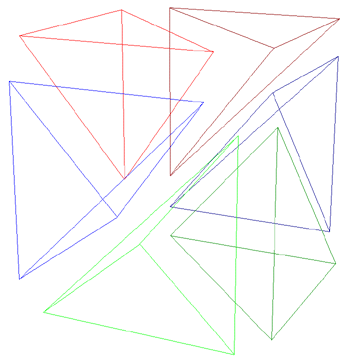
\includegraphics[width=0.6\textwidth,center]{mt1.png}
\caption{Ejemplo de división de una grilla 3D rectangular en 6 tetraedros.}
\label{6tet}
\end{figure}
%\clearpage

Hay 8 casos diferentes (ver Figura \ref{tet}). Los círculos huecos y rellenos en los vértices del tetraedro indican que los vértices están en diferentes lados de la superficie, al costado de cada ejemplo se puede ver la codificación binaria utilizada para identificar el correspondiente caso. Los casos no ilustrados se dan cuando todos los vértices están por encima o por debajo de la superficie. No se generan caras en esos 2 últimos casos.
\begin{figure}[h!]
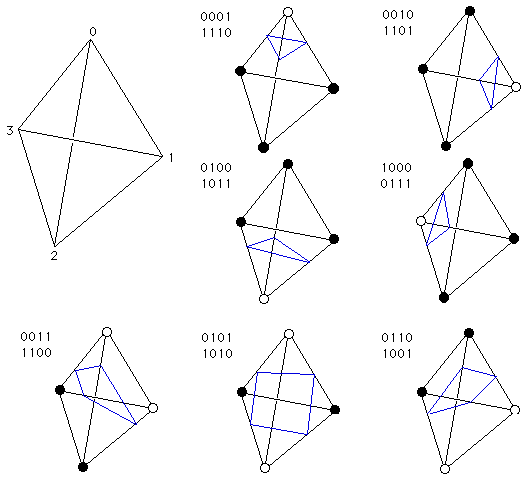
\includegraphics[width=0.7\textwidth,center]{mt2.png}
\caption{Ejemplos de generación de caras en el tetraedro.}
\label{tet}
\end{figure}\\
\textbf{Notas}
\begin{itemize}
\item Esta técnica no sufre de las ambigüedades a diferencia del algoritmo de Marching Cubes, como se puede observar en la Figura \ref{ambig}.
\item Dado que se trata de un muestreo discreto, es posible que se pierda parte de la superficie si varía dentro de una celda de la caja. Aunque éste es un problema estándar en cualquier conjunto de datos muestreados de forma discreta.
\end{itemize}

\subsection{Surface Nets}
\noindent La idea de Surface Nets es dividir el espacio en cubos, luego a cada cubo, a los que llamaremos celdas, se obtiene los signos en cada uno de sus 8 vértices, para así determinar si la celda se encuentra dentro del límite de la figura que se desea generar o no. Si los 8 vértices tienen el mismo valor ese cubo no se dibuja. En otro caso se dibuja. Ésta es la versión más simple. La imagen que se presenta en la Figura \ref{minecraft} a la izquierda utiliza ese método.
\begin{figure}[h]
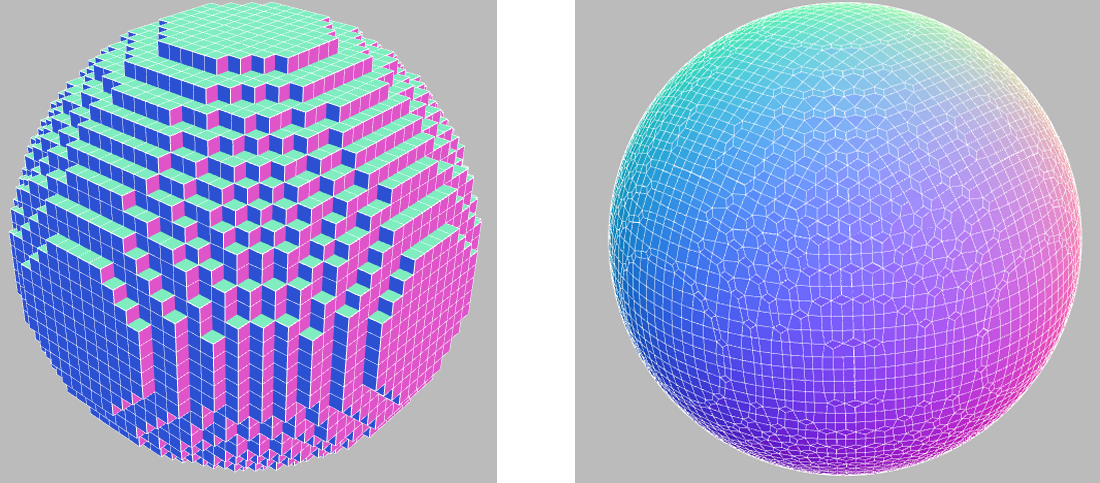
\includegraphics[width =\linewidth,center]{snc.png}
\caption{ A la izquierda se puede apreciar una aproximación de una esfera sin suavizado, mientras que a la derecha se encuentra la misma superficie con suavizado.}
\label{minecraft}
\end{figure}

El algoritmo original de Surface Nets\cite{surfacenets}, tiene una forma de “suavizar” las superficies para evitar  que la malla que genera se vea “dura”. Para lograrlo se pueden utilizar distintas técnicas de selección de los vértices, la selección de las técnicas es vital para la performance así como para la calidad de las mallas. El artículo original de Gibson[20]  propone utilizar una estrategia de minimización de la energía global y aplicarle ecuaciones de suavizado. Para hacerlo se parte de un vértice elegido al azar (en el artículo original el centro del cubo)  y se perturba (usando la técnica de descenso por el gradiente) hasta que llegue en algún momento a la superficie. Esta técnica es muy buena teóricamente, pero tiene ciertos inconvenientes de performance, ya que hay que hallar una gran cantidad de mínimos. Esto provoca (particularmente en javascript) que demore demasiado.

La idea de Naive Surface Nets (propuesto por Lysenko\cite{mykola2} y está disponible en la aplicación Isosurface) es elegir el vértice de forma más simple  en lugar de encontrar el vértice óptimo, se computan las intersecciones con las aristas de las celdas (como en Marching cubes) y luego se toma su centro de masa como el vértice en cada cubo (o celda). La malla que se obtiene de este proceso es similar a la de Marching Cubes, sólo que con un menor número de vértices y caras. Elegir el vértice de esta forma permite hacer el algoritmo mucho más rápido, aunque se pierde calidad.
\subsection{Dual Contouring}
\noindent Este algoritmo es una extensión del algoritmo de Marching Cubes y Surface Nets. Mantiene un vértice en el centro del cubo de la grilla, pero añade la generación de superficies a través de octrees, para poder dibujar más precisamente aquellas superficies “ásperas”\cite{dualcontour}. En la Figura \ref{dual} una comparación entre este algoritmo y Marching Cubes, donde se puede apreciar cómo Dual Contouring puede generar vértices dentro de las celdas para una aproximación más suave.

\begin{figure}[h!]
\includegraphics[width =\linewidth]{dualc.png}
\caption{ Comparación entre Marching Cubes (centro) y Dual Contouring (derecha), dadas las intersecciones que se muestran a la izquierda con la grilla.}
\label{dual}
\end{figure}

\subsection{Determinación de las normales de los vértices de las caras triangulares}
\noindent A menudo es necesario crear las normales para cada vértice de las caras triangulares para poder representar una superficie “suave” \cite{realtimerendering}. Ésto se debe a que para utilizar ciertas técnicas de sombreado, por ejemplo Phong, se interpola, utilizando interpolación en perspectiva, para cada píxel de cada poligono el valor de la normal de la superficie en el punto a partir de la de los vértices del mismo. Si no se cálculan las normales para cada vértice, cada cara utilizará la misma normal, lo que provocará que se visualice de forma facetada como se aprecia en la Figura \ref{normales} a la izquierda.

Una forma de realizar el cálculo de las normales para cada vértice es, después de que las caras han sido creadas, promediar las normales de todas las caras que comparten un vértice del triángulo. A continuación, en la Figura \ref{normales}, se muestra el resultado de generar una esfera utilizando el sombreado de Phong\cite{realtimerendering}, a la derecha se muestra como se visualiza suave por contar con las normales para cada vértice, mientras que a la izquierda aprecia facetada ya que se tiene una única normal cada poligono.
\begin{figure}[h]
\includegraphics[width =0.45\linewidth]{facetado.png}
\hfill
\includegraphics[width =0.45\linewidth]{noFacetado.png}
\caption{ Ejemplos de distintas configuraciones de normales de la misma figura utilizando el sombreado de Phong.}
\label{normales}
\end{figure}

Otro enfoque común es asignar a cada vértice una media ponderada de las normales de los polígonos que comparten el vértice. El peso es  inversamente proporcional al área del polígono, por lo que pequeños polígonos tienen mayor peso. La idea es que estos últimos pueden ocurrir en las regiones de alta curvatura de la superficie.

\clearpage
\section{Exploración de SURFER}
\noindent Inicialmente se investigó la posibilidad de extender las funcionalidades de SURFER para que soportase la visualización estereoscópica, por este motivo se realizaron una serie de pruebas para determinar su viabilidad. En esta sección se presentan más funcionalidades del programa junto con una explicación de las pruebas realizadas.

El programa cuenta con una interfaz amigable, a través de la cual es muy sencillo ingresar las ecuaciones. Para determinadas ecuaciones precargadas, cuenta con cierta información de modo de educar al usuario. Ésto se puede apreciar en la Figura \ref{interfazSURFER}.

\begin{figure}[h]
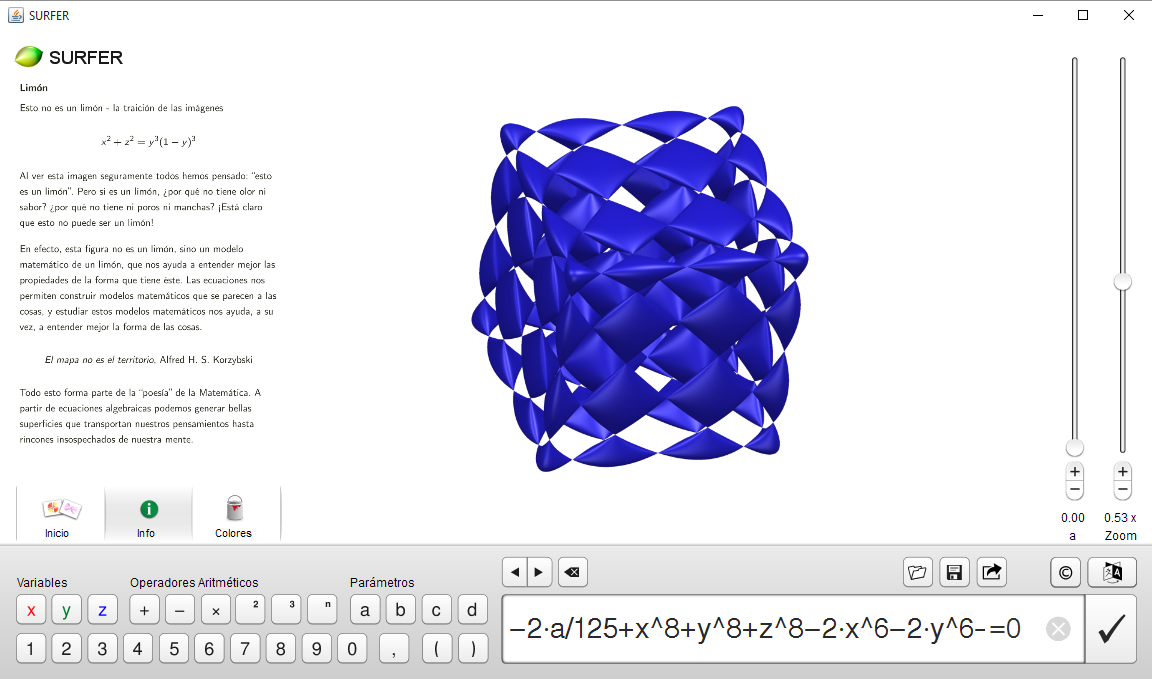
\includegraphics[width=\textwidth]{surfer_interfaz.png}
\caption{Interfaz del SURFER.}
\label{interfazSURFER}
\end{figure}

El motor utiliza el sombreado de Phong\cite{Phong} para la iluminación, por este motivo las figuras no proyectan sombras.

Al ser una aplicación que utiliza ray casting la representación de las ecuaciones que se obtiene es muy fidedigna, pero para lograr funcionar en tiempo real muestra imágenes con una baja resolución mientras se está moviendo la cámara. De esta forma se intenta mantener unos 15 fps.

Hay que destacar que en cada frame la aplicación interseca muchos rayos con la ecuación, por lo que la complejidad de la ecuación afecta la performance, es decir, la calidad la imagen  y el framerate que se obtiene depende de la ecuación. Ésto se debe a que SURFER decide la resolución de la imagen a generar de forma dinámica dependiendo del tiempo que le lleva hacerla y de si la misma se está moviendo o no, de forma de no bajar demasiado de los 15 fps.
\begin{figure}[h]
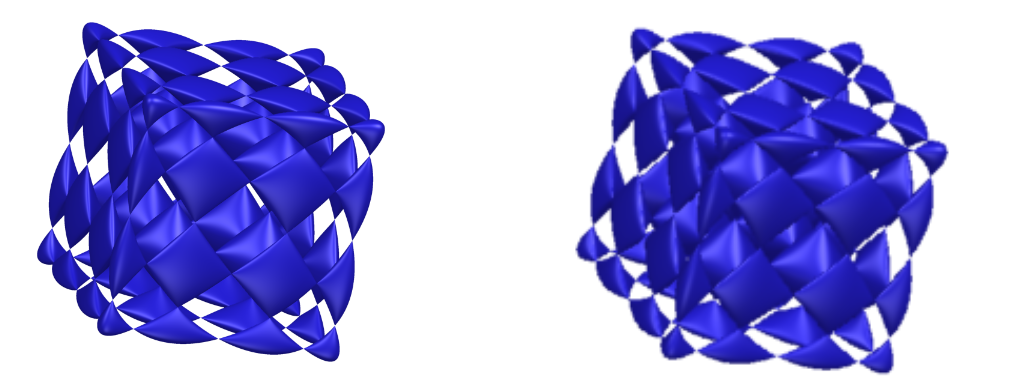
\includegraphics[width=\textwidth]{surfer_en_movimiento.png}
\caption{A la izquierda se ve la imagen una vez estabilizada, la cual posee una resolución de 796x796, mientras que a la derecha durante la rotación de la cámara la cual posee una resolución de 300x300.}
\label{malaRES1}
\end{figure}

En la Figura \ref{malaRES1} se puede apreciar cómo baja la resolución de la ecuación cuando se rota la cámara de forma  que el framerate no sufra un impacto tan grande. Hay que destacar que cuánto más cerca de la pantalla se encuentre el observador, se volverá aún más notorio el efecto de pixelación de la imagen producto de su baja resolución, perjudicando la experiencia de realidad virtual. También será muy notoria la inestabilidad en cuanto a la resolución, ya que cada vez que se rota la cámara, la resolución se reduce de forma drástica. Considerando que es muy difícil que un  usuario de Oculus Rift o similar mantenga la cabeza lo suficientemente inmóvil de manera que no baje la resolución, la mayoría del tiempo se estaría visualizando las superficies en baja resolución. El hecho de que la resolución de las imágenes es cercana a 300x300 probablemente provoque Virtual Reality Sickness (Sección 2.4).

Se intentó extender esta aplicación para darle soporte al Oculus Rift. Persiguiendo este fin se realizaron una serie de pruebas, donde se detectó que la resolución de las imágenes es demasiado pequeña cuando se intentan generar dos imágenes (una desde el punto de vista de cada ojo), aunque fuesen ecuaciones sencillas. El efecto se puede apreciar en la Figura \ref{malaRES2}. Durante el proyecto se implementó una versión modificada de SURFER. Ésta genera dos imágenes (estereoscopía) y a ambas se les aplicó la distorsión de barril. La imagen de la izquierda es cuando están quietas, la de la derecha cuando hay movimiento\footnote{Para obtener estas imágenes se modificó el nivel al que intenta mantener el framerate SURFER, el cual fue disminuido a 12fps.}.
\clearpage
\begin{figure}[h!]
\includegraphics[width=\textwidth]{se_puede_doble2.png}
\caption{A la izquierda se ve la imagen una vez estabilizada con una resolución de 796x796, mientras que a la derecha durante la rotación de la cámara con una resolución de 312x312.}
\label{malaRES2}
\end{figure}
Considerando que la aplicación genera solamente superficies algebraicas y la calidad visual obtenida cuando se generan dos imágenes de distintos puntos de vista, se decidió explorar otras opciones con la intención de poder generar un mayor número de superficies y que la experiencia de realidad virutal sea lo más placentera posible.
\clearpage
\null\newpage
\section{Alcance del proyecto}
\noindent A continuación se plantean los objetivos específicos que se consideraron a la hora de desarrollar la aplicación final. A su vez se presentan una serie de decisiones de diseño importantes que fueron tomadas a lo largo del proyecto, así como la justificación asociada.
\subsection{Objetivos}
$\bullet$ El principal objetivo del proyecto es lograr visualizar ecuaciones utilizando Oculus Rift, y donde  la experiencia del usuario sea agradable. Por ese motivo el framerate de la aplicación es importante, ya que éste debe poder mantenerse como mínimo por encima de los $60 fps$ generando dos puntos de vista distintos al mismo tiempo. Ésto persigue la disminución de la probabilidad de que los usuarios sufran VRS. 

$\bullet$ Permitir el uso de la aplicación a usuarios que no cuenten con Oculus Rift. Para ello se requiere contar con dos modalidades, una para visualizar las ecuaciones estereoscópicamente y una modalidad más simple que no lo haga.

$\bullet$ Explorar las ecuaciones de manera interactiva, pudiendo navegar por ella libremente. En particular se busca que se pueda visualizar la aplicación de dos formas, una similar a la de SURFER, donde la ecuación se encuentra en el centro y se orbita alrededor de ella; y otra similiar a los juegos en primera persona. Estas dos formas le dan al usuario la posibilidad de visualizar las superficies desde todos los ángulos posibles.

$\bullet$ Visualizar no sólo superficies algebraicas como el SURFER sino también ecuaciones implícitas en general, para darle una mayor flexibilidad al usuario.

$\bullet$ Lograr que la visualización de las ecuaciones sea lo más suave posible, es decir, que no se vean facetadas. Ésto es de suma importancia, ya que a la mayoría de los usuarios no les resulta atractivo si la figura que se obtiene se encuentra facetada.

$\bullet$ Ingresar las ecuaciones en un lenguaje simple para aumentar la usabilidad de la aplicación. Se busca que la forma de ingresar las ecuaciones sea similar al de otras herramientas matemáticas como MATLAB y Derive.

%Con la intención de hacer la aplicación lo más atractiva posible se plantearon varios objetivos en cuanto a la visualización de las superficies. Estos objetivos se encuentran la capacidad
$\bullet$ Asignar texturas a las superficies, con el fin de que los usuarios puedan tener un mayor control sobre la visualización. 

$\bullet$ Generar escenas con luces dinámicas, las cuales puedan ser modificadas por el usuario en tiempo real. Ésto permite a los usuarios tener un mayor control sobre la escena y modificarla a su gusto.

$\bullet$ Considerando el objetivo anterior, lograr que en la escena haya sombras dinámicas, ya que las sombras proveen una gran cantidad de información acerca del espacio tridimensional. La presencia de sombras es muy importante para una buena inmersión.

$\bullet$ Lograr efectos visualmente atractivos para aplicar sobre las superficies. La intención detrás de este objetivo es atraer a usuarios a la aplicación a través de los efectos visuales.

$\bullet$ Persiguiendo atraer al público más joven, así como una mayor comodidad de los usuarios, se puso como objetivo la compatibilidad con joystick.

$\bullet$ Contar con menúes en varios idiomas, de manera de hacer la aplicación accesible al mayor número de personas posible.

$\bullet$  Proveer a los usuarios una forma visual y simple de elegir qué zona se desea generar. Ésto se debe a que algunas superficies son no acotadas y a veces se debe mostrar un fragmento de la misma.

$\bullet$ Finalmente, permitir a los usuarios no visualizar una única ecuación a la vez, es decir contar con una modalidad alternativa donde se permita la visualización de varias ecuaciones al mismo tiempo. Ésto puede ser útil para que los usuarios puedan generar objetos cotidianos que sean compuestos.

\subsection{Decisiones de diseño}

$\bullet$ La principal decisión que se tomó fue no utilizar ray casting sino meshers. Esta decisión se realizó considerando la resolución de las imágenes y los framerates obtenidos utilizando ray casting. Como se presentó en la Sección 4, fue utilizada la versión modificada de SURFER desarrollada por nosotros para las pruebas. Los resultados obtenidos eran inferiores a lo recomendado para una buena experiencia estereoscópica. Por ese motivo se optó por tomar como base Isosurface (Sección 2.3.3) en lugar de SURFER. Para la toma de esta decisión también fue considerado el hecho de que de esta forma la aplicación podría generar ecuaciones implícitas, mientras que SURFER (Secciones 2.3.1 y 4 ) genera sólo ecuaciones algebraicas. Ésto permite la visualización de una cantidad mayor de superficies, aunque como se mencionó anteriormente tiene el costo de que se visualiza una aproximación poligonal, por lo que la calidad de la ecuación se ve afectada. Considerando la ganancia en performance, así como en cantidad de superficies que se pueden presentar, luego de varias pruebas, se decidió que la pérdida de calidad generada por la aproximación era aceptable. Esta decisión fue la de mayor incidencia puesto que significó abandonar lo que se había desarrollado para extender SURFER y comenzar de nuevo.

$\bullet$ Se tomó la decisión de que la aplicación fuese web. Ésto permite que un mayor número de usuarios tenga acceso a la misma, ya que no es necesario descargarla y se puede acceder desde una gran cantidad de dispositivos heterogéneos. A su vez, mejora el objetivo inicial de permitir a terceros descargar y compilar la aplicación, porque al ser ésta web, se puede directamente permitir a terceros ejecutarla desde su navegador web. 

$\bullet$ Se decidió utilizar dos patrones de diseño empleados generalmente en videojuegos, éstos son el \textit{Update Pattern} y el \textit{Game Loop Pattern}\cite{patterns}\cite{engine}. Ésto se debe a que al ser nuestro software una aplicación gráfica en tiempo real, al igual que los videojuegos, se pueden aplicar algunas de las buenas prácticas que se han desarrollado para los mismos. El \textit{Update Pattern} consiste en delegar a los diferentes elementos de la escena su actualización en la etapa previa al renderizado del frame. Ésto se efectúa en la etapa de Update o Animate, en esta etapa todos los elementos de la escena se modifican en caso de ser necesario para representar el estado actual. El \textit{Update Pattern} permite que cada objeto se responsabilice de su actualización, lo que brinda un mayor grado de independencia entre scripts. El \textit{Game Loop Pattern} consiste en contar con un loop principal, el cual es el encargado de realizar las etapas previas y renderizar los frames.  La estructura de este patrón se puede apreciar en la Figura \ref{glp}. Este patrón descompone la aplicación en tres etapas y fuerza a que cuando se ejecuta una etapa, otra no cambie el estado que influya a la misma, ya que se podrían generar inconvenientes. Por ejemplo si al mismo tiempo que se está renderizando, se actualizase la posición de un objeto, el mismo podría verse deformado, ya que algunos píxeles se podrían haber calculado antes de la actualización. Existen múltiples variantes del \textit{Game Loop Pattern}\cite{patterns}, donde se utilizan distintos criterios sobre la forma de controlar el tiempo que ha transcurrido desde el frame anterior. Se decidió emplear la versión que utiliza una variable y almacena el tiempo en milisegundos que ha transcurrido. Al decidirse que se realizaría una aplicación web, la aplicación del patrón no es la más directa, ya que a diferencia de lo que sucede en otro tipo de plataformas, la aplicación queda embebida dentro del loop del navegador. Por este motivo para utilizar este patrón se debe llamar a $requestAnimationFrame$\cite{patterns} y ejecutar las tres etapas cuando el navegador le retorna el control a la aplicación. La función $requestAnimationFrame$ permite pasarle una función al navegador para que sea llamada por él  y se ejecute. La frecuencia de las invocaciones a la función que se pasa como parámetro, depende de la configuración del navegador y de la máquina sobre la que se ejecuta. La función que recibe como parámetro $requestAnimationFrame$ es la responsable de ejecutar las tres etapas. 

\begin{figure}[h]
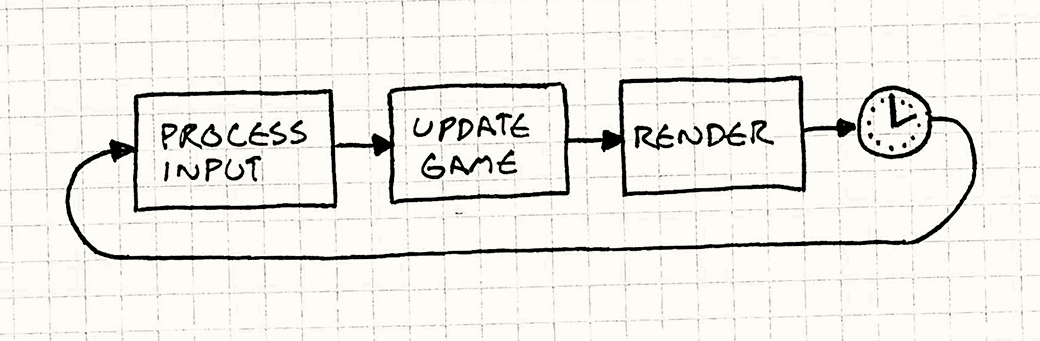
\includegraphics[width =0.8\linewidth, center]{gameloop.png}
\caption{Estructura del patrón \textit{Game Loop Pattern}\cite{patterns}.}
\label{glp}
\end{figure}

$\bullet$ Se optó por utilizar una arquitectura que siga el patrón Model-View-Controller (MVC, ver Figura \ref{mvc}), que consiste en dividir la aplicación en 3 capas interconectadas, con el objetivo de separar la representación interna de la aplicación de la capa que es presentada y visible para el usuario. Con ese fin se crean las siguientes capas: Capa de Modelo: Esta capa es la encargada, de manejar los datos, lógica y reglas de la aplicación. Capa de Vista: Esta capa es la encargada de mostrar la información al usuario. Por último, la Capa del Controlador: la misma se encarga de interpretar la entrada en comandos para la vista o el modelo.  Ésto permite modularizar los distintos componentes, para obtener asi una aplicación más mantenible, y fácil de entender, además de ser una arquitectura estándar en muchas aplicaciones web.

%\clearpage

\begin{figure}[h!]
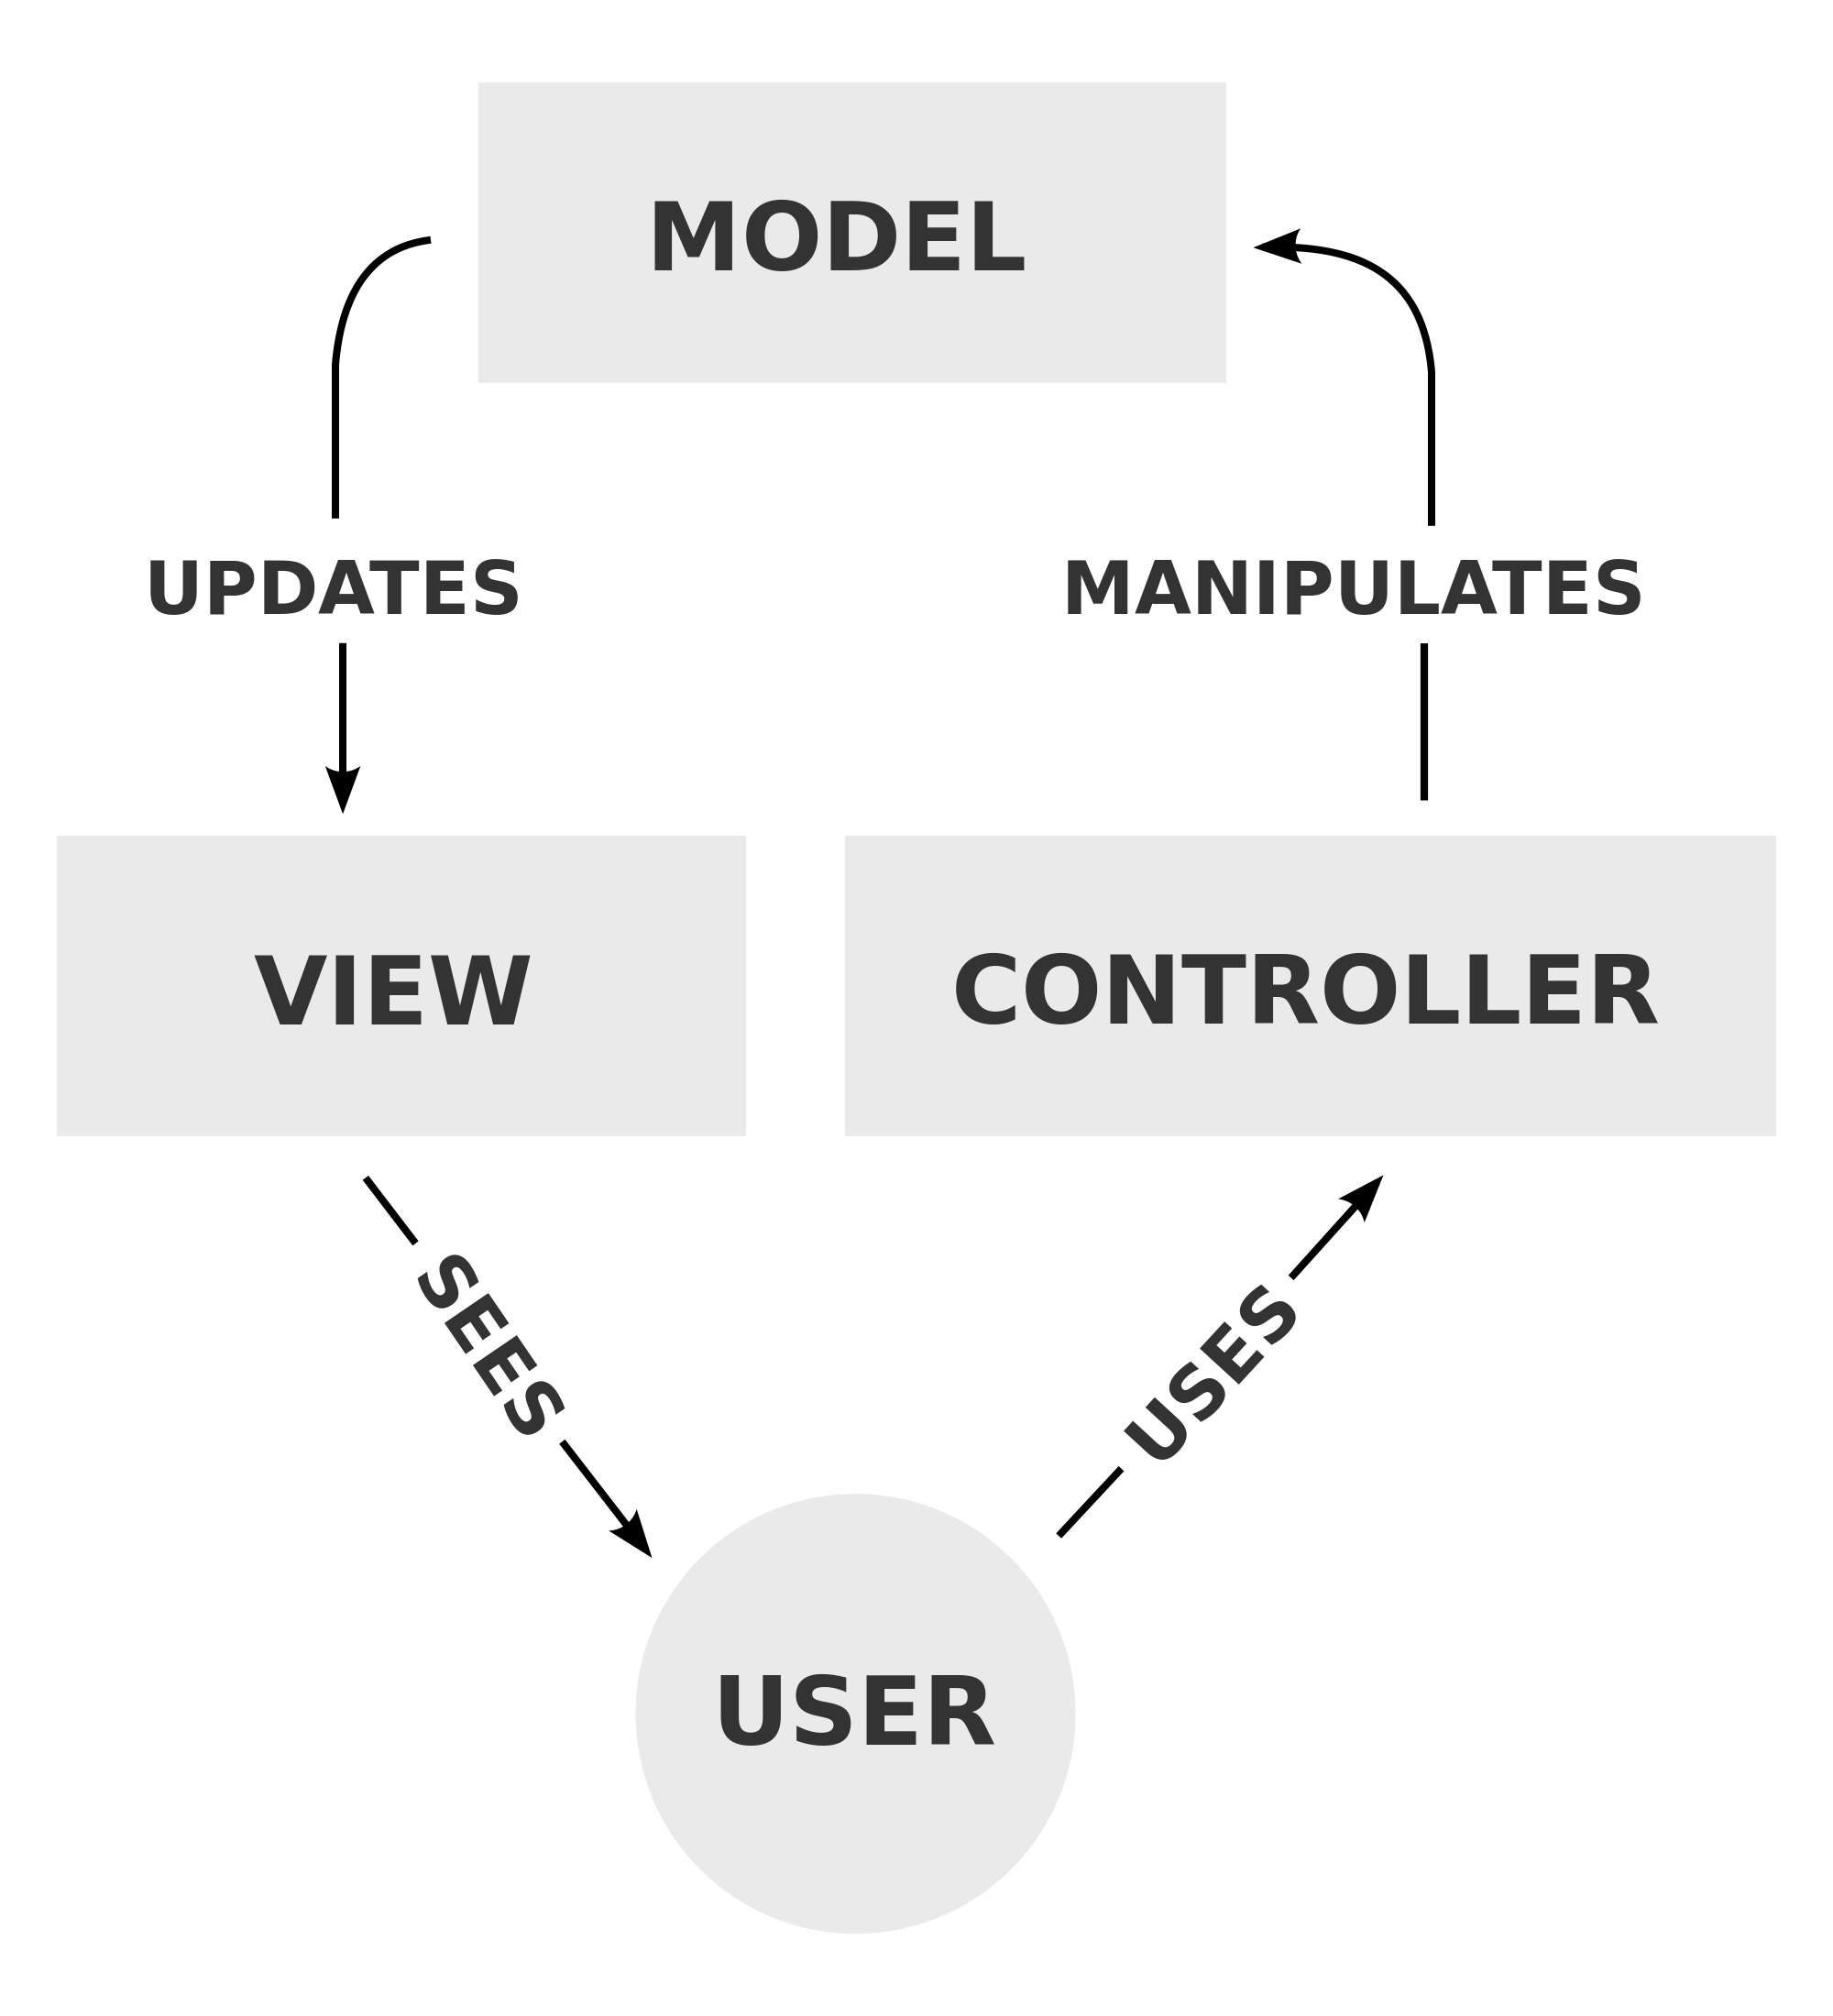
\includegraphics[width =0.5\linewidth, center]{mvc.png}
\caption{Estructura típica MVC.}
\label{mvc}
\end{figure}
$\bullet$ Buscando permitirle a los usuarios compartir y persistir las ecuaciones generadas, se decidió implementar un servicio web que brinde conectividad con una base de datos, donde los usuarios puedan almacenar las superficies deseadas junto con un nombre. A su vez la aplicación permite a usuarios ver las ecuaciones que se encuentran almacenadas en la base de datos y mostrar la que se desea. Esta función previamente chequea si hay conectividad con la base de datos, en caso de no poderse efectuar se deshabilita tanto la opción de grabar como la de cargar, pero se habilita cargar ecuaciones de una lista definida en el código de la aplicación. 

$\bullet$ Para la realización de las sombras se decidió utilizar Shadow Map\cite{shadowmap}\cite{realtimerendering}. Se decidió ésto ya que la técnica es normalmente utilizada para la realización de sombras dinámicas en los videojuegos\cite{engine}\cite{realtimerendering}. Otro factor que influyó en la decisión es el poco tiempo de renderizado extra que implica su uso. La técnica consiste en generar un mapa de profundidad (depth-map) desde la posición de la luz, y utilizarlo a la hora de sombrear cada píxel, comparando la distancia de ese punto contra la obtenida en el mapa de profundidad se decide si está iluminado por esa luz o no. Este tipo de sombras pueden sufrir problemas de aliasing y de autosombreado (self-shadowing)\cite{realtimerendering}, pero su utilización no produce un gran impacto en la performance.

$\bullet$ Para la compatibilidad del joystick se decidió utilizar polling de los valores del joystick, que es la forma comúnmente utilizada en el desarrollo de videojuegos\cite{engine}. Esto consiste en analizar en cada frame los valores de los registros del driver para verificar en qué estados se encuentran y actuar de la forma correspondiente.

$\bullet$ Se decidió agregar un módulo que se encargue de parsear las ecuaciones ingresadas para facilitar la escritura de éstas por parte del usuario. Ésto se realizó con la intención de tener una interfaz transparente, que permita ingresar las ecuaciones algebraicas de forma similar a SURFER, y usar funciones no algebreaicas como \textit{min, max, abs, funciones trigonométricas, logaritmos,etc}. Utilizando esas funciones se puede hacer Geometría Sólida Constructiva (ver Sección 7.6).

$\bullet$ Para darle al usuario un mayor grado de libertad se optó por permitir a los usuarios generar una cantidad sin límite de ecuaciones, contando con una opción que le permita elegir si quiere visualizar una única o varias. En caso de querer visualizar varias puede hacerlo con la interfaz o utilizando el teclado, donde se mapean las primeras diez ecuaciones a los números de éste. Como se mencionó anteriormente, ésto busca que los usuarios puedan generar escenas donde utilizando varias superficies puedan generar objetos cotidianos.

$\bullet$ Con la idea de permitir a los usuarios seleccionar la región que se desea generar se decidió implementar un método que presenta un cubo, el cual indica la zona que se quiere generar. Ésto permite que los usuarios generen primero un sector de un tamaño considerable con un nivel de detalle pequeño, y luego de elegir de forma visual cual es el segmento que desean ver con mayor detalle, cambiar el paso para generar con una mayor densidad la zona deseada. También permite una forma sencilla de dejar de visualizar algunos elementos que no permitan observar el detalle que se quiera por estar delante. Se puede apreciar el funcionamiento de esta herramienta en la Figura \ref{zoomCube}.

\begin{figure}[h!]
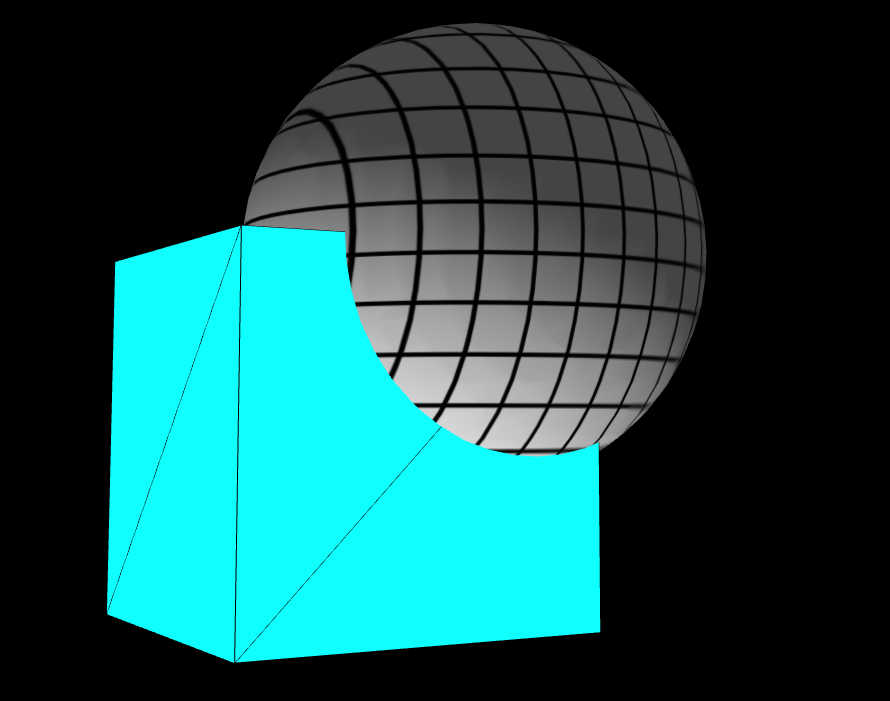
\includegraphics[width =0.45\linewidth]{cubo1.png}
\hfill
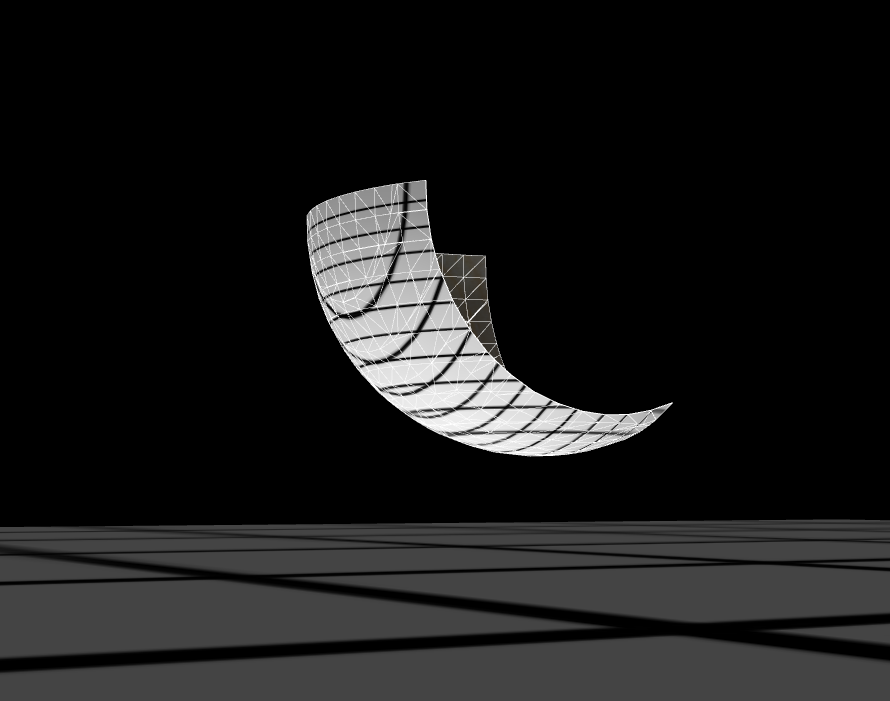
\includegraphics[width =0.45\linewidth]{cubo2.png}
\caption{ A la izquierda se puede apreciar el cubo de zoom y a la derecha el resultado de aplicarlo.}
\label{zoomCube}
\end{figure}
\clearpage
\null\newpage

\section{Solución propuesta}
$\bullet$ La aplicación es un visualizador de ecuaciones implícitas que se ejecuta en un navegador web. Ésta utiliza THREEJS junto con WebGL. La elección de usar THREEJS fue una decisión importante, ya que permite que la aplicación se pueda ejecutar en todos los navegadores modernos. Ésto busca aumentar el alcance de la aplicación, permitiendo que la misma sea accedida por cualquier persona con un navegador web moderno.

$\bullet$ La aplicación web utiliza los algoritmos presentados anteriormente basados en el trabajo de Lysenko\cite{mykola1}\cite{mykola2}, se genera una malla poligonal de las ecuaciones.  

$\bullet$ Las ecuaciones son ingresadas por el usuario utilizando una sintaxis similar a SURFER y MATLAB. Existe un módulo que se encarga de parsearlas para enviarle la información a los algoritmos de la manera que la necesitan.

$\bullet$ Para que la aplicación funcione con Oculus Rift, se utilizó MozVR lo que permite poder utilizar el dispositivo en el navegador Nightly. La aplicación también funciona con Google Cardboard en dispositivos móviles. Se decidió utilizar MozVR porque es de los pocos estándares que permiten utilizar Oculus Rift de buena forma en los navegadores web. Ésto es una restricción ya que si se desea utilizar la aplicación por sus capacidades estereocópicas en PC se deberá descargar ese navegador con el plugin de MozVR, pero para utilizar la aplicación en su forma no estereoscópica no será necesario.

$\bullet$ Para tener una arquitectura MVC bien definida se utilizó AngularJS. Se decidió utilizar este framework porque el mismo provee estructura al lenguaje Javascript, además facilita la comunicación de la vista con el controlador y el modelo, debido a que todo cambio en el controlador afecta directamente a la vista, sin necesidad de utilizar funciones de acceso a los elementos HTML. Estó permite obtener una arquitectura clara y extensible de manera sencilla.

$\bullet$ Se permite al usuario seleccionar el paso que será utilizado por el algoritmo. Es decir, el tamaño que se usa para la definición de la grilla sobre la cual se generará la malla. La grilla se genera dividiendo el intervalo ingresado de manera que cada sección de la misma posea la medida del paso. 

$\bullet$ Para obtener una mejor visualización, se propuso realizar el cálculo de las normales en cada uno  de los vértices de la superficie. Ésto, como se explicó en la Sección 3.7, permite que la visualización no sea facetada, lo que provoca que la ecuación sea visualmente más atractiva y, junto con la utilización de Phong, cumplen el objetivo de que la visualización sea ``suave". 

$\bullet$ Para navegar la superficie se decidió mostrar la geometría generada en una escena tridimensional, la cual se visualiza normalmente en un modo donde la cámara “orbita” alrededor de ecuación. Pero cuando se ingresa al modo de realidad virtual, se visualiza como si fuese en primera persona. Cuando se encuentra en dicho modo se puede usar tanto el teclado como el joystick para desplazarse alrededor de la escena de forma de poder recorrerla completamente. Ésto le da gran libertad al usuario y permite que explore la escena sin restricciones, pudiendo observar una gran cantidad de detalles que no son posibles de otra forma.

%La geometría obtenida es mostrada en una escena tridimensional, que puede ser navegada por el usuario de distintos modos, así como se le puede modificar varios parámetros, como la luz, la textura de la ecuación y hasta puede aplicarle efectos generados por shaders programados en GLSL.

$\bullet$ Para tener una variedad de efectos visuales sobre la representasión gráfica de las ecuaciones, se decidió utilizar GLSL por su gran flexibilidad, ya que es el lenguaje para la realización de shaders de openGL, además de por su interacción con THREEJS. 

$\bullet$ Con el fin de obtener la visualización de varias ecuaciones a la vez, se implementó un menú dinámico que permite la fácil adición de una superficie a la escena, además permite elegir cuáles ecuaciones ver ya sea por la interfaz en pantalla o utilizando el teclado.

$\bullet$ Con la intención de permitir a los usuarios elegir la zona de la ecuación que se quiere poligonizar, se creó un método para realizar zoom en el área deseada.  

$\bullet$ Para que los usuarios puedan compartir ecuaciones, se permite el almacenamiento en una base de datos de las mismas. Se propone implementar un web service que exponga una base de datos a la aplicación, permitiendo que los usuarios consideren interesantes, almacenando un nombre además de la ecuación y su geometría. Ésto es interesante ya que permite que se compartan ecuaciones atractivas y se trabaje en conjunto en la búsqueda de determinadas ecuaciones. 

$\bullet$ Como se mencionó anteriormente se puede utilizar Google Cardboard o Oculus Rift para experimentar la escena en realidad virtual, pudiendo ver las ecuaciones, aprovechando las técnicas de estereoscopía, con una mayor inmersión.

$\bullet$ Se propone utilizar la Gamepad API\cite{gamepadapi} para facilitar la interacción con la aplicación a través de un joystick de XBOX ONE, el cual es usado cuando se utiliza Oculus Rift. El uso del joystick de XBOX ONE (joystick oficial de Oculus Rift, el cual viene incluido en la versión de consumidor), junto con el Oculus permite atraer la atención de jóvenes hacia la aplicación. La API permite acceder de forma intuitiva a los registros del driver\cite{engine}, lo que permite realizar polling para verificar en cada frame en qué estado se encuentra el mismo.

$\bullet$ Para que las ecuaciones proyecten sombras, no sólo contra el “piso” sino que sobre sí mismas, éstas se generan utilizando la técnica de Shadow Map\cite{shadowmap}\cite{realtimerendering}.


$\bullet$ El usuario puede cambiar qué luces están activas, así como mover una de las luces de forma de poder observar mejor la ecuación. Ésto permite ver en tiempo real la variación de la sombra, así como los efectos de la luz sobre la ecuación. 
\\

Para la versión móvil se presentan ciertas carcterísticas especiales: 

$\bullet$ Durante el modo de visualización estereoscópica la figura se encuentra desplazándose circularmente, ésto permite que se pueda visualizar de todos los ángulos en el modo de realidad virtual sin tener que dejar de utilizar el Google Cardboard para poder utilizar la pantalla táctil.

$\bullet$ Por motivos de optimización se decidió quitar la generación de sombras cuando la aplicación se ejecuta desde celulares, ya que esta operación disminuye significativamente el framerate que se obtiene en los dispositivos móviles. Ésto se debe a que estos dispositivos no están pensados para este tipo de aplicación.

\clearpage
\subsection{Shaders}
\noindent Aprovechando la compatibilidad de GLSL con THREEJS y WebGL, se implementaron varios efectos interesantes, entre ellos se encuentran lava, agua y gelatina. En la Figura \ref{shader} se pueden ver algunos ejemplos.

Se implementaron vertex shaders, que son programas responsables de devolver la posición de cada vértice de la geometría en el espacio homogéneo de clipping, para realizar efectos como la vibración en la gelatina. Este tipo de shader recibe como entrada, entre otros, la posición del vértice en el espacio de coordenadas del objeto, luego debe transformarlo al espacio de proyección. Al ejecutarse una vez por cada vértice, permite transformarlos de manera de que el mismo parezca animado, por ejemplo multiplicando la posición por seno del tiempo. Ésto genera que cada vértice se mueva de forma periódica.

A su vez se utilizaron fragment shaders, que son programas encargados de retornar un color para un segmento de la superficie, para generar efectos como el de la textura del agua que actúa como si estuviese animada para generar la sensación de olas. Los fragment shaders reciben una serie de parámetros, como pueden ser texturas, posición del fragmento, normal de la superficie en el punto, coordenadas de textura, etc. Utilizando las cuentas que considere pertinente retorna un vector RGBA.

\begin{figure}[h!]
\includegraphics[width =0.32\linewidth]{shader1.png}
\hfill
\includegraphics[width =0.32\linewidth]{shader3.png}
\hfill
\includegraphics[width =0.32\linewidth]{shader2.png}
\caption{ A la izquierda se puede apreciar el efecto de lava, al centro la gelatina y a la derecha el de agua.}
\label{shader}
\end{figure}

\subsection{Texturas}
\noindent Para la utilización de texturas, se les debió asignar coordenadas de mapeo UV a las geometrías. Ésto se debe a que la forma de proyectar texturas consiste en asignarle coordenadas de textura a cada vértice. Es decir generar un mapeo que para cada vértice (representado por su posición), le corresponda una dupla (al soportar sólo imágenes bidimensionales) de números entre 0 y 1.  Estas coordenadas son interpoladas utilizando la interpolación en perspectiva para las caras\cite{realtimerendering}\cite{engine}. Luego que se tiene para cada fragmento sus coordenadas se utilizan las mismas para acceder a la imagen (tomando 0 como el primer píxel y 1 como el ancho o largo de la imagen se obtiene la posición en la misma). Para asignarles coordenadas se utilizó la proyección planar\cite{realtimerendering} (Figura \ref{texturas}).
\begin{figure}[h!]
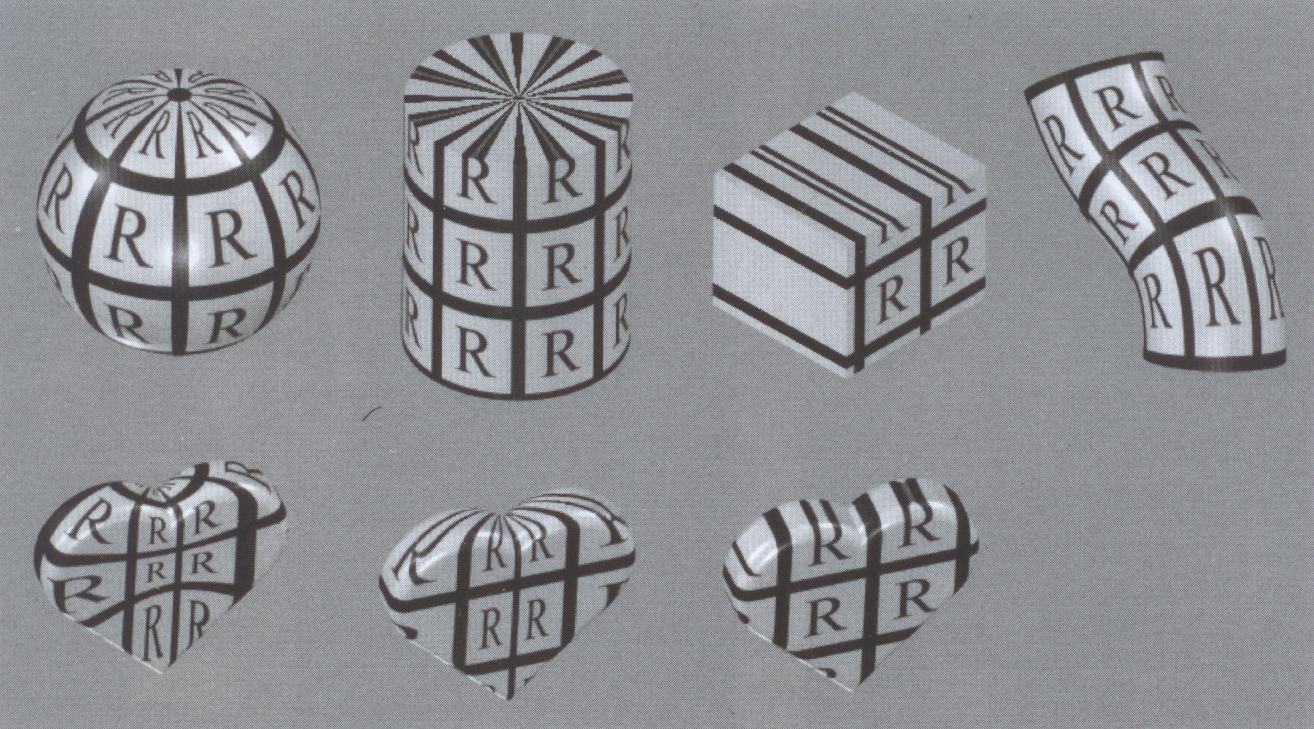
\includegraphics[width =0.5\linewidth, center]{proyecciones.png}
\caption{Tipos de proyección. De izquierda a derecha: esférica, cilíndrica, planar y natural.}
\label{texturas}
\end{figure}

Se optó por la proyección planar, debido a que es posible automatizar. La proyección natural se debe ajustar caso a caso. Se prefirió la proyección planar ante las esféricas y las cilíndricas, dado de que estas últimas sólo se ven de forma agradable sobre las figuras de características similares. En la Figura \ref{sintextura} se muestra un ejemplo, se aprecia la textura utilizada y la ecuación sin texturizar en la parte superior, mientras que en la parte inferior se observa la misma ecuación texturizada utilizando proyección planar.

\begin{figure}[h!]
\includegraphics[width =0.45\linewidth]{fondoPantalla.jpg}
\hfill
\includegraphics[width =0.45\linewidth]{sintexoc.png}
\\\\
\includegraphics[width =0.37\linewidth, center]{texturizada.png}
\caption{ Arriba a la izquierda se puede apreciar una textura, arriba a la derecha una ecuación sin texturizar y abajo la ecuación texturizada con esa textura.}
\label{sintextura}
\end{figure}

%\begin{figure}[h!]
%\includegraphics[width =0.37\linewidth, center]{texturizada.png}
%\caption{Ejemplo de superficie texturizada generada con la aplicación.}
%\label{sackboy}
%\end{figure}

\clearpage
\subsection{Arquitectura}
\noindent Como se mencionó anteriormente la aplicación cuenta con un cliente web, un backend y una base de datos. En esta sección se presentan las arquitecturas del cliente web y del backend, así como la estructura de la base de datos.
\subsubsection{Cliente web}
\noindent A continuación, en la Figura \ref{arq}, se presenta una versión simplificada del cliente web, y se provee una breve descripción de algunos de los módulos más importantes del mismo.

\begin{figure}[h!]
\includegraphics[width=\textwidth]{arq-sim2.png}
\caption{Arquitectura del cliente web.}
\label{arq}
\end{figure}
%Puso hacer descripcion general... no se que poner..

La aplicación, como se mencionó anteriormente, utiliza una arquitectura MVC. La misma  cuenta con tres services (MainService, SavingService y EquationListService que ofician de Modelo), un Controlador (Controller) y una única Vista (Interfaz). A su vez existen una serie de módulos que son utilizados por el MainService. Las partes más importantes de la aplicación se encuentran en el MainService o en Controller.

$\bullet$ El \textbf{SavingService} es el responsable de comunicarse con el backend para tanto almacenar como cargar las mallas junto con su información asociada. Este módulo es utilizado por el Controller el cual, utilizando las interfaces del MainService, le proporciona a éste la información de la malla que se recuperó de la base de datos.

$\bullet$ El \textbf{MainService} es el responsable de generar las mallas, crear la escena, hacer las actualizaciones y efectuar el render. Este módulo es el que se comunica con más módulos, ya que es el que realiza las tareas más importantes y difíciles. También es el responsable de mostrar las ecuaciones que sean pertinentes, es decir sólo aquellas que deban ser visibles en el momento dado. En este módulo se generan las coordenadas de mapeo UV, se generan los shaders, se ejecuta el main loop de la aplicación, se generan las superficies, se realizan todas las actualizaciones (posición de cámara, posición de luz, etc), se generan las texturas, se genera el cubo de zoom para recalcular la zona de la superficie que se quiera. Éste es el módulo principal de la aplicación, que utilizando el resto, efectúa la mayoría de las operaciones importantes.

$\bullet$ El\textbf{ EquationListService} posee una lista de ecuaciones que se pueden cargar. La intención de este servicio es que el usuario pueda visualizar rápidamente una serie de ecuaciones, aunque no esté conectado a la base de datos.

$\bullet$ El \textbf{Controller} es el responsable de manejar la interfaz y usar los servicios que le son provistos.

$\bullet$ Los módulos \textbf{MarchingCubes}, \textbf{Marching Tetrahedra} y \textbf{Surface Nets} implementan MarchingCubes, Marching Tetrahedra y Naive Surface Nets respectivamente, son invocados por el MainService.

$\bullet$ \textbf{AngularJS} es un framework diseñado para generar páginas web dinámicas, y el mismo extiende la sintaxis utilizada por HTML y separa la lógica de acceso a los elementos HTML, de la lógica misma de la aplicación, haciendo la aplicación ms sencilla de testear y entender. En este proyecto se utilizó para facilitar las comunicaciones entre la interfaz del menú con el servidor de backend y el MainService.

$\bullet$ \textbf{Bootstrap} es un framework enfocado en el diseño de sitios web, brindando diversos componentes comúnmente utilizado en otros sitios. Además contiene diversos templates, plantillas y objetos con diseños modernos y atractivos. 

$\bullet$ \textbf{THREEJS} es la librería presentada anteriormente, que actúa como wrapper de WebGL e implementa algunas funcionalidades de modo de permitir un uso más simple. A su vez cuenta con la ventaja de que garantiza el funcionamiento de la aplicación en los navegadores actuales, ésto permite que la misma esté disponible para la mayor cantidad de gente posible.

$\bullet$ \textbf{VREffect} es el módulo que se encarga de realizar el efecto estereoscópico, cuando la aplicación se encuentra en modo VR, se le invoca, para que genere las dos imágenes con la distorsión necesaria, para el dispositivo que se está utilizando, y con los parámetros que obtiene del navegador.

$\bullet$ \textbf{VRControls} es el responsable de que, cuando se está en modo VR, tome del dispositivo la rotación, de forma de mover la cámara de la misma forma, para poder dar la sensación de inmersión.

$\bullet$ \textbf{Gamepad} tiene el objetivo de exponer el estado del joystick de XBOX ONE utilizando la Gamepad API\cite{gamepadapi} a el MainService.

$\bullet$ \textbf{Parser} se encarga de parsear las ecuaciones ingresadas por el usuario, de manera de proveerle al MainService las ecuaciones de la forma que los algoritmos necesitan cómo entrada. Este módulo permite que el usuario no se preocupe de como requieren los algoritmos que se escriba la ecuación.
%\clearpage
\begin{figure}[h!]
\includegraphics[width=\textwidth]{arq-esp.png}
\caption{Estructura de MainService.}
\label{arqMS}
\end{figure}

En la Figura \ref{arqMS} se aprecia cómo es la estructura interna del servicio principal. Se puede observar cómo se aplicó el \textit{Game Loop Pattern} (Sección 5.2, Figura \ref{glp}), ya que el flujo del servicio se descompone en tres etapas: \textbf{Handle input}, \textbf{Update} y \textbf{Render}. También se cuenta con \textbf{Update Mesh}, que es una operación asincrónica que regenera la geometría utilizando el algoritmo seleccionado, para luego calcular sus coordenadas de mapeo UVs y las normales de los vértices.
\subsubsection{Backend y base de datos}
\noindent El backend de la aplicación fue realizado en el lenguaje Python con el framework de django y django rest framework para comunicarse con los clientes web. Éste se encarga de guardar datos de las superficies que se consideren interesantes, por ejemplo: coordenadas, nombre, cantidad de caras, etc. Todo esto se encuentra guardado en una base de datos Postgres.

Esta parte de la aplicación presenta una ventaja sobre otro tipo de aplicaciones similares, ya que permite que usuarios de distintas partes de mundol compartan ecuaciones interesantes. Además de que a medida de que más usuarios generan y almacenan ecuaciones la aplicación va creciendo en cuanto al catálogo de ecuaciones que ofrece.
\clearpage
\subsection{Interfaz}
\noindent En este punto se muestran los distintos modos con los que se puede interactuar con la aplicación. Se puede encontrar más información en el Anexo C (Manual de usuario). En la Figura \ref{pantalla} se observa la aplicación y se marcan los distintos componentes.

\begin{figure}[h]
\includegraphics[width=\textwidth,center]{pantalla-aplicacion.png}
\caption{Captura de pantalla que muestra la aplicación que muestra los distintos sectores.}
\label{pantalla}
\end{figure}

\subsubsection{Menú lateral}
\noindent La aplicación cuenta con un menú lateral, donde se puede controlar una serie de parámetros. En ese menú se ingresa la ecuación, así como se configura una serie de parámetros, como la zona que se quiere generar, el paso del algoritmo, qué algoritmo se desea utilizar, si se quiere visualizar una única ecuación o múltiples, etc. 
\subsubsection{Mensajes}
\noindent La interfaz también cuenta con una serie mensajes. Éstos son pequeños carteles que aparecen arriba a la derecha, al momento de ingresar a la página se muestra un mensaje de bienvenida en verde. 

El manejo de errores de la aplicación se hace utilizando el mismo sistema de mensajes. En el momento en que acontece un error se muestra en la misma posición que el mensaje de bienvenida, un cartel explicando el error pero con fondo rojo. Los errores pueden variar en cuanto al tipo, por ejemplo el error podría ser que el usuario ingreso una ecuación cuyos paréntesis están desbalanceados.
\subsubsection{Teclado y Mouse}
\noindent También se puede interactuar con la aplicación utilizando el teclado y el mouse, aunque el uso del teclado para afectar la escena puede ser habilitado/deshabilitado utilizando el menú lateral mencionado previamente.

El mouse se utiliza principalmente para controlar la cámara cuando no se está utilizando Oculus Rift. La aplicación cuenta con dos modos, uno en el cual se orbita alrededor de la ecuación y otro donde la cámara se comporta como si fuese en primera persona, es decir permitiendo mirar hacia los costados fijando la posición de la misma.

Por otra parte se puede utilizar el teclado para una gran cantidad de funciones. Entre ellas se encuentra desplazarse, mover las luces, cambiar el material de la ecuación, cambiar la ecuación, activar/desplazar/agrandar/achicar el cubo de zoom, etc. La mayoría de las funciones de la aplicación se pueden realizar apretando una serie de teclas.

Para más información acerca de la función de cada una de las teclas dirigirse al Anexo C, donde se encuentra el manual de usuario.

%\clearpage

\subsubsection{Joystick}
\noindent La aplicación también se puede utilizar con el joystick de XBOX ONE (Figura \ref{xbox}). El cual permite, cuando se encuentra en modo VR, desplazarse de forma más intuitiva y cómoda que si se utilizase el teclado. El mismo puede conectarse de forma inalámbrica.\\
\begin{figure}[h!]
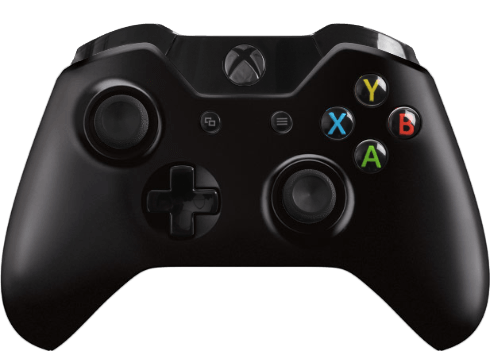
\includegraphics[width=0.5\textwidth,center]{joystickPosta.png}
\caption{Joystick de XBOX ONE.}
\label{xbox}
\end{figure}

El joystick permite una gran flexibilidad ya que puede utilizarse de forma más sencilla que un teclado cuando se está utilizando el Oculus Rift. Ésto se debe en parte, en que es más simple utilizarlo sin verlo. Aumenta significativamente el grado de usabilidad de la aplicación, ya que se vuelve más sencilla de utilizar para los usuarios, principalmente para las personas que tienen mayor experiencia con un joystick.
\clearpage
\null\newpage
\section{Análisis experimental}
\noindent En esta sección se presentan los experimentos que realizamos sobre el sistema, así como los resultados obtenidos. Las pruebas se dividen en cinco tipos, el primero es una comparación entre la performance y los resultados obtenidos utilizando cada uno de los 3 algoritmos. El segundo tipo, es cuántos fps se lograron obtener para una serie de ecuaciones, considerando la cantidad de polígonos que había en la escena. El tercero es una comparación entre SURFER y nuestra aplicación cuando se trata de puntos singulares (puntos especiales donde nuestra aplicación genera algunos artefactos). Los últimos dos tipos son una serie de operaciones interesantes que permite realizar la aplicación y una galería de imágenes.
\subsection{Hardware y Software utilizado}
\noindent Las pruebas en PC se realizaron sobre un notebook Alienware M17xR4. El cual cuenta con un procesador Intel I7-3840QM de 2.8 GHz con Turboboost hasta 3.8 GHz. La memoria RAM es de 32 GB de 1777 MHz, y cuenta con una tarjeta de video NVIDIA 680M. Se utilizó un Oculus DK1 y un Oculus DK2 como dispositivos de realidad virtual. La aplicación se testeó utilizando Firefox Nightly 48.0a1 con el plugin Mozilla WebVR plus 0.5.0. Se utilizó el runtime de Oculus 0.8.0.0. Todo se ejecutó sobre Windows 10.

En las plataformas móviles, se utilizó un Samsung  Galaxy S5 y un Samsung  Galaxy Note3, junto con un Google Cardboard. La ejecución fue sobre Google Chrome.

\subsection{Comparación entre meshers}
\subsubsection{Comparación a través de sucesiones}
\noindent La primer prueba que se realizó persiguió medir el tiempo que le lleva a cada algoritmo generar las mallas de las superficies. Para medirlo se fijó la bounding box y el paso del algoritmo, se utilizó una serie de superficies, generándolas con los tres meshers y registrando sus tiempos. Este tipo de comparación fija la información de la función que se utiliza para la generación de la geometría, pero los distintos algoritmos generan distintas cantidades de caras.

Se utilizó como intervalo $[-1,1]$ en los tres ejes, y el paso fue 0.05 (la variación en los tres ejes que utilizan los algoritmos para generar la grilla). La serie que se utilizó fue $F_n(x,y,z) = cos(\frac{n\pi x}{2}) + cos(\frac{n\pi y}{2}) +cos(\frac{n\pi z}{2}) =0$, donde $n$ varía entre 1 y 10, en las Figuras \ref{ejsuc1} y \ref{ejsuc2} se aprecian algunas de las superficies que forman parte de la serie. Se decidió utilizar esa serie ya que es similar a la utilizada por Lysenko en una de sus pruebas. Los tiempos de la Tabla \ref{suc2} son en segundos y son el promedio de 15 ejecuciones.\\\\\\\\\\

\begin{table}[h!]
  \centering
\begin{tabular}{lllllll}
\toprule 
    Valor de n & \multicolumn{2}{c}{Surface Nets} & \multicolumn{2}{c}{Marching Tetrahedra}  & \multicolumn{2}{c}{Marching Cubes}\\
    &Tiempo (s) &Caras
    &Tiempo (s) &Caras
    &Tiempo (s) &Caras \\
    \midrule
    1 & 0,016 &6 & 0,029 &119 & 0,022 &43\\
    2 & 0,080 &12168 & 0,375 &35544 & 0,091 &12680\\
    3 & 0,088 &17106 & 0,534 &51047 & 0,132 &18387\\
    4 & 0,196 &24912 & 0,618 &71520 & 0,311 &25984\\
    5 & 0,134 &30174 & 0,822 &89599 & 0,345 &32303\\
    6 & 0,178 &36312 & 1,203 &106512 & 0,349 &37968\\
    7 & 0,189 &43218 & 1,384 &127987 & 0,432 &46447\\
    8 & 0,220 &44544 & 1,434 &411264 & 0,478 &92928\\
    9 & 0,238 &56118 & 1,565 &165653 & 0,520 &60153\\
    10 & 0,345 &63480 & 1,840 &179352 & 0,671 &67240\\
    \bottomrule
\end{tabular}
  \caption{Comparación de tiempos de generación de las mallas para la serie de funciones.}
  \label{suc2}
\end{table}

\begin{figure}[h!]
\includegraphics[width =0.45\linewidth]{n3.png}
\hfill
\includegraphics[width =0.45\linewidth]{n5.png}
\caption{ A la izquierda se visualiza la función con n = 3, a la derecha con n = 5.}
\label{ejsuc1}
\end{figure}

\begin{figure}[h!]
\includegraphics[width =0.45\linewidth]{n9.png}
\hfill
\includegraphics[width =0.45\linewidth]{n10.png}
\caption{ A la izquierda se visualiza la función con n = 9, a la derecha con n = 10.}
\label{ejsuc2}
\end{figure}

Luego, considerando que Marching Tetrahedra genera alrededor de 3 veces más caras que el Naive Surface Nets y Marching Cubes (que genera en la mayoría de los casos una cantidad ``similar"), se decidió comparar el tiempo que lleva generar la superficies con cada algoritmo cuando la cantidad de caras es similar. Para lograrlo se crearon las mismas ecuaciones pero con distintos pasos. Se utilizó 0.05 como paso en Marching Cubes y Naive Surface Nets; mientras que 0.085 para Marching Tetrahedra (el número se obtuvo experimentalmente). Los resultados se pueden ver en la Tabla \ref{tablaSIC}. Como las ejecuciones anteriores para Naive Surface Nets y Marching Cubes ya utilizaban ese paso sólo se ejecutó nuevamente la parte de Marching Tetrahedra.

\begin{table}[h!]
  \centering
\begin{tabular}{lllllll}
\toprule 
    Valor de n & \multicolumn{2}{c}{Surface Nets} & \multicolumn{2}{c}{Marching Tetrahedra}  & \multicolumn{2}{c}{Marching Cubes}\\
    &Tiempo (s) &Caras
    &Tiempo (s) &Caras
    &Tiempo (s) &Caras \\
    \midrule
    1 & 0,016 &6 & 0,017 &286 & 0,022 &43\\
    2 & 0,080 &12168 & 0,156 &13032 & 0,091 &12680\\
    3 & 0,088 &17106 & 0,191 &20690 & 0,132 &18387\\
    4 & 0,196 &24912 & 0,288 &26292 & 0,311 &25984\\
    5 & 0,134 &30174 & 0,324 &36066 & 0,345 &32303\\
    6 & 0,178 &36312 & 0,389 &39556 & 0,349 &37968\\
    7 & 0,189 &43218 & 0,413 &50506 & 0,432 &46447\\
    8 & 0,220 &44544 & 0,455 &52958 & 0,478 &92928\\
    9 & 0,238 &56118 & 0,596 &64136 & 0,520 &60153\\
    10 & 0,345 &63480 & 0,794 &66634 & 0,671 &67240\\
    \bottomrule
\end{tabular}
  \caption{Comparación de tiempos de generación de las mallas para la serie de funciones para una cantidad de caras similar.}
  \label{tablaSIC}
\end{table}

\subsubsection{Comparación a través de ecuaciones puntuales}
\noindent A continuación se realizaron ciertas ecuaciones con los tres algoritmos con la intención de observar las mallas obtenidas, y analizar su similitud a la superficie real. Hay que considerar que al comparar imágenes observándolas el análisis es subjetivo. Por este motivo se presentan las imágenes, las cuales muestran además de la figura la malla para una mejor comprensión. El orden de las imágenes es análogo a la tabla. Además de las imágenes comparativas se colocó una tabla que contiene la cantidad de vértices y caras de cada figura para cada algoritmo. Las caras son todas triangulares, por lo que Surface Nets, que genera caras rectangulares se contó cada una como dos (se dividieron en dos triángulos).

Primero se realizó una esfera con el paso en 0.1 como se aprecia en la Figura \ref{esf1g}.

\begin{figure}[h!]
\includegraphics[width=\linewidth,center]{compec1.png}
\caption{Esfera generada utilizando los 3 algoritmos. A la izquierda utilizando Naive Surface Nets, al centro Marching Tetrahedra y a la derecha Marching Cubes.}
  \label{esf1g}
\end{figure}

Se puede apreciar, en el sector superior a la derecha de la esfera, cómo Marching Tetrahedra genera una superficie más suave que los otros dos. En la Figura \ref{acercamientoEsf} se muestra un acercamiento.

\begin{figure}[h!]
\includegraphics[width=\linewidth,center]{zoomesfera.png}
\caption{Acercamiento a la esfera generada utilizando los 3 algoritmos, donde se aprecia que Naive Surface Nets (izquierda) genera la geometría menos suave, mientras que Marching Tetrahedra (centro) la mejor.}
\label{acercamientoEsf}
\end{figure}

Con una segunda ecuación perteneciente a la familia de ecuaciones de Óctica de Chmutov, la cual se puede observar generada por SURFER en la Figura \ref{CHSURFER}, se obtuvo lo que se muestra en la Figura \ref{ecuacionG} con un paso de 0.05.

\begin{figure}[h!]
\includegraphics[width=0.5\linewidth,center]{ecuacion.png}
\caption{Ecuación  perteneciente a la familia de ecuaciones de Óctica de Chmutov generada con SURFER.}
\label{CHSURFER}
\end{figure}
%\clearpage%a ver

\begin{figure}[h!]
\includegraphics[width=\linewidth,center]{compec2.png}
\caption{Ecuación perteneciente a la familia de Óctica de Chmutov generada utilizando (de izquierda a derecha)  Naive Surface Nets, Marching Tetrahedra y  Marching Cubes.}
  \label{ecuacionG}
\end{figure}

Finalmente con un cilindro se obtuvo lo que se muestra en la Figura \ref{cilindro1G}  utilizando un paso de 0.1.

\begin{figure}[h!]
\includegraphics[width=\linewidth,center]{compec3.png}
\caption{Cilindro generado utilizando los 3 algoritmos.  A la izquierda utilizando Naive Surface Nets, al centro Marching Tetrahedra y a la derecha Marching Cubes.}
  \label{cilindro1G}
\end{figure}

Se puede apreciar en el cilindro arriba a la izquierda  como Marching Tetrahedra genera una superficie más suave.

En la Tabla \ref{cip} se observa cómo varía la cantidad de vértices y caras para las superficies de las imágenes anteriores. En la misma se puede apreciar como Marching Tetrahedra genera alrededor de 3 veces más caras que los otros dos algoritmos, que generan entre sí una cantidad similar.
\clearpage
\begin{table}[h!]
  \centering
  \begin{tabular}{cccc}
    \toprule
    & Surface Nets & Marching Tetrahedra & Marching Cubes\\
    \midrule
    Esfera&&&\\
    Cantidad de vértices & 392 & 6840 & 1560\\
    Cantidad de caras & 780 & 2280 & 776\\
\hline
     Óctica de Chmutov&&&\\
     Cantidad de vértices & 23432 & 430128 & 94368\\
    Cantidad de caras & 47184 & 143376 & 47504\\
\hline
     Cilindro&&&\\
    Cantidad de vértices & 3578 & 75960 & 14304\\
    Cantidad de caras & 7152 & 25320 & 7148\\
\bottomrule
  \end{tabular}
  \caption{Comparación de cantidad de caras y vértices a igual paso utilizando los 3 algoritmos.}
  \label{cip}
\end{table}

%\clearpage
De forma análoga a la sección anterior, se ejecutaron las mismas pruebas pero, en lugar de fijar el paso, se fijó la cantidad de caras, es decir, manteniendo la cantidad de caras generadas por cada algoritmo relativamente iguales.

Primero se generó la esfera, utilizando 0.05 como paso para Marching Cubes y Naive Surface Nets; mientras que 0.085 para Marching Tetrahedra. El resultado se aprecia en la Figura \ref{esfera22G}.

\begin{figure}[h!]
\includegraphics[width=\linewidth,center]{esfera2.png}
\caption{Esfera generada utilizando los 3 algoritmos.  A la izquierda utilizando Naive Surface Nets, al centro Marching Tetrahedra y a la derecha Marching Cubes.}
\label{esfera22G}
\end{figure}

Es notorio que la aproximación de Marching Tetrahedra es la más deficiente, pudiendo observarse en el sector inferior izquierdo. Ésto se puede apreciar de manera más clara en la Figura \ref{sinNombre}.

\begin{figure}[h!]
\includegraphics[width=\linewidth,center]{zoomesferamp.png}
\caption{Acercamiento a la esfera utilizando los 3 algoritmos.  A la izquierda utilizando Naive Surface Nets, al centro Marching Tetrahedra y a la derecha Marching Cubes.}
\label{sinNombre}
\end{figure}

Más adelante se generó la ecuación perteneciente a la familia de Óctica de Chmutov, utilizando 0.05 como paso para Marching Cubes y Naive Surface Nets; mientras que 0.085 para Marching Tetrahedra. Ésto se aprecia en la Figura \ref{ecuacion22G}.

\begin{figure}[h!]
\includegraphics[width=\linewidth,center]{ecuacion2.png}
\caption{Ecuación generada utilizando los 3 algoritmos.  A la izquierda utilizando Naive Surface Nets, al centro Marching Tetrahedra y a la derecha Marching Cubes.}
\label{ecuacion22G}
\end{figure}

En el sector inferior se aprecia nuevamente una peor aproximación en Marching Tetrahedra, en la Figura \ref{ecuacion22GZ} se muestra un acercamiento.

\begin{figure}[h!]
\includegraphics[width=\linewidth,center]{zoomecuacion.png}
\caption{Zoom a la ecuación generada utilizando los 3 algoritmos donde se aprecia como Marching Tetrahedra genera la peor maya.}
\label{ecuacion22GZ}
\end{figure}

Por último se generó el cilindro, utilizando 0.05 como paso para Marching Cubes y Naive Surface Nets; mientras que 0.085 para Marching Tetrahedra.

\begin{figure}[h!]
\includegraphics[width=\linewidth,center]{cilindro2.png}
\caption{Cilindro generado utilizando los 3 algoritmos.  A la izquierda utilizando Naive Surface Nets, al centro Marching Tetrahedra y a la derecha Marching Cubes.}
  \label{cilindro2G}
\end{figure}

En el sector inferior de la superficie se aprecia una peor aproximación en Marching Tetrahedra en la Figura \ref{cilindro2G}.

En la Tabla \ref{cii} se aprecia la cantidad de caras y vértices que componían las imágenes anteriores.

\begin{table}[h!]
  \centering
  \begin{tabular}{cccc}
    \toprule
    & Surface Nets & Marching Tetrahedra & Marching Cubes\\
    \midrule
    Esfera&&&\\
    Cantidad de vértices & 1472 & 9480  & 5880 \\
    Cantidad de caras &  2940 & 3160 & 2936 \\
\hline
     Óctica de Chmutov&&&\\
    Cantidad de vértices & 23432 & 144408  & 94368 \\
    Cantidad de caras &  47184 & 48136 & 47504 \\
\hline
     Cilindro&&&\\
    Cantidad de vértices & 14150 &  95624 & 56592 \\
    Cantidad de caras &  28296 & 30208 & 28292 \\
\bottomrule
  \end{tabular}
  \caption{Comparación de cantidad de caras y vértices a igual paso utilizando los 3 algoritmos.}
  \label{cii}
\end{table}

En estas pruebas se puede apreciar que el algoritmo Marching Tetrahedra, cuando se utiliza el mismo paso, genera aproximaciones levemente mejores, ya que son más suaves que las obtenidas con los otros dos algoritmos. Sin embargo es el más lento de los tres y genera una mayor cantidad de vértices y caras. Por otro lado, Naive Surface Nets es el más rápido de los tres, y las mallas que generan son levemente inferiores, ya que son más ``duras", a las de Marching Cubes, pero considerando su velocidad es una buena opción. Además, sus geometrías ocupan menos memoria. Marching Cubes se ubica en el medio entre los algoritmos, ya que no es el más rápido pero tampoco el más lento, y sus aproximaciones no son las mejores pero tampoco las peores.

A igual cantidad de caras, se puede notar que Marching Tetrahedra es inferior, ya que sus mallas son de peor calidad. Esto puede deberse a que al tener un paso mayor, utiliza menos información de la función ya que la misma se discretiza considerando el paso. Cuando se fija la cantidad de caras, se puede apreciar que Marching Tetrahedra es más rápido que Marching Cubes en algunos escenarios, pero no es más rápido que Naive Surface Nets.

\subsection{ Estudio de framerate}
\noindent Para realizar un análisis del framerate se colocaron distintas ecuaciones y se registró el framerate promedio luego de 1 minuto de rotar la cámara alrededor de ellas. Al ser la cantidad de polígonos  el factor de mayor incidencia en el framerate de una aplicación de este estilo, se registró solamente la cantidad de caras y no qué ecuación se utilizó.

A continuación se presenta la Tabla \ref{fps} con la cantidad de caras de la ecuación y el framerate promedio obtenido en Firefox Nightly. La resolución de la pantalla es de 1920x1080p.

\begin{table}[h!]
  \centering
  \label{tab:table1}
  \begin{tabular}{cc}
    \toprule
    Cantidad de caras & Framerate promedio (fps)\\
    \midrule
    14304 & 473\\
    79006 & 225\\
    51788 & 289\\
    40886&409\\
    776&695\\
    2797432&77\\
    \bottomrule
  \end{tabular}
  \caption{Comparación entre la cantidad de caras de la ecuación y framerate obtenido.}
\label{fps}
\end{table}

Estas pruebas se realizaron generando sólo un punto de vista, por lo que, en modo VR, el framerate sería menor. Aún así la mayoría de las pruebas poseen resultados muy superiores a los 120$fps$ (60Hz es la velocidad de refresco del DK1). Utilizando esto como refencia, la única escena que generaría problemas es la de casi tres millones de triángulos, pero para llegar a esa cantidad es necesario tener una gran cantidad de ecuaciones o poner un paso muy pequeño.

\subsection{Comparación con SURFER en puntos singulares}
\noindent Los puntos singulares son puntos donde no hay un único plano tangente. Éstos presentan inconvenientes para los algoritmos presentados, ya que los mismos no son generados de forma idónea. A continuación presentaremos una serie de imágenes para comparar los resultados que se obtienen utilizando SURFER con nuestra aplicación. 

Para hacerlo se utilizó una ecuación con 216 puntos singulares creada por Breske, Labs y van Straten \cite{216s}.
\begin{figure}[h!]
\includegraphics[width=\linewidth]{comp1.png}
\caption{Comparación de una figura con 216 puntos singulares creada por Breske, Labs y van Straten utilizando SURFER y la aplicación desarrollada.}
\label{svi1}
\end{figure}

En la Figura \ref{svi1} a la izquierda se puede apreciar la imagen generada con SURFER y a la derecha la misma imagen generada con Marching Tetrahedra en nuestra aplicación. Se puede apreciar cómo SURFER resuelve los puntos singulares de mejor forma. A su vez se puede apreciar cómo nuestra aplicación posee sombras.
%\clearpage
\begin{figure}[h!]
\includegraphics[width=\linewidth]{comp2.png}
\caption{Comparación cuando se realiza zoom hacia un punto singular de la figura anterior.}
\label{svi2}
\end{figure}
Se aprecia a la izquierda de la Figura \ref{svi2} cómo se visualiza cuando se utiliza el zoom de SURFER, y a la derecha lo que sucede si se utiliza la herramienta de zoom presentada en la Sección 5, para realizar un recálculo de la zona problemática. 

De estas pruebas se desprende que los puntos singulares pueden llegar a ser problemáticos si la malla no es lo suficientemente fina, así como que los resultados obtenidos no son tan precisos como los de SURFER. Por otra parte, si se quiere visualizar algún punto singular en particular se puede recalcular con mayor calidad obteniendo resultados de una calidad similar a la de SURFER.

\subsection{Análisis de usuarios}
\noindent Se presenta a continuación un breve resumen de lo obtenido al presentarle a los usuarios el cuestionario presentado en el Anexo G. Se realizaron pruebas con 13 individuos (estudiantes o egresados de la Facultad de Ingeniería). Primero se les permitió experimentar con la aplicación libremente por unos 10 minutos, teniendo a su disposición el manual de usuario. Luego se les solicitó que realizaran la prueba presentada en el Anexo G. Las pruebas que se realizaron en PC fueron con el Oculus Rift DK1.

Las críticas fueron positivas en general, la mayoría de los usuarios quedaron satisfechos con la aplicación. A continuación se presenta un resumen de los principales resultados obtenidos, junto con recomendaciones recibidas.

En las Tablas \ref{enc1} y \ref{enc2} se muestran las respuestas recibidas a la primer y segunda pregunta respectivamente las cuales utilizan la escalada de Likert.
\begin{table}[h!]
  \centering
  \begin{tabular}{ccc}
    \toprule
    Número de opción &  Texto de la opción &Cantidad\\
    \midrule
    1 & Muy Mala & 0 \\
    2 & Mala & 0 \\
    3 & Ni buena ni mala & 1 \\
    4 & Buena & 6\\
    5 & Muy Buena & 6\\
    \bottomrule
  \end{tabular}
  \caption{Calidad de la interfaz.}
  \label{enc1}
\end{table}
%tabla que se genera utilizando el archivo pero queda fea
\iffalse
\begin{table}[!ht]
    \label{tab:data}
    \centering
    \pgfplotstabletypeset[
      sci zerofill,
      precision=3,
      columns/Respuesta/.style={column type=r},
      columns/Cantidad/.style={dec sep align}
    ]{data1.txt}
 \caption{Calidad de la interfaz.}
  \end{table}
%grafica
  \begin{figure}[!ht]
    \centering
    \begin{tikzpicture}
      \begin{axis}
        \addplot table {data1.txt};
      \end{axis}
    \end{tikzpicture}
    \caption{Gráfica de la calidad de la interfaz según los usuarios entrevistados.}
  \label{enc1G}
  \end{figure}
\fi

Como se puede apreciar en la Tabla \ref{enc1} los usuarios no tuvieron inconvenientes con la interfaz, pudiéndola usar sin problemas.

%segunda
%\clearpage
\begin{table}[h!]
  \centering
  \begin{tabular}{ccc}
    \toprule
    Número de opción &  Texto de la opción &Cantidad\\
    \midrule
    1 & Muy Mala & 0 \\
    2 & Mala & 0 \\
    3 & Ni buena ni mala & 2 \\
    4 & Buena & 7\\
    5 & Muy Buena & 4\\
    \bottomrule
  \end{tabular}
  \caption{Forma de ingresar ecuación.}
  \label{enc2}
\end{table}
%tabla que se genera utilizando el archivo pero queda fea
\iffalse
\begin{table}[!h]
    \label{tab:data}
    \centering
    \pgfplotstabletypeset[
      sci zerofill,
      precision=3,
      columns/Respuesta/.style={column type=r},
      columns/Cantidad/.style={dec sep align}
    ]{data2.txt}
    \caption{Forma de ingresar ecuación.}
  \end{table}
%grafica
  \begin{figure}[!ht]
    \centering
    \begin{tikzpicture}
      \begin{axis}
        \addplot table {data2.txt};
      \end{axis}
    \end{tikzpicture}
    \caption{Gráfica de la calidad de la manera de ingresar la ecuación según los usuarios entrevistados.}
  \label{enc2G}
  \end{figure}
\fi
De la Tabla \ref{enc2} se desprende que a los usuarios les pareció satisfactoria la forma de ingresar las ecuaciones, siendo capaces de incorporarlas de forma bastante intuitiva . Ésto se debe a que la forma de ingresarlas es similar a la utilizada en varios programas de matemática, por lo que les fue sencillo a los usuarios reconocerla como familiar.

Los usuarios en general no tuvieron inconvenientes con las superficies generadas, aunque un usuario señaló que la esfera no era completamente esférica cuando le disminuyó el paso del algoritmo. 

La mayoría de los usuarios encontró interesante los efectos visuales aplicados a las superficies a través de los shaders. Con respecto a este tema recibimos varias recomendaciones de distintos tipos de efectos que podrían ser interesantes para agregar en alguna versión futura, entre ellos se encuentran: 
\begin{itemize}
\item que la lava se desprendiese de la ecuación
\item generar un efecto de transición donde la ecuación se hace de arena y se la lleva el viento
\item cell shading
\item que la ecuación actuase como un espejo
\end{itemize}

Ninguno de los usuarios que probó la aplicación sufrío ningún tipo de malestar o mareo. Todos los usuarios dijeron haber tenido una buena experiencia de realidad virtual, aunque un usuario mencionó que la densidad de píxeles del dispositivo no era la ideal.

En la versión móvil un usuario consultó por qué la ecuación se encontraba en un movimiento circular uniforme, si ésto era un error o no.

En general la aplicación fue muy bien recibida por los usuarios, estando la mayoría muy satisfechos con el funcionamiento de la misma.

Un usuario señaló que consideraría interesante la posibilidad de poder gráficar ecuaciones diferenciales con la aplicación. 

Otro usuario recomendó que se le pusiera sonido a la aplicación.

Una recomendación que se obtuvo por parte de uno de los usuarios, fue que para ayudar a los más inexpertos en el mundo de la matemática se podría agregar, de forma similar al ``Clip" de Word 2003, un asistente que brinde ayudas. Las mismas podrían ayudar a los usuarios a aprender aún más, a través de consejos y hasta ejercicios para que realice. Persiguiendo este fin, diseñamos a \textit{Equationcito, tu amigo imaginario}, el cual se puede apreciar en la Figura \ref{equationcito}.

\begin{figure}[h]
\includegraphics[width=0.2\textwidth,center]{equationcito.png}
\caption{Equationcito, la mascota oficial de Implicitus.}
\label{equationcito}
\end{figure}


\subsection{Composición de ecuaciones}
\noindent La aplicación desarrollada puede ser utilizada con fines pedagógicos. En esta sección se muestran algunas formas de utilizar el programa para  realizar ecuaciones de forma sencilla e intuitiva, de manera de de poder generar superficies a partir de algunas más simples.

Uno de los más útiles usos para el software desarrollado es utilizar la matemática para generar objetos conocidos del mundo real, es decir objetos cotidianos. Una forma de lograr ésto es por medio de la unión, intersección y resta de superficies. Estas tres operaciones son la base de la Geometría Sólida Constructiva, esta aplicación puede lograr cada una de las mismas de 3 formas distintas.

Estas tres operaciones permiten una increíble flexibilidad, y se pueden aprovechar para generar una gran cantidad de superficies. A continuación se muestran algunos ejemplos.\\
\begin{wrapfigure}{l}{0.4\textwidth}
\includegraphics[width=0.9\linewidth]{dodecaedro.png} 
\caption{Dodecaedro generado con la aplicación desarrollada.}
\label{dode}
\end{wrapfigure}

Se pueden ver dos ecuaciones generadas con nuestra aplicación con las operaciones expresadas anteriormente. Particularmente, en la Figura \ref{dode}, se puede apreciar un dodecaedro realizado intersecando 12 semiespacios definidos por planos, y en la Figura \ref{tornillo} un ``tirabuzón" generado a través de la resta entre un cilindro  y una ecuación similar a un resorte (se puede apreciar en la Figura \ref{grafobz}).
\\
\\
\\
\\
\\
\\
\\

\begin{figure}[h]
\includegraphics[width=0.7\linewidth,center]{tornillo.png}
\caption{Tirabuzón generado con la aplicación desarrollada.}
\label{tornillo}
\end{figure}
\subsubsection{Unión de ecuaciones}
\noindent Supongamos que contamos con dos volúmenes $f(x,y,z) \leq 0$ y $g(x,y,z) \leq 0$ (para lo que sigue se asume que el interior de las ecuaciones es negativo y el exterior positivo), si se quiere generar  $\cup(f,g)$ se puede realizar de 3 modos. En la Figura \ref{union} se puede ver el resultado de unir dos esferas.

$\bullet$ En el primer modo se le resta a la suma, la resta del valor absoluto, es decir $\cup(f,g) =  f(x,y,z) + g(x,y,z) - |f(x,y,z) - g(x,y,z)| \leq 0$. 

$\bullet$En el segundo caso se le resta a la suma la raíz cuadrada de la suma de los cuadrados de las funciones  $\cup(f,g) = f(x,y,z) + g(x,y,z) -\sqrt[2]{f^2(x,y,z) + g^2(x,y,z)}$.

$\bullet$En el tercer tipo se toma el mínimo de las dos  $\cup(f,g)=min(f(x,y,z),g(x,y,z))$
%\clearpage
\begin{figure}[h!]
\includegraphics[width=0.6\linewidth,center]{oi1.png}
\caption{Unión de dos esferas generada con la aplicación desarrollada.}
\label{union}
\end{figure}

\subsubsection{Intersección de ecuaciones}
\noindent Supongamos que se cuenta con dos volúmenes iguales a las del punto anterior y se desea intersecar, es decir calcular $\cap(f,g)$. Nuevamente se presentan tres métodos. En la Figura  \ref{inter} se aprecia el resultado de intersecar dos esferas.

$\bullet$El primero consiste en agregarle a la suma el valor absoluto de la resta  $\cap(f,g)= f(x,y,z) + g(x,y,z)+ |f(x,y,z) - g(x,y,z)|$ 

$\bullet$El segundo método consiste en sumarle a la suma la raíz cuadrada de la suma de los cuadrados de las funciones   $\cap(f,g)= f(x,y,z) + g(x,y,z)+ \sqrt[2]{f^2(x,y,z) +g^2(x,y,z)}$ 

$\bullet$Por último, el tercer método toma el máximo de las dos   $\cap(f,g)= max(f(x,y,z) , g(x,y,z))$
%\clearpage
\begin{figure}[h!]
\includegraphics[width=0.6\linewidth,center]{oi2.png}
\caption{Intersección de dos esferas generada con la aplicación desarrollada.}
\label{inter}
\end{figure}

\subsubsection{Resta de ecuaciones}
\noindent Nuevamente, partiendo de dos volúmenes, f y g, que cumplen las mismas propiedades que las anteriores, se desea obtener la diferencia entre ellas, $dif(f,g)$. En la Figura \ref{resta} se muestra la resta entre dos esferas.

$\bullet$La primer opción consiste en sumarle a la resta el valor absoluto de la suma $dif(f,g) = f(x,y,z) - g(x,y,z) + |f(x,y,z) + g(x,y,z)|$

$\bullet$La segunda consiste en sumarle a la resta la raíz cuadrada de la suma de los cuadrados $dif(f,g) = f(x,y,z) - g(x,y,z) + \sqrt[2]{f^2(x,y,z) + g^2(x,y,z)}$ 

$\bullet$Finalmente también es posible tomar el máximo entre $f$ y menos $g$, $max(f(x,y,z),-g(x,y,z))$
\begin{figure}[h!]
\includegraphics[width=0.6\linewidth,center]{oi3.png}
\caption{Resta de dos esferas generada con la aplicación desarrollada.}
\label{resta}
\end{figure}

\clearpage
\subsection{Galería}
\noindent En esta sección se muestran una serie de imágenes de superficies generadas con nuestra aplicación, junto con una breve descripción y la ecuación que debe ser ingresada a la aplicación para que se genere la malla.
\\Cubo: $((((x+y+abs(x-y))+(z)+ abs((x+y+abs(x-y))-(z)))+ (-z-2)+abs(((x+y+abs (x-y))+(z)+ abs((x+y+abs(x-y))-(z))) -(-z-2)))+(-x-2)+ abs((((x+y+ abs(x-y))+(z)+ abs((x+y+abs (x-y)) -(z)))+(-z-2) +abs(((x+y+abs(x-y))+(z)+ abs((x+y+ abs(x-y)) -(z)))- (-z-2)))- (-x-2))) + (-y-2) +abs((((( x+y + abs(x-y))+(z)+ abs((x+ y+abs(x-y))-(z)))+(-z-2)+ abs(((x+ y+ abs(x-y))+ (z)+abs((x+y+abs (x-y))-(z)))-(-z-2)))+ (-x-2) +abs((((x+y+abs(x-y))+(z)+ abs((x+y+ abs(x-y))-(z)))+(-z-2)+abs(((x+y+abs(x-y))+(z)+ abs((x+y+abs (x-y))-(z)))-(-z-2)))-(-x-2)))-(-y-2))$
\begin{figure}[h!]
\includegraphics[width=0.7\linewidth,center]{g1.png}
\caption{Cubo generado intersecando 6 semiespacios generados por planos.}
\end{figure}
\clearpage
Cubo con bordes redondeados intersecado con una esfera, al que se le restan 3 cilindros: $((x^6+y^6+z^6-1) +(x^2+y^2+z^2-1.3) +abs((x^6+y^6+z^6-1) -(x^2+y^2+z^2-1.3 ))) -(((y^2+z^2-.5) +(x^2+z^2-.5) -abs((y^2+z^2-.5)-(x^2+z^2-.5))) +(x^2+y^2-.5) -abs(((y^2+z^2-.5)+ (x^2+z^2-.5) - abs ((y^2+z^2-.5) - (x^2+z^2-.5))) -(x^2+y^2-.5))) + abs(((x^6+y^6+z^6-1) +(x^2+y^2+z^2-1.3) + abs((x^6+y^6+z^6-1) -(x^2+y^2+z^2-1.3))) +(((y^2+z^2-.5) +(x^2+z^2-.5)-abs((y^2+z^2-.5)-(x^2+z^2-.5)))+(x^2+y^2-.5)-abs(((y^2+z^2-.5)+(x^2+z^2-.5)-abs((y^2+z^2-.5)-(x^2+z^2-.5)))-(x^2+y^2-.5))))$\\ 
\begin{figure}[h!]
\includegraphics[width=0.7\linewidth,center]{g2.png}
\caption{La resta de tres cilindros a la intresección de una esfera y un cubo con los bordes redondeados.}
\end{figure}

En la Figura \ref{grafoed} se puede observar el grafo de construcción de la superficie anterior. 
\begin{figure}[h!]
\includegraphics[width=\linewidth,center]{figuraeduardo.png}
\caption{Se aprecia el grafo de construcción de la figura.}
\label{grafoed}
\end{figure}

\clearpage
Anillo: $max(max(max(y,- (x^2 + y^2 + z^2-1)), -y- 0.01), (x^2 +y^2 +z^2 - 3))$ \\
\begin{figure}[h!]
\includegraphics[width=0.7\linewidth,center]{g3.png}
\caption{Plano que se interseca con una esfera grande y se le resta una esfera de menor radio.}
\end{figure}
\clearpage
Cilindro con tapas: $((x^2/2 + y^2/2 - 1) + (z) + abs((x^2/2 + y^2/2 - 1)-(z)))+(-z-2)+abs(((x^2/2 + y^2/2 - 1) + (z) + abs((x^2/2 + y^2/2 - 1)-(z)))-(-z-2))$ \\
\begin{figure}[h!]
\includegraphics[width=0.7\linewidth,center]{g4.png}
\caption{Intersección de un cilindro con dos semiespacios.}
\end{figure}
\clearpage
Tirabuzón: $max((x^2 + y^2 - 1) ,-((x-sin(z*10) )^2 + (y -cos (z*10))^2 -0.8))$ \\
\begin{figure}[h!]
\includegraphics[width=0.7\linewidth,center]{g5.png}
\caption{Resta entre un cilindro y una ecuación similar a un resorte.}
\end{figure}

En la Figura \ref{grafobz} se puede observar el grafo de construcción de la superficie anterior. 
\begin{figure}[h!]
\includegraphics[width=\linewidth,center]{tirabuzongrafo.png}
\caption{Se aprecia el grafo de construcción de la figura.}
\label{grafobz}
\end{figure}
\clearpage
\null\newpage
\section{Conclusiones y trabajo a futuro}
\subsection{Conclusiones}
\noindent El producto final permite visualizar múltiples ecuaciones implícitas de forma atractiva, ya sea de forma estereoscópica o no. En el mismo se exploran las superficies libremente, pudiéndolas visualizar desde cualquier ángulo. A su vez, el ingreso de las ecuaciones se realiza a través de una interfaz simple, similar a la de otras herramientas matemáticas. 

La aplicación posee también luces y sombras dinámicas; texturas y efectos visuales a través de shaders, que permiten a los usuarios tener un mayor control de la escena.

También hay que destacar que la aplicación final es web, lo que implica que se encuentra disponible para una gran cantidad de dispositivos, sin ser necesario su descarga ni su compilación como se había considerado inicialmente.

A continuación se presentan tres partes, en la primera se analiza la performance de los meshers, comparándolos entre sí. 

En la segunda parte se analiza la performance de la aplicación en cuanto a fps y a la resolución de las imágenes generadas. En esta parte se comparará contra SURFER y se analizará si el framerate y la calidad de las imágenes es lo suficientemente bueno para una experiencia positiva de realidad virtual.

Finalmente se presentan las conclusiones de los experimentos con usuarios.
\subsubsection{Meshers}
\noindent Cada uno de los 3 métodos tiene sus puntos fuertes y débiles. 

$\bullet$ \textbf{Marching Cubes} es bueno ya que existen implementaciones libres y fácilmente utilizables, y también es bastante rápido, sin mencionar que también es la más ampliamente conocida. Además de ser relativamente rápido no tiene el problema de repetir vértices como es el caso de Naive Surface Nets, y la calidad de las mallas es superior. Los resultados no son tan agradables a la vista como los de Marching Tetrahedra, pero es considerablemente más veloz. 

$\bullet$ \textbf{Marching Tetrahedra} soluciona algunos problemas de Marching Cubes a expensas de ser mucho más lento y la creación de mallas de mayor tamaño. A su vez, estas últimas poseen una mayor suavidad, pero contienen mucho más caras y vértices, además  el algoritmo es mucho más lento.

$\bullet$ \textbf{Naive Surface Nets} posee una velocidad significativamente superior y se puede ampliar para generar mallas de alta calidad utilizando algoritmos más sofisticados de selección de vértices. También es fácil de implementar y produce mallas ligeramente más pequeñas en cuanto a su costo de almacenamiento. Su inconveniente principal es que las superficies que genera son de inferior calidad, aunque podría mejorarse si se cambia la técnica de elección de vértices. 

$\bullet$ La elección de cual de los métodos es el superior depende de cada caso. Si se quiere ahorrar en memoria y obtener el resultado con mayor rapidez, se debe usar Naive Surface Nets,  asumiendo que la aproximación se vería comprometida con respecto al uso de cualquiera de los otros dos algoritmos. Por otra parte, si se quiere maximizar la precisión de la aproximación se debe utilizar Marching Tetrahedra, que demorará más tiempo y utilizará más recursos. Finalmente, si se quiere una opción más equilibrada, se puede optar por Marching Cubes ya que no es tan preciso a la hora de aproximar como Marching Tetrahedra, pero es más rápido y usa menos recursos; además de que es más preciso que Naive Surface Nets aunque es más lento. Por estos motivos se optó por dejar a Marching Cubes como algoritmo por defecto, pero permitirle al usuario cambiarlo en caso de que éste lo considere necesario.

\subsubsection{Calidad de imagen y framerate}
\noindent Los framerates obtenidos son altos, ampliamente superiores a 60 fps (la tasa de refresco que los videojuegos apuntan a obtener). Son también ampliamente superiores a los 15 fps que tiene como objetivo mantener el SURFER. Ésto hace que la experiencia visual sea muy fluida y agradable (tanto en el modo de realidad virtual como en el normal). 

La resolución de las imágenes es alta, los framerates fueron tomados con una pantalla de resolución 1920x1080p, lo que es muy superior a las imágenes que genera SURFER (las cuales no superan 796x796). El hecho de que se pueda mantener un framerate tan alto con esa resolución permite disminuir el efecto de pixelación en Oculus Rift. 

El hecho de que se tienen framerates altos y resolución alta, como se dijo anteriormente, ayuda a disminuir la probabilidad de que los usuarios experimenten Virtual Reality Sickness. Lo cual es muy positivo ya que permite que la aplicación gane en usabilidad.

La experiencia obtenida utilizando la aplicación con DK1 y con DK2 ha sido muy positiva, ya que ninguno de los usuarios sufrió ningún tipo de inconveniente, ni sensación de mareo. 

Las pruebas con Google Cardboard también fueron favorables. Ninguno de los usuarios sufrió ningún tipo de inconveniente.

A su vez hay que destacar que, aunque se presenten dichas ventajas, el uso de ray casting hubiese permitido visualizar de forma más precisa algunas ecuaciones, particularmente aquellas con múltiples puntos singulares, y evitar algunos artefactos en dichos puntos. Aún así la aproximación es buena, pero la que genera SURFER es superior. Sin embargo, si se utiliza la funcionalidad de cortar y se acerca a las zonas problemáticas, el resultado obtienido es muy bueno, ya que se disminuye la aparición de la deformación.

\subsubsection{Experiencia de los usuarios}
\noindent Las pruebas realizadas con usuarios fueron muy favorables, ya que la aplicación no sufrió críticas considerables. La mayoría de los usuarios lograron utilizar la aplicación casi sin inconvenientes, y se mostraron confomes con su interfaz y la metodología para ingresar las ecuaciones.

A su vez, los usuarios quedaron satisfechos con la calidad visual de las superficies. Recibimos comentarios favorables en cuanto a los shaders, texturas e iluminación dinámica. Los usuarios expresaron un particular interés por los shaders, recomendando una gran cantidad de efectos que podrían ser agregados en futuras iteraciones. 

Los usuarios quedaron ampliamente satisfechos con la gran libertad que se les brinda a la hora de navegar la superficie, ya que con gran facilidad pueden explorarla, logrando observarla desde cualquier ángulo.

Como se mencionó anteriormente, ninguno de los usuarios sintió ningún tipo de mareo o disconformidad mientras utilizaba la aplicación. Ésto es muy importante, ya que uno de los objetivos del proyecto era poder proveer a los usuarios con una experiencia de realidad virtual de buena calidad, la cual no fuese probable que produciese VRS. 

\subsection{Trabajo a futuro}
%Para mejorar aún más la aplicación se podrían implementar una serie de cambios y agregados. 
\noindent A continuación se listan una serie de mejoras y modificaciones que se podrían implementar sobre la aplicación.

$\bullet$ Explorar la posibilidad de agregar a la lista de algoritmos de generación de malla, el algoritmo de Dual Contouring\cite{dualcontour}, el cual mejoraría los resultados en cuanto a la calidad de la geometría, aunque aumentaría el tiempo de cálculo. 

$\bullet$ En cuanto a la mejora de los algoritmos, analizar la implementación de diferentes versiones de Surface Nets, donde se cambian las técnicas de selección de los vértices, para obtener mejores resultados.

$\bullet$ Agregar otros shaders de GLSL. Ésto permitiría incorporar nuevos efectos visuales, volviéndolo más atractivo. Se podría, por ejemplo, permitir al usuario agregar sus propios shaders, de forma de otorgarle  mayor control de cómo se visualiza la ecuación. También se podría alterar algunos de los shaders existentes de manera que los clicks en pantalla afecten su comportamiento, por ejemplo que los clicks generen ondas en el agua, o que el movimiento de la ecuación afecte la vibración de la gelatina.

$\bullet$ Mejorar la interfaz en caso que se ingrese desde un teléfono, para hacerla más amigable para los dispositivos móviles. También se podrían desarrollar aplicaciones para celular (aprovechando la existencia de herramientas para utilizar HTML, CSS y Javascript para hacer aplicaciones para estos dispositivos) tanto para Android como para iOS. 

$\bullet$ Traducir el código a C++ con OpenGL, para implementar una versión de escritorio. De esta forma se mejoraría la performance porque se obtendría código compilado, además de disminuir el overhead. Por otro lado se tendría un mayor control del framerate ya que no se dependería del loop de refresco del navegador.

$\bullet$ Utilizar técnicas de simplificación\cite{simplificacion}\cite{realtimerendering} con el fin de simplificar la geometría con la menor pérdida de calidad posible. Ésto permitiría disminuir considerablemente la cantidad de polígonos en varias ecuaciones, por ejemplo, si se simplificase la ecuación del plano $x-3=0$, en lugar de tener una gran cantidad de triángulos dependiendo del paso seleccionado por el usuario, simplemente se tendrían 2 triángulos.

\clearpage
\null\newpage
\section{Glosario}
\noindent \textbf{\textit{AngularJS}} es un framework de JavaScript de código abierto, mantenido por Google, que se utiliza para crear y mantener aplicaciones web de una sola página. Su objetivo es crear aplicaciones basadas en el patrón Modelo Vista Controlador (MVC) para navegadores, su objetivo es hacer que el desarrollo y las pruebas unitarias sean más fáciles.\\
\textbf{\textit{Base de datos}} son bancos de información que contienen datos relativos a diversas temáticas y categorizados de distinta manera, pero que comparten entre sí algún tipo de vínculo o relación que busca ordenarlos y clasificarlos en conjunto.\\
\textbf{\textit{Bootstrap}} es un framework o conjunto de herramientas de código abierto para diseño de sitios y aplicaciones web. Contiene plantillas de diseño con tipografía, formularios, botones, cuadros, menús de navegación y otros elementos de diseño basado en HTML y CSS, así como, extensiones de JavaScript opcionales adicionales.\\
\textbf{\textit{CSS}} en inglés la sigla significa Cascading Style Sheets, es un lenguaje usado para definir y crear la presentación de un documento estructurado escrito en HTML o XML (y por extensión en XHTML). El World Wide Web Consortium (W3C) es el encargado de formular la especificación de las hojas de estilo que servirán de estándar para los agentes de usuario o navegadores.\\
\textbf{\textit{DJANGO}} es un framework de desarrollo web de código abierto, escrito en Python, que respeta el patrón de diseño conocido como Modelo–vista–controlador. Fue desarrollado originalmente para gestionar varias páginas orientadas a noticias de la World Company de Lawrence, Kansas, y fue liberado al público bajo una licencia BSD en julio de 2005.\\
\textbf{\textit{FPS}} del inglés frames per second, es la cantidad de imágenes que se muestra en un segundo.\\
\textbf{\textit{Git}}  es un software de control de versiones, desarrollado pensando en la eficiencia y la confiabilidad del mantenimiento de versiones de aplicaciones cuando éstas tienen un gran número de archivos de código fuente. Git se ha convertido en un sistema de control de versiones con funcionalidad plena. Hay algunos proyectos de mucha relevancia que ya usan Git.\\
\textbf{\textit{Github}} es una plataforma de desarrollo colaborativo para alojar proyectos utilizando el sistema de control de versiones Git. Utiliza el framework Ruby on Rails por GitHub, Inc. (anteriormente conocida como Logical Awesome). Desde enero de 2010, GitHub opera bajo el nombre de GitHub, Inc. El código se almacena de forma pública, aunque también se puede hacer de forma privada.\\
\textbf{\textit{Google Cardboard}} es una plataforma de realidad virtual (VR) desarrollada por Google sobre la base de cartón plegable, de allí su nombre, que funciona a partir de montar un teléfono móvil inteligente con android.\\
\textbf{\textit{GPU}} del inglés Graphics Processing Unit (Unidad de Procesamiento de Gráfico). Es un chip especializado en procesar imágenes, en especial gráficos 3D. Su propósito es acelerar los cálculos necesarios para dicho procesamiento, se caracteriza por una gran capacidad de procesamiento en paralelo de operaciones numéricas.\\
\textbf{\textit{GLSL}}  es el acrónimo de OpenGL Shading Language (Lenguaje de Sombreado de OpenGL), también conocido como GLslang, una tecnología parte del API estándar OpenGL, que permite especificar segmentos de programas gráficos que serán ejecutados sobre el GPU. Su contrapartida en DirectX es el HLSL. GLSL es un lenguaje de sombreado de alto nivel basado en el lenguaje de programación C.\\
\textbf{\textit{HTML}}  sigla en inglés de HyperText Markup Language (lenguaje de marcas de hipertexto), hace referencia al lenguaje de marcado para la elaboración de páginas web. Es un estándar que sirve de referencia del software que conecta con la elaboración de páginas web en sus diferentes versiones, define una estructura básica y un código (denominado código HTML) para la definición de contenido de una página web, como texto, imágenes, videos, juegos, entre otros. Es un estándar a cargo del World Wide Web Consortium (W3C).\\
\textbf{\textit{JavaScript}} es un lenguaje de programación interpretado, dialecto del estándar ECMAScript. Se define como orientado a objetos, basado en prototipos, imperativo, débilmente tipado y dinámico.\\
\textbf{\textit{Joystick}} es un periférico de entrada de que posee generalmente una o más palancas y varios botones, generalmente se utilizan en los videojuegos.\\
\textbf{\textit{JSON}} acrónimo de JavaScript Object Notation, es un formato de texto ligero para el intercambio de datos. JSON es un subconjunto de la notación literal de objetos de JavaScript aunque hoy, debido a su amplia adopción como alternativa a XML, se considera un formato de lenguaje independiente.\\
\textbf{\textit{Motion sickness}} significa cinetosis en inglés, es la sensación de mareo producida por el movimiento.\\
\textbf{\textit{MozVr}} es el proyecto de Mozilla para agregar la posibilidad de usar realidad virtual en páginas web (WebVR).\\
\textbf{\textit{NodeJS}} es un entorno en tiempo de ejecución multiplataforma, de código abierto, para la capa del servidor (pero no limitándose a ella) basado en el lenguaje de programación ECMAScript, asíncrono, con I/O de datos en una arquitectura orientada a eventos y basado en el motor V8 de Google. Fue creado con el enfoque de ser útil en la creación de programas de red altamente escalables, como por ejemplo, servidores web.\\
\textbf{\textit{Nightly}} es una versión modificada de Mozilla Firefox, la cual cuenta con modificaciones experimentales.\\
\textbf{\textit{Oculus Rift}} es un dispositivo que utiliza técnicas de estereoscopía para poder visualizar en 3D imágenes generadas en las computadoras.\\ 
\textbf{\textit{OpenGL}} es un framework de desarrollo para aplicaciones interactivas con gráficos 2D y 3D. Es soportado por varios sistemas operativos y modelos de tarjetas gráficas.\\
\textbf{\textit{PIP}} es un sistema de gestión de paquetes utilizado para instalar y administrar paquetes de software escritos en Python.\\
\textbf{\textit{PostgreSQL}} es un Sistema de gestión de bases de datos relacional orientado a objetos y libre, publicado bajo la licencia PostgreSQL, similar a la BSD o la MIT.\\
\textbf{\textit{Python}} es un lenguaje de programación interpretado cuya filosofía hace hincapié en una sintaxis que favorezca un código legible.\\
\textbf{\textit{REST}} transferencia de Estado Representacional (Representational State Transfer) o REST es un estilo de arquitectura software para sistemas hipermedia distribuidos como la World Wide Web. El término se originó en el año 2000, en una tesis doctoral sobre la web escrita por Roy Fielding, uno de los principales autores de la especificación del protocolo HTTP y ha pasado a ser ampliamente utilizado por la comunidad de desarrollo.\\
\textbf{\textit{Renderizar}} es el proceso utilizado para generar una imagen mediante una serie de cálculos partiendo de modelos en 3D\\
\textbf{\textit{Shader}} la tecnología shaders o sombreadores es cualquier unidad escrita en un lenguaje de sombreado que se puede compilar independientemente. Es una tecnología reciente y que ha experimentado una gran evolución destinada a proporcionar al programador una interacción con la unidad de procesamiento gráfico (GPU) hasta ahora imposible. Los shaders son utilizados para realizar transformaciones y crear efectos especiales, como por ejemplo iluminación, fuego o niebla. Para su programación los shaders utilizan lenguajes específicos de alto nivel que permitan la independencia del hardware.\\
\textbf{\textit{SQL}} es en inglés Structured Query Language (lenguaje estructurado de consulta), es un lenguaje utilizado para realizar consultas a la base de datos.\\
\textbf{\textit{THREEJS}} es una librería liviana escrita en JavaScript que permite trabajar con WebGL de forma más sencilla. En este trabajo se utilizó la versión 73.\\
\textbf{\textit{WebGL}} es la versión web de OpenGL, permite la realización de gráficos en 3D en páginas web. Es compatible con la mayoría de los navegadores modernos.\\
\textbf{\textit{XBOX ONE}} consola de videojuegos desarrollada por Microsoft, pertenece a la octava generación de consolas
\clearpage
\null\newpage
\section{Referencias}

\begin{thebibliography}{9}

\bibitem{dxplormath} 
3dxplormath organization. homepage. 
Visitado 2016-05-21 
\\\url{http://3d-xplormath.org/}

\bibitem{realtimerendering} 
Akenine-Moller, T., Haines, E., Hoffman, N. (2008). \textit{Real-Time Rendering Third Edition}, A. K. Peters, Ltd.

\bibitem{nuestrocodigo} 
Báez, G., Coore, P., (2016), \textit{Implicitus}
\\\url{https://github.com/pablocoore/implicitus}

\bibitem{nuestrositio} 
Báez, G., Coore, P., (2016), \textit{Implicitus}
Visitado 2016-05-29 
\\\url{http://pablocoore.github.io/implicitus/}

\bibitem{marching} 
Bourke, P., (1994) \textit{Polygonising a scalar field},
Descargado 2016-05-27 
\\\url{http://paulbourke.net/geometry/polygonise/}

\bibitem{inter} 
Bourke, P., (1997) \textit{Trilinear Interpolation},
Vistiado 2016-05-24 
\\\url{http://paulbourke.net/miscellaneous/interpolation/}

\bibitem{216s} 
Breske, S., Labs, O., van Straten, D., (2005) \textit{REAL LINE ARRANGEMENTS AND SURFACES WITH MANY REAL NODES}, Institut fur Mathematik, Johannes Gutenberg Universitat Mainz.

\bibitem{surfacenets} 
Gibson, S., (1999) \textit{Constrained Elastic SurfaceNets: Generating Smooth Models from Binary Segmented Data}, Springer Berlin Heidelberg.

\bibitem{implicitas} 
Gomes, A., Voiculescu, I., Jorge, J., Wyvill, B., Galbraith, C., (2009) \textit{Implicit Curves and Surfaces: Mathematics, Data Structures and Algorithms}, Springer.

\bibitem{cardboard} 
Google Cardboard, \textit{homepage},
Visitado 2016-05-15 
\\\url{https://www.google.com/get/cardboard/}

\bibitem{gnuplot} 
Gnuplot. (2016). homepage gnuplot.info. 
Descargado 2016-05-21 
\\\url{http://www.gnuplot.info/}

\bibitem{engine} 
Gregory, J., (2013) \textit{Game Engine Architecture, Second Edition}, CRC Press.

\bibitem{htcvive} 
HTC, \textit{HTC Vive},
Visitado 2016-05-19 
\\\url{https://www.htcvive.com}

\bibitem{surfer} 
Imaginary organization. (2016). Surfer. 
Descargado 2016-05-21 
\\\url{https://imaginary.org/es/program/surfer}

\bibitem{usa} 
Johnson, D., (2005), \textit{Introduction to and Review of Simulator Sickness Research (Research Report 1832)}, U.S. Army Research Institute for the Behavioral and Social Sciences.

\bibitem{dualcontour} 
Ju, T., Losasso, F., Schaefer, S., Warren, J. (2002). \textit{Dual Contouring of Hermite Data}, SIGGRAPH '02.

\bibitem{VRS} 
LaViola, J., (2000) \textit{A Discussion of Cybersickness in Virtual Environments},ACM SIGCHI Bulletin 32, pp 47-56.

\bibitem{marchingcubes} 
Lorensen, W., Cline, H., (1987)\textit{Marching Cubes: A High Resolution 3D Surface Construction Algorithm}, SIGGRAPH  '87.

\bibitem{simplificacion} 
Luebke, D.,(2001). \textit{A Developer's Survey of Polygonal Simplification Algorithms}, IEEE Computer Graphics \& Aplications, vol 21.

\bibitem{mykola1} 
Lysenko, M., (2012) \textit{Smooth Voxel Terrain (Part 1)},
Visitado 2016-05-22
\\\url{https://0fps.net/2012/07/10/smooth-voxel-terrain-part-1/}

\bibitem{mykola2} 
Lysenko, M., (2012) \textit{Smooth Voxel Terrain (Part 2)},
Visitado 2016-04-03
\\\url{https://0fps.net/2012/07/12/smooth-voxel-terrain-part-2/}

\bibitem{aircraftwing} 
Minh, H., Ngoc, N., Manh, P. (2015). \textit{Aerodynamic Analysis of Aircraft Wing}. 

\bibitem{gamepadapi} 
Mozilla, \textit{Using the Gamepad API},
Visitado 2016-03-20
\\\url{https://developer.mozilla.org/en-US/docs/Web/API/Gamepad_API/Using_the_Gamepad_API#Complete_example_Displaying_gamepad_state}

\bibitem{mozvr} 
Mozilla, \textit{MozVR},
Visitado 2016-04-19
\\\url{https://mozvr.com/}

\bibitem{nightly} 
Mozilla, \textit{Nightly},
Visitado 2016-04-22
\\\url{https://nightly.mozilla.org/}

\bibitem{patterns} 
Nystrom,R (2014) \textit{Game Programming Patterns},Genever Benning.

\bibitem{oculus} 
Oculus, \textit{homepage},
Visitado 2016-04-28
\\\url{https://www.oculus.com/en-us/rift/}

\bibitem{oculussickness} 
Oculus, \textit{Introduction to Best Practices},
Visitado 2016-05-15
\\\url{https://developer.oculus.com/documentation/intro-vr/latest/concepts/bp	
_intro/}

\bibitem{oculusrendering} 
Oculus, \textit{Rendering to the Oculus Rift},
Visitado 2016-05-20
\\\url{https://developer.oculus.com/documentation/pcsdk/0.5/concepts/dg-render/}

\bibitem{Phong} 
Phong, B. T., (1975). \textit{Illumination for Computer Generated Pictures}, Communications of the ACM, vol 18, no. 6, pp. 311-317 .

\bibitem{samsungvr} 
Samsung, \textit{Samsung VR},
Visitado 2016-05-27
\\\url{http://www.samsung.com/global/galaxy/wearables/gear-vr/}

\bibitem{psvr} 
Sony, \textit{ Playstation VR},
Visitado 2016-05-27
\\\url{https://www.playstation.com/en-au/explore/playstation-vr/}

\bibitem{psvrspecs} 
Sony, \textit{ Playstation VR Tech specs},
Visitado 2016-05-27
\\\url{https://www.playstation.com/en-au/explore/playstation-vr/tech-specs/}


\bibitem{visionest} 
Steeves, J., Harris, L. (2012). \textit{Plasticity in Sensory Systems}, Cambridge University Press.


\bibitem{marchingt} 
Tatarchuk, N., Shopf, J., (2007)\textit{Real-Time Medical Visualization with FireGL}, SIGGRAPH 2007, AMD Technical Talk.

\bibitem{three} 
THREEJS, \textit{homepage},
Visitado 2016-05-26
\\\url{http://threejs.org/}

\bibitem{codigothree} 
THREEJS: THREEJS,
Descargado 2016-03-24
\\\url{https://github.com/mrdoob/three.js/}

\bibitem{shadowmap} 
Williams, L.,(1978). \textit{Casting Curved Shadows on Curved Surfaces}, SIGGRAPH '78, pp. 270-278. 

\end{thebibliography}


\clearpage
\null\newpage

\section*{Anexos}
\appendix
\section{Teorema de la función Implícita.}
Sea A un subconjunto de  ${\rm I\!R} ^N \times {\rm I\!R} ^M$, $(a,b) \in A, n \in N \cup(\infty)$ y $f: A\,\to\,{\rm I\!R} ^M$ una función de clase $C^n$ en $A$. Supongamos que $f(a,b)=0$ y 

\[
\begin{vmatrix}
\frac{\partial f_{1}}{ \partial y_{1}}(a,b) & \dots & \frac{\partial f_{1}}{ \partial y_{M}}(a,b) \\
\vdots &&\vdots \\
\frac{\partial f_{M}}{ \partial y_{1}}(a,b) &\dots& \frac{\partial f_{M}}{ \partial y_{M}}(a,b) \\
\end{vmatrix}
\neq 0
\]


Entonces existe un entorno abierto $U$ de $a$ en$ {\rm I\!R} ^N$ y un entorno abierto $V$ de $b$ en  ${\rm I\!R} ^M$ tales que $U \times V \subseteq A$ y una única función $\varphi: U \,\to\, V$ tal que $f(x,\varphi(x))=0$ para todo $x \in U$. De hecho,\\
\begin{center}
$\{ (x,y)  \in U \times V: f(x,y)=0 \} =\{ (x,y)  \in U \times V: y= \varphi (x) \}$.
\end{center}
En particular, $ \varphi (a)=b$. Además  $\varphi$ es de clase ${\rm \!C} ^n$ en $U$ \cite{implicitas}.
\clearpage
\null\newpage
\section{Cronograma del proyecto}
A continuación se presenta una tabla que muestra las principales actividades realizadas durante el proyecto de forma mensual.
\begin{center}
    \begin{tabular}{ | l | p{9cm} |}
    \hline
    Mes &   Tareas \\ \hline
    Septiembre &  Investigación de tecnologías (Java, Oculus Rift, Jovr, JavaFX).\\ & Investigación de SURFER y JSurf. \\ & Estudio de tipos de ecuaciones.\\ \hline
    Octubre &  Inicio de escritura del reporte. \\ & Estudio de visualización estereoscópica \\ & Inicio de prototipo utilizando SURFER. \\ \hline
    Noviembre &  Desarrollo del prototipo utilizando SURFER.\\ & Escritura del reporte. \\ \hline
    Diciembre &  Desarrollo del prototipo utilizando SURFER.\\ & Estudio de VRS.\\ & Escritura del reporte. \\ \hline
    Enero &   Desarrollo del prototipo utilizando SURFER.\\ & Estudio de otras tecnologías (Meshers).\\ &  Evaluación de prototipo SURFER.\\ & Escritura de reporte comparativo.\\ \hline
    Febrero  & Desarrollo de aplicación utilizando Meshers. \\ & Escritura del reporte. \\ \hline
    Marzo &  Desarrollo de la aplicación.\\ & Escritura del reporte. \\ \hline
    Abril &  Desarrollo de la aplicación.\\ & Escritura del reporte. \\ \hline
    Mayo &  Desarrollo de la aplicación.\\ &  Realización de pruebas.\\ & Escritura del reporte. \\ \hline
    Junio &  Desarrollo de la aplicación.\\ &  Realización de pruebas.\\ & Escritura del reporte. \\ \hline
    Julio & Culminación del reporte. \\ \hline
    \hline
    \end{tabular}
\end{center}
\clearpage
\null\newpage
\section{Manual de Usuario}
A continuación se presenta un breve manual de usuario donde se explica cómo utilizar la aplicación, así como las principales funciones de la misma.
\subsection{Interfaz}
En este punto se muestran los distintos modos con los que se puede interactuar con la aplicación.
\subsubsection{Menú lateral}
El menú lateral permite varias funcionalidades. En la parte superior se encuentran cinco botones los cuales se pueden apreciar en la Figura \ref{menu1}, se describen a continuación de izquierda a derecha:

$\bullet$ Oculta el menú de las ecuaciones.

$\bullet$ Activa el modo VR.

$\bullet$ Habilita o deshabilita el uso del teclado para afectar la escena, de modo que ingresar la ecuación no afecte la visualización. 

$\bullet$ Cambia el idioma de la aplicación.

$\bullet$ Muestra el menú de configuración que contiene parámetros avanzados.

\begin{wrapfigure}{l}{0.32\textwidth}
\includegraphics[width=0.9\linewidth]{interfaz1.png} 
\caption{Interfaz lateral de la aplicación, menú de ecuaciones.}
\label{menu1}
\end{wrapfigure}

El menú de las ecuaciones está compuesto de varias pestañas que forman un acordeón, donde cada una de éstas representa una ecuación, éste se puede apreciar en la Figura \ref{menu1}. En cada pestaña se puede observar:
\\$\bullet$ La lista desplegable que permite cargar una ecuación, si la versión cuenta con la base de datos (es decir si existe conexión con la misma).
\\$\bullet$ La lista desplegable que permite generar una de las ecuaciones que existen en la lista harcodeadas si la versión no cuenta con la base de datos. 
\\$\bullet$ La opción de que se muestren las caras y/o los edges (aristas) de la figura.
\\$\bullet$ Información útil, como la resolución de la ecuación, la cantidad de vértices y caras.
\\$\bullet$ La ecuación, la cual puede ser modificada. Es necesario ingresar ecuaciones que pueden tener como variables x,y,z; que pueden usar varios tipos de operación entre ellas se encuentran cos, sin, abs, min, max, log, \string^ (potencia).
\\$\bullet$ También el mínimo/máximo valor (límites) de x,y e z.
\\$\bullet$ El valor del paso a utilizar en el algoritmo.
\\$\bullet$ El botón Actualizar que es el responsable de regenerar la geometría utilizando los parámetros ingresados.
\clearpage
\noindent $\bullet$ Un campo donde se ingresa el nombre, el cual es mostrado arriba en la pestaña, y en caso de estar conectado a la base a la hora de guardar se utilizará.
\\$\bullet$ Un botón que sólo aparece en caso de conexión con la base y permite grabar.
\\$\bullet$ Opciones para cambiar el color interno y externo así como las texturas.
\\$\bullet$ La posición de la figura en la escena.
\\$\bullet$ Afuera de las pestañas se encuentra una opción para agregar más ecuaciones (lo que genera más pestañas). \\
\begin{wrapfigure}{l}{0.32\textwidth}
\includegraphics[width=0.9\linewidth]{interfaz2.png} 
\caption{Interfaz lateral de la aplicación, configuración avanzada.}
\label{menu2}
\end{wrapfigure}
\\En el menú de configuración (ver Figura \ref{menu2}) avanzada se encuentran las siguientes opciones:
\\$\bullet$ La elección del algoritmo a utilizar para generar la malla.
\\$\bullet$ Las modificaciones en la configuración del piso, pudiéndose seleccionar, su textura o color, así como si se quiere que sea visible o no.
\\$\bullet$ El cambio del material de la ecuación activa (activar los shaders (agua, gelatina,etc), activar metal o volver al material estándar).
\\$\bullet$ El cambio entre el modo de múltiples figuras o no (permite cambiar la configuración de cuantas ecuaciones se despliegan al mismo tiempo).
\\$\bullet$ El apagado o encendido de la luz ambiente.
\\$\bullet$ El despliegue de los ejes de coordenadas de forma de entender mejor la ecuación.
\\\\\\\\\\\\\\\\\\\\\\
\subsubsection{Mensajes}
Otro aspecto de la interfaz son los mensajes, estos son pequeños carteles que aparecen arriba a la derecha. Por ejemplo al momento de ingresar a la página se muestra un mensaje de bienvenida en verde. En caso de que suceda un error en algún momento de la ejecución se muestra un cartel similar pero  rojo, con una descripción del mismo. En la Figura \ref{mensajes} se muestran ejemplos.
\begin{figure}[h!]
\includegraphics[width =0.45\linewidth]{welcome.png}
\hfill
\includegraphics[width =0.45\linewidth]{error.png}
\caption{A la izquierda se muestra el mensaje de bienvenida y a la derecha un ejemplo de mensaje de error.}
\label{mensajes}
\end{figure}
\subsubsection{Teclado y Mouse}
Las funciones del mouse dependerán de en qué modo se encuentre la aplicación:
Si se encuentra en el modo normal, click izquierdo y arrastrar orbita alrededor de la figura,  la rueda del mouse maneja el zoom y el click derecho y arrastrar hace un paneo ya sea lateral o arriba/abajo.
Si se encuentra en modo VR y no se está usando Nightly con un Oculus conectado, en ese caso si se utiliza el click izquierdo y se arrastra se generará una rotación con centro en la posición de la cámara (como si mirase hacia el costado).
\\Para poder utilizar las funcionalidades del teclado (sin ser escribir la ecuación) se deberá primero activarlas tocando el botón del menú lateral.
\\Las siguientes funcionalidades no dependen de si se encuentra en modo VR o no:
\\$\bullet$ SHIFT marca la ecuación activa en la escena, colocándole un borde rojo.
\\$\bullet$ CAPS LOCK le asigna a la ecuación activa el material de agua.
\\$\bullet$ TAB le asigna a la ecuación activa el material de lava.
\\$\bullet$ P le asigna a la ecuación activa el material de metal.
\\$\bullet$ G le asigna a la ecuación activa el material de gelatina.
\\$\bullet$ N le asigna a la ecuación activa el material de “Matrix”.
\\$\bullet$ Las teclas de la calculadora 4,6,2,8,7,9 mueven la luz direccional de forma intuitiva.
\\$\bullet$ La tecla 1 de la calculadora apaga la luz ambiente.
\\$\bullet$ La tecla 3 de la calculadora habilita/deshabilita el “modo cortar”. Durante el mismo + y - agrandan y achican el cubo de corte respectivamente y WASDRF lo mueven en el espacio. La tecla 5 de la calculadora efectúa el corte.
\\$\bullet$ La tecla M cambia entre el modo de una única ecuación visible y múltiples.
\\$\bullet$ Las teclas del 1 al 0 cambian la ecuación activa. 
\\Durante el modo VR  (siempre que no se esté en el modo cortar) WASDRF  permiten al usuario “caminar” por la escena de modo de explorarla en su totalidad.
\subsubsection{Joystick}
El joystick de XBOX ONE permite, cuando se encuentra en modo VR, desplazarse de forma más intuitiva y cómoda que si se utilizase el teclado, ya que se puede conectar de forma inalámbrica.\\
\clearpage
\begin{figure}[h]
\includegraphics[width=0.8\linewidth]{joystick.png}
\caption{Diagrama que muestra el mapeo de las teclas en el joystick.}
\label{xbox1}
\end{figure}
Como se puede ver en la Figura \ref{xbox1} se utiliza para desplazarse la palanca izquierda y los dos gatillos (el izquierdo para moverse hacia abajo y el derecho para moverse hacia arriba). A su vez se puede utilizar la palanca derecha para mover la posición de la luz en la escena.
\clearpage
\section{Ejemplo de cómo agregar un nuevo shader}
Este anexo tiene la intención de explicar cómo sería posible extender la aplicación de forma de agregar otro shader a la misma.
\\A continuación se explica cómo agregar un vertex shader junto con un fragment shader a la aplicación.
\subsection{Vertex Shader}
Primero se debe programar el vertex shader en GLSL que genere el efecto deseado. Este código debe ser ingresado en el $index.html$ de forma similar a la que se muestra a continuación.
\begin{lstlisting}[frame=single][caption=blabla, label=amb]
<script id="vertexShaderJelly" type="x-shader/x-vertex">
varying vec2 vUv;
uniform float noiseSpeed;
uniform float noiseScale;
uniform float time;
void main() 
{ 
    float displacement = ( vUv.y > 0.999 || vUv.y < 0.001 )
 		? (0.3 + 0.02 * sin(time)) :  sin(time);
    vec3 newPosition = position + vec3(1,0,0) * 
    		displacement*cos(time*position.y/2.0)/10.0;
    vUv = uv;
    gl_Position = 
	projectionMatrix*modelViewMatrix*vec4(newPosition,1.0);
}
</script>
\end{lstlisting}
El vertex shader es el responsable de retornar en la variable \textit{gl\_Position} la posición del vértice en el espacio homogéneo de clipping (nótese que realiza la multiplicación de la matriz de proyección con la de model-view con la posición del punto en el espacio de coordenadas del objeto).
\\Es importante que el id del script sea único ya que se utilizará para referenciarlo desde el MainService.
\clearpage
\subsection{Fragment Shader}
Luego se debe incluir el código del fragment shader en el mismo archivo, a continuación se ve un ejemplo.
\begin{lstlisting}[frame=single][caption=blabla, label=amb]
<script id="fragmentShader" type="x-shader/x-vertex"> 
uniform sampler2D baseTexture;
uniform float baseSpeed;
uniform sampler2D noiseTexture;
uniform float noiseScale;
uniform float alpha;
uniform float time;
varying vec2 vUv;
void main() 
{
	vec2 uvTimeShift = 
		vUv + vec2( -0.7, 1.5 )*time * baseSpeed;	
	vec4 noiseGeneratorTimeShift = 
			texture2D(noiseTexture,uvTimeShift);
	vec2 uvNoiseTimeShift = vUv + noiseScale*
    			vec2(
                    		noiseGeneratorTimeShift.r, 
                    		noiseGeneratorTimeShift.b );
	vec4 baseColor = 
		texture2D( baseTexture, uvNoiseTimeShift );
	baseColor.a = alpha;
	gl_FragColor = baseColor;
}  
</script>
\end{lstlisting}
La función principal del fragment shader es retornar el color del fragmento en \textit{gl\_FragColor}.
\subsection{Función en MainService}
Una vez que se tiene el código en $index.html$ se agrega una función en el MainService y se expone. La función debe generar el material y asignárselo a la ecuación activa. En caso de ser necesario, la función debe cargar los valores iniciales a la $uniform$ que se utilice. La misma se declara global en el MainService. En caso de ser necesario que algún parámetro se recalcule para cada frame, se actualiza el valor dentro de la función $render$ del MainService.

A continuación se muestra un ejemplo.
\clearpage
\begin{lstlisting}[frame=single][caption=blabla, label=amb]
var customUniforms;
//continua el modulo
function jellyMaterial(){
	var noiseTexture = 
    		new THREE.ImageUtils
			.loadTexture('images/cloud.png');
	noiseTexture.wrapS = 
		noiseTexture.wrapT = THREE.RepeatWrapping; 		
	var jellyTexture = 
    		new THREE.ImageUtils
			.loadTexture('images/jelly.jpg');
	jellyTexture.wrapS = 
		jellyTexture.wrapT = THREE.RepeatWrapping; 
	customUniforms = {
		baseTexture: { type: "t", value: jellyTexture},
		baseSpeed: 	{ type: "f", value: 0.001 },
		noiseTexture: { type: "t", value: noiseTexture},
		noiseScale:	{ type: "f", value: 0.2 },
		alpha: 	{ type: "f", value: 0.5 },
		time: 		{ type: "f", value: 1.0 }
	};
	var customMaterial = new THREE.ShaderMaterial({
	    uniforms: customUniforms,
		vertexShader: document
			.getElementById('vertexShaderJelly')
        				.textContent,
		fragmentShader: document
			.getElementById('fragmentShader')
        				.textContent
	});
	customMaterial.side = THREE.DoubleSide;
	customMaterial.transparent = true;
	view.surfacemeshes[view.currentMesh].children[0]
		.material = customMaterial;
	view.surfacemeshes[view.currentMesh].children[0]
		.material.needsUpdate = true;
	view.surfacemeshes[view.currentMesh].children[1]
		.material = customMaterial;
	view.surfacemeshes[view.currentMesh].children[1]
		.material.needsUpdate = true;
}
\end{lstlisting}
\clearpage
\begin{lstlisting}[frame=single][caption=blabla, label=amb]
function render() {
	if(customUniforms!=null)
	   customUniforms.time.value = clock.getElapsedTime();
//continua la funcion
}
\end{lstlisting}
\clearpage
\section{Ejemplo de cómo agregar un nuevo idioma}
A continuación se presentan cómo y dónde se debería modificar la aplicación de forma de incluir otro idioma. 
Para lograrlo se debe modificar el archivo $config.js$ de la forma que se muestra a continuación.
\begin{lstlisting}[frame=single][caption=blabla, label=amb]
$translateProvider.translations('en', {
   	//... en ingles  
    }).translations('es', {
        //...                 
    }).translations('ni',{ // 'ni' representa el nuevo idioma
        // se coloca entre comillas simples la 
       //traduccion del ingles  al idioma que
       //se quiere agregar
       //de la etiqueta a la izquierda 
        ALGORITHM: 'Algorithm', 
        SHOW_FACETS: 'Show facets',
        SHOW_EDGES: 'Show edges',
        VERTEX_COUNT: 'Vertex count',
        FACE_COUNT: 'Face count',
        EQUATION: 'Equation',
        RESOLUTION: 'Resolution',
        UPDATE: 'Update',
        OUTER_TEXTURE: 'Outer texture',
        INNER_TEXTURE: 'Inner texture',
        FLOOR_TEXTURE: 'Floor texture',
        ADD_EQUATION: 'Add equation',
        SHOW_FLOOR: 'Show floor',
        SELECT_MATERIAL: 'Select material',
        MULTIPLE_FIGURES: 'Multiple figures',
        SWITCH_AMBIENT_LIGHT: 'Switch ambient light',
        SHOW_AXES: 'Show axes',
        WELCOME_MESSAGE: 'Welcome to implicitus',
        TOOGLE_KEYBOARD:'Toogle keyboard',
        LOADING:'LOADING',
        LOAD:'Load',
        SAVE:'Save', 
    });
\end{lstlisting}

Luego se debe agregar una función en $controller.js$ que setee el idioma actual a $'ni'$ de manera de que desde $index.html$ pueda modificarse el idioma.
\begin{lstlisting}[frame=single][caption=blabla, label=amb]
$scope.changeLanguageNI=function(){
      $translate.use('ni');
    }
\end{lstlisting}
\clearpage
\null\newpage
%este se me ocurrió a mi... si estamos al pedo lo hacemos para llenar el ojo...
\section{Ejemplo de cómo agregar un nuevo algoritmo}

Aquí se explica qué pasos debería de seguir un desarrollador que quisiese agregar otro algoritmo para generar la geometría en la aplicación.

En caso de querer agregar otro algoritmo, se debe generar un nuevo archivo js, que lo implemente. Ese archivo debe crear una variable con el nombre del método, que sea una función que no recibe parámetros, que devuelva otra función que reciba dos parámetros, $data$ y $dims$, y devuelva un objeto con un arreglo de vértices y otro de caras ($vertices$, $faces$). En $data$ se encuentra una discretización de la función y en $dims$ las dimensiones.

A continuación se presenta la estructura.
\begin{lstlisting}[frame=single][caption=blabla, label=amb]
var NuevoMetodo = (function() {
return function(data, dims) {   
   var vertices = []
    , faces = [];
    //generar la informacion
  return { vertices: vertices, faces: faces };
}
})();
\end{lstlisting}

Luego es necesario agregar el archivo en $index.html$ y agregar el nombre de la variable a la lista de métodos.
\begin{lstlisting}[frame=single][caption=blabla, label=amb]
meshers = {
    'Marching Cubes': MarchingCubes,
    'Marching Tetraheda' : MarchingTetrahedra,
    'Naive Surface Nets': SurfaceNets,
    'Nuevo Metodo' : NuevoMetodo
};
\end{lstlisting}
\clearpage
\null\newpage
\section{Test con usuarios}
A continuación se presenta la prueba que se le presentó a los usuarios para probar la aplicación.
\begin{itemize}
\item Dibuje la ecuación de un plano.
\item Dibuje la ecuación de un plano oblicuo.
\item Dibuje la ecuación de una esfera.
\item Cambie los límites para que se visualice un cuarto de la misma.
\item Asígnele una imagen como textura.
\item Utilice el cubo de zoom para visualizar la esfera entera.
\item Entre en modo VR.
\item Asígnele un material a la ecuación.
\end{itemize}

\subsection{Cuestionario de usabilidad de la aplicación}
\textbf{La interfaz le pareció:}
\\ 1) Muy mala
\\ 2) Mala
\\ 3) Ni buena ni mala
\\ 4) Buena
\\ 5) Muy buena
\\\\\
\textbf{La forma de ingresar las ecuaciones le pareció:}
\\ 1) Muy mala
\\ 2) Mala
\\ 3) Ni buena ni mala
\\ 4) Buena
\\ 5) Muy buena
\\\\\
\textbf{¿Cuál es su opinión sobre la calidad de las superficies mostradas?}
\\\\\\\\\\\\
\textbf{¿Le parecieron interesantes los efectos visuales sobre las superficies?}
\\\\\\\\\\\\
\textbf{¿Sufrío algún tipo de incomodidad o mareo durante el uso de la misma?}
\\\\\\\\\\\\
\textbf{¿Cuál es su opinión general de la aplicación?}
\clearpage
\section{Descripción de módulos del proyecto}
En este anexo se describen los módulos del proyecto, junto con algunas funciones importantes con la intención de asistir a quien quiera extender la aplicación desarrollada.
\\Lista de módulos JavaScript:
\begin{itemize}
\item mainservice: Es el servicio principal, se encarga de generar las geometrías, controlar la escena y mantener el loop principal en ejecución.
	\\Funciones principales:
	\begin{itemize}
	\item assignUVs: Genera coordenadas UVs para la figura.
	\item calculateZoomBB: Recalcula la geometría utilizando como límites de la figura el cubo de zoom.
	\item createZoomCube: Crea el cubo de zoom.
	\item enterVR: Pone a la aplicación en modo de realidad virtual.
	\item generateGeometry: Genera la geometría.
	\item render: Genera el frame, si está en modo VR, genera las dos imágenes correspondientes.
	\item updateCurrentMesh: Genera la malla, con su material correspondiente y la coloca en la escena.
	\item updateFPS: Actualiza la posición cuando se está en modo VR, utilizando comandos similares a los de un juego en primera persona (First Person Shooter).
	\item updateGamepad: Pollea el estado del joystick.
	\item updateLightPosition: Actualiza la posición de la luz.
	\item updateText: Actualiza la textura de fondo que contiene el texto de la ecuación.
	\end{itemize}
\item savingservice: Es el servicio encargado de comunicarse con el backend para guardar y cargar las ecuaciones.
	\\Funciones principales:
	\begin{itemize}
	\item getAllEquations: Recibe del backend la lista de todos los nombres de las ecuaciones que se encuentran almacenadas.
	\item loadMesh: Carga una ecuación del backend.
	\item saveMesh: Envía al backend una ecuación junto con su información asociada para almacenar.
	\end{itemize}
\item equationListService: Este servicio provee una lista de ecuaciones de la cual el usuario puede seleccionar para visualizar cuando no se encuentra conectado a la base de datos.
\item controller: Es el responsable de comunicarse con la única vista.
	\\Funciones principales:
	\begin{itemize}
	\item onKeyDown: Es el responsable de manejar el evento de cuando se deja de presionar una tecla.
	\item onKeyUp: Es el responsable de manejar el evento de cuando se comienza a presionar una tecla.
	\end{itemize}
\item config: Maneja el lenguaje y los mensajes de error/bienvenida.
\item marchingcubes: Es el responsable de implementar el algoritmo Marching Cubes.
\item marchingtetrahedra: Es el responsable de implementar el algoritmo Marching Tetrahedra.
\item surfacenets: Es el responsable de implementar el algoritmo Naive Surface Nets.
\item parser: Es el responsable de parsear las ecuaciones, es decir, modificarlas de a la forma que esperan los algoritmos como entrada.
\item three: Es la librería THREE que se mencionó anteriormente.
\item threex.dynamictexture: Librería que ayuda a generar las texturas de las geometrías en tiempo de ejecución (es utilizada para generar el texto de la ecuación en el fondo de la escena).
\item ngToast: Es la librería utilizada para mostrar los mensajes.
\item ng-file-upload: Es la librería utilizada para subir archivos.
\item angular: Fue utilizado para utilizar MVC y reestructurar el código.
\item gamepad: Permite acceder a los registros del joystick para poder realizar polling.
\item bootstrap: Se utiliza para la interfaz, por el ejemplo para el acordeon.
\item jquery: Es utilizado para las animaciones del menú. Es requerido por angularJS y bootstrap.
\item Stats: Genera el cartel que se encuentra en la esquina inferior izquierda que muestra el framerate obtenido.
\item VRControls: Es el responsable de rotar la cámara cuando el dispositivo de realidad virtual se rota.
\item VREffect: Es el responsable de generar dos imágenes distorsionadas cuando se encuentra en modo VR. Utiliza los parámetros del dispositvo de realidad virtual correspondiente para la distorsión.
\item OrbitControls: Controla la posición de la cámara cuando no se está en modo VR, haciéndola orbitar alrededor de la geometría.
\end{itemize}
Lista de módulos CSS:
\begin{itemize}
\item bootstrap
\item bootstrap-theme
\item main
\item ngToast
\item ngToast-animations
\end{itemize}

\clearpage
\null\newpage
\section{Algoritmo Marching cubes}
Extraído de: ``Polygonising a scalar field by Paul Bourke" \cite{marching}
\begin{lstlisting}[frame=single, basicstyle=\scriptsize][caption=blabla, label=amb]

typedef struct {
   XYZ p[3];
} TRIANGLE;

typedef struct {
   XYZ p[8];
   double val[8];
} GRIDCELL;

/*
   Given a grid cell and an isolevel, calculate the triangular
   facets required to represent the isosurface through the cell.
   Return the number of triangular facets, the array "triangles"
   will be loaded up with the vertices at most 5 triangular facets.
	0 will be returned if the grid cell is either totally above
   of totally below the isolevel.
*/
int Polygonise(GRIDCELL grid,double isolevel,TRIANGLE *triangles)
{
   int i,ntriang;
   int cubeindex;
   XYZ vertlist[12];

int edgeTable[256]={
0x0  , 0x109, 0x203, 0x30a, 0x406, 0x50f, 0x605, 0x70c,
0x80c, 0x905, 0xa0f, 0xb06, 0xc0a, 0xd03, 0xe09, 0xf00,
0x190, 0x99 , 0x393, 0x29a, 0x596, 0x49f, 0x795, 0x69c,
0x99c, 0x895, 0xb9f, 0xa96, 0xd9a, 0xc93, 0xf99, 0xe90,
0x230, 0x339, 0x33 , 0x13a, 0x636, 0x73f, 0x435, 0x53c,
0xa3c, 0xb35, 0x83f, 0x936, 0xe3a, 0xf33, 0xc39, 0xd30,
0x3a0, 0x2a9, 0x1a3, 0xaa , 0x7a6, 0x6af, 0x5a5, 0x4ac,
0xbac, 0xaa5, 0x9af, 0x8a6, 0xfaa, 0xea3, 0xda9, 0xca0,
0x460, 0x569, 0x663, 0x76a, 0x66 , 0x16f, 0x265, 0x36c,
0xc6c, 0xd65, 0xe6f, 0xf66, 0x86a, 0x963, 0xa69, 0xb60,
0x5f0, 0x4f9, 0x7f3, 0x6fa, 0x1f6, 0xff , 0x3f5, 0x2fc,
0xdfc, 0xcf5, 0xfff, 0xef6, 0x9fa, 0x8f3, 0xbf9, 0xaf0,
0x650, 0x759, 0x453, 0x55a, 0x256, 0x35f, 0x55 , 0x15c,
0xe5c, 0xf55, 0xc5f, 0xd56, 0xa5a, 0xb53, 0x859, 0x950,
0x7c0, 0x6c9, 0x5c3, 0x4ca, 0x3c6, 0x2cf, 0x1c5, 0xcc ,
0xfcc, 0xec5, 0xdcf, 0xcc6, 0xbca, 0xac3, 0x9c9, 0x8c0,
0x8c0, 0x9c9, 0xac3, 0xbca, 0xcc6, 0xdcf, 0xec5, 0xfcc,
0xcc , 0x1c5, 0x2cf, 0x3c6, 0x4ca, 0x5c3, 0x6c9, 0x7c0,
0x950, 0x859, 0xb53, 0xa5a, 0xd56, 0xc5f, 0xf55, 0xe5c,
0x15c, 0x55 , 0x35f, 0x256, 0x55a, 0x453, 0x759, 0x650,
0xaf0, 0xbf9, 0x8f3, 0x9fa, 0xef6, 0xfff, 0xcf5, 0xdfc,
0x2fc, 0x3f5, 0xff , 0x1f6, 0x6fa, 0x7f3, 0x4f9, 0x5f0,
0xb60, 0xa69, 0x963, 0x86a, 0xf66, 0xe6f, 0xd65, 0xc6c,
0x36c, 0x265, 0x16f, 0x66 , 0x76a, 0x663, 0x569, 0x460,
0xca0, 0xda9, 0xea3, 0xfaa, 0x8a6, 0x9af, 0xaa5, 0xbac,
0x4ac, 0x5a5, 0x6af, 0x7a6, 0xaa , 0x1a3, 0x2a9, 0x3a0,
0xd30, 0xc39, 0xf33, 0xe3a, 0x936, 0x83f, 0xb35, 0xa3c,
0x53c, 0x435, 0x73f, 0x636, 0x13a, 0x33 , 0x339, 0x230,
0xe90, 0xf99, 0xc93, 0xd9a, 0xa96, 0xb9f, 0x895, 0x99c,
0x69c, 0x795, 0x49f, 0x596, 0x29a, 0x393, 0x99 , 0x190,
0xf00, 0xe09, 0xd03, 0xc0a, 0xb06, 0xa0f, 0x905, 0x80c,
0x70c, 0x605, 0x50f, 0x406, 0x30a, 0x203, 0x109, 0x0   };
int triTable[256][16] =
{{-1, -1, -1, -1, -1, -1, -1, -1, -1, -1, -1, -1, -1, -1, -1, -1},
{0, 8, 3, -1, -1, -1, -1, -1, -1, -1, -1, -1, -1, -1, -1, -1},
{0, 1, 9, -1, -1, -1, -1, -1, -1, -1, -1, -1, -1, -1, -1, -1},
{1, 8, 3, 9, 8, 1, -1, -1, -1, -1, -1, -1, -1, -1, -1, -1},
{1, 2, 10, -1, -1, -1, -1, -1, -1, -1, -1, -1, -1, -1, -1, -1},
{0, 8, 3, 1, 2, 10, -1, -1, -1, -1, -1, -1, -1, -1, -1, -1},
{9, 2, 10, 0, 2, 9, -1, -1, -1, -1, -1, -1, -1, -1, -1, -1},
{2, 8, 3, 2, 10, 8, 10, 9, 8, -1, -1, -1, -1, -1, -1, -1},
{3, 11, 2, -1, -1, -1, -1, -1, -1, -1, -1, -1, -1, -1, -1, -1},
{0, 11, 2, 8, 11, 0, -1, -1, -1, -1, -1, -1, -1, -1, -1, -1},
{1, 9, 0, 2, 3, 11, -1, -1, -1, -1, -1, -1, -1, -1, -1, -1},
{1, 11, 2, 1, 9, 11, 9, 8, 11, -1, -1, -1, -1, -1, -1, -1},
{3, 10, 1, 11, 10, 3, -1, -1, -1, -1, -1, -1, -1, -1, -1, -1},
{0, 10, 1, 0, 8, 10, 8, 11, 10, -1, -1, -1, -1, -1, -1, -1},
{3, 9, 0, 3, 11, 9, 11, 10, 9, -1, -1, -1, -1, -1, -1, -1},
{9, 8, 10, 10, 8, 11, -1, -1, -1, -1, -1, -1, -1, -1, -1, -1},
{4, 7, 8, -1, -1, -1, -1, -1, -1, -1, -1, -1, -1, -1, -1, -1},
{4, 3, 0, 7, 3, 4, -1, -1, -1, -1, -1, -1, -1, -1, -1, -1},
{0, 1, 9, 8, 4, 7, -1, -1, -1, -1, -1, -1, -1, -1, -1, -1},
{4, 1, 9, 4, 7, 1, 7, 3, 1, -1, -1, -1, -1, -1, -1, -1},
{1, 2, 10, 8, 4, 7, -1, -1, -1, -1, -1, -1, -1, -1, -1, -1},
{3, 4, 7, 3, 0, 4, 1, 2, 10, -1, -1, -1, -1, -1, -1, -1},
{9, 2, 10, 9, 0, 2, 8, 4, 7, -1, -1, -1, -1, -1, -1, -1},
{2, 10, 9, 2, 9, 7, 2, 7, 3, 7, 9, 4, -1, -1, -1, -1},
{8, 4, 7, 3, 11, 2, -1, -1, -1, -1, -1, -1, -1, -1, -1, -1},
{11, 4, 7, 11, 2, 4, 2, 0, 4, -1, -1, -1, -1, -1, -1, -1},
{9, 0, 1, 8, 4, 7, 2, 3, 11, -1, -1, -1, -1, -1, -1, -1},
{4, 7, 11, 9, 4, 11, 9, 11, 2, 9, 2, 1, -1, -1, -1, -1},
{3, 10, 1, 3, 11, 10, 7, 8, 4, -1, -1, -1, -1, -1, -1, -1},
{1, 11, 10, 1, 4, 11, 1, 0, 4, 7, 11, 4, -1, -1, -1, -1},
{4, 7, 8, 9, 0, 11, 9, 11, 10, 11, 0, 3, -1, -1, -1, -1},
{4, 7, 11, 4, 11, 9, 9, 11, 10, -1, -1, -1, -1, -1, -1, -1},
{9, 5, 4, -1, -1, -1, -1, -1, -1, -1, -1, -1, -1, -1, -1, -1},
{9, 5, 4, 0, 8, 3, -1, -1, -1, -1, -1, -1, -1, -1, -1, -1},
{0, 5, 4, 1, 5, 0, -1, -1, -1, -1, -1, -1, -1, -1, -1, -1},
{8, 5, 4, 8, 3, 5, 3, 1, 5, -1, -1, -1, -1, -1, -1, -1},
{1, 2, 10, 9, 5, 4, -1, -1, -1, -1, -1, -1, -1, -1, -1, -1},
{3, 0, 8, 1, 2, 10, 4, 9, 5, -1, -1, -1, -1, -1, -1, -1},
{5, 2, 10, 5, 4, 2, 4, 0, 2, -1, -1, -1, -1, -1, -1, -1},
{2, 10, 5, 3, 2, 5, 3, 5, 4, 3, 4, 8, -1, -1, -1, -1},
{9, 5, 4, 2, 3, 11, -1, -1, -1, -1, -1, -1, -1, -1, -1, -1},
{0, 11, 2, 0, 8, 11, 4, 9, 5, -1, -1, -1, -1, -1, -1, -1},
{0, 5, 4, 0, 1, 5, 2, 3, 11, -1, -1, -1, -1, -1, -1, -1},
{2, 1, 5, 2, 5, 8, 2, 8, 11, 4, 8, 5, -1, -1, -1, -1},
{10, 3, 11, 10, 1, 3, 9, 5, 4, -1, -1, -1, -1, -1, -1, -1},
{4, 9, 5, 0, 8, 1, 8, 10, 1, 8, 11, 10, -1, -1, -1, -1},
{5, 4, 0, 5, 0, 11, 5, 11, 10, 11, 0, 3, -1, -1, -1, -1},
{5, 4, 8, 5, 8, 10, 10, 8, 11, -1, -1, -1, -1, -1, -1, -1},
{9, 7, 8, 5, 7, 9, -1, -1, -1, -1, -1, -1, -1, -1, -1, -1},
{9, 3, 0, 9, 5, 3, 5, 7, 3, -1, -1, -1, -1, -1, -1, -1},
{0, 7, 8, 0, 1, 7, 1, 5, 7, -1, -1, -1, -1, -1, -1, -1},
{1, 5, 3, 3, 5, 7, -1, -1, -1, -1, -1, -1, -1, -1, -1, -1},
{9, 7, 8, 9, 5, 7, 10, 1, 2, -1, -1, -1, -1, -1, -1, -1},
{10, 1, 2, 9, 5, 0, 5, 3, 0, 5, 7, 3, -1, -1, -1, -1},
{8, 0, 2, 8, 2, 5, 8, 5, 7, 10, 5, 2, -1, -1, -1, -1},
{2, 10, 5, 2, 5, 3, 3, 5, 7, -1, -1, -1, -1, -1, -1, -1},
{7, 9, 5, 7, 8, 9, 3, 11, 2, -1, -1, -1, -1, -1, -1, -1},
{9, 5, 7, 9, 7, 2, 9, 2, 0, 2, 7, 11, -1, -1, -1, -1},
{2, 3, 11, 0, 1, 8, 1, 7, 8, 1, 5, 7, -1, -1, -1, -1},
{11, 2, 1, 11, 1, 7, 7, 1, 5, -1, -1, -1, -1, -1, -1, -1},
{9, 5, 8, 8, 5, 7, 10, 1, 3, 10, 3, 11, -1, -1, -1, -1},
{5, 7, 0, 5, 0, 9, 7, 11, 0, 1, 0, 10, 11, 10, 0, -1},
{11, 10, 0, 11, 0, 3, 10, 5, 0, 8, 0, 7, 5, 7, 0, -1},
{11, 10, 5, 7, 11, 5, -1, -1, -1, -1, -1, -1, -1, -1, -1, -1},
{10, 6, 5, -1, -1, -1, -1, -1, -1, -1, -1, -1, -1, -1, -1, -1},
{0, 8, 3, 5, 10, 6, -1, -1, -1, -1, -1, -1, -1, -1, -1, -1},
{9, 0, 1, 5, 10, 6, -1, -1, -1, -1, -1, -1, -1, -1, -1, -1},
{1, 8, 3, 1, 9, 8, 5, 10, 6, -1, -1, -1, -1, -1, -1, -1},
{1, 6, 5, 2, 6, 1, -1, -1, -1, -1, -1, -1, -1, -1, -1, -1},
{1, 6, 5, 1, 2, 6, 3, 0, 8, -1, -1, -1, -1, -1, -1, -1},
{9, 6, 5, 9, 0, 6, 0, 2, 6, -1, -1, -1, -1, -1, -1, -1},
{5, 9, 8, 5, 8, 2, 5, 2, 6, 3, 2, 8, -1, -1, -1, -1},
{2, 3, 11, 10, 6, 5, -1, -1, -1, -1, -1, -1, -1, -1, -1, -1},
{11, 0, 8, 11, 2, 0, 10, 6, 5, -1, -1, -1, -1, -1, -1, -1},
{0, 1, 9, 2, 3, 11, 5, 10, 6, -1, -1, -1, -1, -1, -1, -1},
{5, 10, 6, 1, 9, 2, 9, 11, 2, 9, 8, 11, -1, -1, -1, -1},
{6, 3, 11, 6, 5, 3, 5, 1, 3, -1, -1, -1, -1, -1, -1, -1},
{0, 8, 11, 0, 11, 5, 0, 5, 1, 5, 11, 6, -1, -1, -1, -1},
{3, 11, 6, 0, 3, 6, 0, 6, 5, 0, 5, 9, -1, -1, -1, -1},
{6, 5, 9, 6, 9, 11, 11, 9, 8, -1, -1, -1, -1, -1, -1, -1},
{5, 10, 6, 4, 7, 8, -1, -1, -1, -1, -1, -1, -1, -1, -1, -1},
{4, 3, 0, 4, 7, 3, 6, 5, 10, -1, -1, -1, -1, -1, -1, -1},
{1, 9, 0, 5, 10, 6, 8, 4, 7, -1, -1, -1, -1, -1, -1, -1},
{10, 6, 5, 1, 9, 7, 1, 7, 3, 7, 9, 4, -1, -1, -1, -1},
{6, 1, 2, 6, 5, 1, 4, 7, 8, -1, -1, -1, -1, -1, -1, -1},
{1, 2, 5, 5, 2, 6, 3, 0, 4, 3, 4, 7, -1, -1, -1, -1},
{8, 4, 7, 9, 0, 5, 0, 6, 5, 0, 2, 6, -1, -1, -1, -1},
{7, 3, 9, 7, 9, 4, 3, 2, 9, 5, 9, 6, 2, 6, 9, -1},
{3, 11, 2, 7, 8, 4, 10, 6, 5, -1, -1, -1, -1, -1, -1, -1},
{5, 10, 6, 4, 7, 2, 4, 2, 0, 2, 7, 11, -1, -1, -1, -1},
{0, 1, 9, 4, 7, 8, 2, 3, 11, 5, 10, 6, -1, -1, -1, -1},
{9, 2, 1, 9, 11, 2, 9, 4, 11, 7, 11, 4, 5, 10, 6, -1},
{8, 4, 7, 3, 11, 5, 3, 5, 1, 5, 11, 6, -1, -1, -1, -1},
{5, 1, 11, 5, 11, 6, 1, 0, 11, 7, 11, 4, 0, 4, 11, -1},
{0, 5, 9, 0, 6, 5, 0, 3, 6, 11, 6, 3, 8, 4, 7, -1},
{6, 5, 9, 6, 9, 11, 4, 7, 9, 7, 11, 9, -1, -1, -1, -1},
{10, 4, 9, 6, 4, 10, -1, -1, -1, -1, -1, -1, -1, -1, -1, -1},
{4, 10, 6, 4, 9, 10, 0, 8, 3, -1, -1, -1, -1, -1, -1, -1},
{10, 0, 1, 10, 6, 0, 6, 4, 0, -1, -1, -1, -1, -1, -1, -1},
{8, 3, 1, 8, 1, 6, 8, 6, 4, 6, 1, 10, -1, -1, -1, -1},
{1, 4, 9, 1, 2, 4, 2, 6, 4, -1, -1, -1, -1, -1, -1, -1},
{3, 0, 8, 1, 2, 9, 2, 4, 9, 2, 6, 4, -1, -1, -1, -1},
{0, 2, 4, 4, 2, 6, -1, -1, -1, -1, -1, -1, -1, -1, -1, -1},
{8, 3, 2, 8, 2, 4, 4, 2, 6, -1, -1, -1, -1, -1, -1, -1},
{10, 4, 9, 10, 6, 4, 11, 2, 3, -1, -1, -1, -1, -1, -1, -1},
{0, 8, 2, 2, 8, 11, 4, 9, 10, 4, 10, 6, -1, -1, -1, -1},
{3, 11, 2, 0, 1, 6, 0, 6, 4, 6, 1, 10, -1, -1, -1, -1},
{6, 4, 1, 6, 1, 10, 4, 8, 1, 2, 1, 11, 8, 11, 1, -1},
{9, 6, 4, 9, 3, 6, 9, 1, 3, 11, 6, 3, -1, -1, -1, -1},
{8, 11, 1, 8, 1, 0, 11, 6, 1, 9, 1, 4, 6, 4, 1, -1},
{3, 11, 6, 3, 6, 0, 0, 6, 4, -1, -1, -1, -1, -1, -1, -1},
{6, 4, 8, 11, 6, 8, -1, -1, -1, -1, -1, -1, -1, -1, -1, -1},
{7, 10, 6, 7, 8, 10, 8, 9, 10, -1, -1, -1, -1, -1, -1, -1},
{0, 7, 3, 0, 10, 7, 0, 9, 10, 6, 7, 10, -1, -1, -1, -1},
{10, 6, 7, 1, 10, 7, 1, 7, 8, 1, 8, 0, -1, -1, -1, -1},
{10, 6, 7, 10, 7, 1, 1, 7, 3, -1, -1, -1, -1, -1, -1, -1},
{1, 2, 6, 1, 6, 8, 1, 8, 9, 8, 6, 7, -1, -1, -1, -1},
{2, 6, 9, 2, 9, 1, 6, 7, 9, 0, 9, 3, 7, 3, 9, -1},
{7, 8, 0, 7, 0, 6, 6, 0, 2, -1, -1, -1, -1, -1, -1, -1},
{7, 3, 2, 6, 7, 2, -1, -1, -1, -1, -1, -1, -1, -1, -1, -1},
{2, 3, 11, 10, 6, 8, 10, 8, 9, 8, 6, 7, -1, -1, -1, -1},
{2, 0, 7, 2, 7, 11, 0, 9, 7, 6, 7, 10, 9, 10, 7, -1},
{1, 8, 0, 1, 7, 8, 1, 10, 7, 6, 7, 10, 2, 3, 11, -1},
{11, 2, 1, 11, 1, 7, 10, 6, 1, 6, 7, 1, -1, -1, -1, -1},
{8, 9, 6, 8, 6, 7, 9, 1, 6, 11, 6, 3, 1, 3, 6, -1},
{0, 9, 1, 11, 6, 7, -1, -1, -1, -1, -1, -1, -1, -1, -1, -1},
{7, 8, 0, 7, 0, 6, 3, 11, 0, 11, 6, 0, -1, -1, -1, -1},
{7, 11, 6, -1, -1, -1, -1, -1, -1, -1, -1, -1, -1, -1, -1, -1},
{7, 6, 11, -1, -1, -1, -1, -1, -1, -1, -1, -1, -1, -1, -1, -1},
{3, 0, 8, 11, 7, 6, -1, -1, -1, -1, -1, -1, -1, -1, -1, -1},
{0, 1, 9, 11, 7, 6, -1, -1, -1, -1, -1, -1, -1, -1, -1, -1},
{8, 1, 9, 8, 3, 1, 11, 7, 6, -1, -1, -1, -1, -1, -1, -1},
{10, 1, 2, 6, 11, 7, -1, -1, -1, -1, -1, -1, -1, -1, -1, -1},
{1, 2, 10, 3, 0, 8, 6, 11, 7, -1, -1, -1, -1, -1, -1, -1},
{2, 9, 0, 2, 10, 9, 6, 11, 7, -1, -1, -1, -1, -1, -1, -1},
{6, 11, 7, 2, 10, 3, 10, 8, 3, 10, 9, 8, -1, -1, -1, -1},
{7, 2, 3, 6, 2, 7, -1, -1, -1, -1, -1, -1, -1, -1, -1, -1},
{7, 0, 8, 7, 6, 0, 6, 2, 0, -1, -1, -1, -1, -1, -1, -1},
{2, 7, 6, 2, 3, 7, 0, 1, 9, -1, -1, -1, -1, -1, -1, -1},
{1, 6, 2, 1, 8, 6, 1, 9, 8, 8, 7, 6, -1, -1, -1, -1},
{10, 7, 6, 10, 1, 7, 1, 3, 7, -1, -1, -1, -1, -1, -1, -1},
{10, 7, 6, 1, 7, 10, 1, 8, 7, 1, 0, 8, -1, -1, -1, -1},
{0, 3, 7, 0, 7, 10, 0, 10, 9, 6, 10, 7, -1, -1, -1, -1},
{7, 6, 10, 7, 10, 8, 8, 10, 9, -1, -1, -1, -1, -1, -1, -1},
{6, 8, 4, 11, 8, 6, -1, -1, -1, -1, -1, -1, -1, -1, -1, -1},
{3, 6, 11, 3, 0, 6, 0, 4, 6, -1, -1, -1, -1, -1, -1, -1},
{8, 6, 11, 8, 4, 6, 9, 0, 1, -1, -1, -1, -1, -1, -1, -1},
{9, 4, 6, 9, 6, 3, 9, 3, 1, 11, 3, 6, -1, -1, -1, -1},
{6, 8, 4, 6, 11, 8, 2, 10, 1, -1, -1, -1, -1, -1, -1, -1},
{1, 2, 10, 3, 0, 11, 0, 6, 11, 0, 4, 6, -1, -1, -1, -1},
{4, 11, 8, 4, 6, 11, 0, 2, 9, 2, 10, 9, -1, -1, -1, -1},
{10, 9, 3, 10, 3, 2, 9, 4, 3, 11, 3, 6, 4, 6, 3, -1},
{8, 2, 3, 8, 4, 2, 4, 6, 2, -1, -1, -1, -1, -1, -1, -1},
{0, 4, 2, 4, 6, 2, -1, -1, -1, -1, -1, -1, -1, -1, -1, -1},
{1, 9, 0, 2, 3, 4, 2, 4, 6, 4, 3, 8, -1, -1, -1, -1},
{1, 9, 4, 1, 4, 2, 2, 4, 6, -1, -1, -1, -1, -1, -1, -1},
{8, 1, 3, 8, 6, 1, 8, 4, 6, 6, 10, 1, -1, -1, -1, -1},
{10, 1, 0, 10, 0, 6, 6, 0, 4, -1, -1, -1, -1, -1, -1, -1},
{4, 6, 3, 4, 3, 8, 6, 10, 3, 0, 3, 9, 10, 9, 3, -1},
{10, 9, 4, 6, 10, 4, -1, -1, -1, -1, -1, -1, -1, -1, -1, -1},
{4, 9, 5, 7, 6, 11, -1, -1, -1, -1, -1, -1, -1, -1, -1, -1},
{0, 8, 3, 4, 9, 5, 11, 7, 6, -1, -1, -1, -1, -1, -1, -1},
{5, 0, 1, 5, 4, 0, 7, 6, 11, -1, -1, -1, -1, -1, -1, -1},
{11, 7, 6, 8, 3, 4, 3, 5, 4, 3, 1, 5, -1, -1, -1, -1},
{9, 5, 4, 10, 1, 2, 7, 6, 11, -1, -1, -1, -1, -1, -1, -1},
{6, 11, 7, 1, 2, 10, 0, 8, 3, 4, 9, 5, -1, -1, -1, -1},
{7, 6, 11, 5, 4, 10, 4, 2, 10, 4, 0, 2, -1, -1, -1, -1},
{3, 4, 8, 3, 5, 4, 3, 2, 5, 10, 5, 2, 11, 7, 6, -1},
{7, 2, 3, 7, 6, 2, 5, 4, 9, -1, -1, -1, -1, -1, -1, -1},
{9, 5, 4, 0, 8, 6, 0, 6, 2, 6, 8, 7, -1, -1, -1, -1},
{3, 6, 2, 3, 7, 6, 1, 5, 0, 5, 4, 0, -1, -1, -1, -1},
{6, 2, 8, 6, 8, 7, 2, 1, 8, 4, 8, 5, 1, 5, 8, -1},
{9, 5, 4, 10, 1, 6, 1, 7, 6, 1, 3, 7, -1, -1, -1, -1},
{1, 6, 10, 1, 7, 6, 1, 0, 7, 8, 7, 0, 9, 5, 4, -1},
{4, 0, 10, 4, 10, 5, 0, 3, 10, 6, 10, 7, 3, 7, 10, -1},
{7, 6, 10, 7, 10, 8, 5, 4, 10, 4, 8, 10, -1, -1, -1, -1},
{6, 9, 5, 6, 11, 9, 11, 8, 9, -1, -1, -1, -1, -1, -1, -1},
{3, 6, 11, 0, 6, 3, 0, 5, 6, 0, 9, 5, -1, -1, -1, -1},
{0, 11, 8, 0, 5, 11, 0, 1, 5, 5, 6, 11, -1, -1, -1, -1},
{6, 11, 3, 6, 3, 5, 5, 3, 1, -1, -1, -1, -1, -1, -1, -1},
{1, 2, 10, 9, 5, 11, 9, 11, 8, 11, 5, 6, -1, -1, -1, -1},
{0, 11, 3, 0, 6, 11, 0, 9, 6, 5, 6, 9, 1, 2, 10, -1},
{11, 8, 5, 11, 5, 6, 8, 0, 5, 10, 5, 2, 0, 2, 5, -1},
{6, 11, 3, 6, 3, 5, 2, 10, 3, 10, 5, 3, -1, -1, -1, -1},
{5, 8, 9, 5, 2, 8, 5, 6, 2, 3, 8, 2, -1, -1, -1, -1},
{9, 5, 6, 9, 6, 0, 0, 6, 2, -1, -1, -1, -1, -1, -1, -1},
{1, 5, 8, 1, 8, 0, 5, 6, 8, 3, 8, 2, 6, 2, 8, -1},
{1, 5, 6, 2, 1, 6, -1, -1, -1, -1, -1, -1, -1, -1, -1, -1},
{1, 3, 6, 1, 6, 10, 3, 8, 6, 5, 6, 9, 8, 9, 6, -1},
{10, 1, 0, 10, 0, 6, 9, 5, 0, 5, 6, 0, -1, -1, -1, -1},
{0, 3, 8, 5, 6, 10, -1, -1, -1, -1, -1, -1, -1, -1, -1, -1},
{10, 5, 6, -1, -1, -1, -1, -1, -1, -1, -1, -1, -1, -1, -1, -1},
{11, 5, 10, 7, 5, 11, -1, -1, -1, -1, -1, -1, -1, -1, -1, -1},
{11, 5, 10, 11, 7, 5, 8, 3, 0, -1, -1, -1, -1, -1, -1, -1},
{5, 11, 7, 5, 10, 11, 1, 9, 0, -1, -1, -1, -1, -1, -1, -1},
{10, 7, 5, 10, 11, 7, 9, 8, 1, 8, 3, 1, -1, -1, -1, -1},
{11, 1, 2, 11, 7, 1, 7, 5, 1, -1, -1, -1, -1, -1, -1, -1},
{0, 8, 3, 1, 2, 7, 1, 7, 5, 7, 2, 11, -1, -1, -1, -1},
{9, 7, 5, 9, 2, 7, 9, 0, 2, 2, 11, 7, -1, -1, -1, -1},
{7, 5, 2, 7, 2, 11, 5, 9, 2, 3, 2, 8, 9, 8, 2, -1},
{2, 5, 10, 2, 3, 5, 3, 7, 5, -1, -1, -1, -1, -1, -1, -1},
{8, 2, 0, 8, 5, 2, 8, 7, 5, 10, 2, 5, -1, -1, -1, -1},
{9, 0, 1, 5, 10, 3, 5, 3, 7, 3, 10, 2, -1, -1, -1, -1},
{9, 8, 2, 9, 2, 1, 8, 7, 2, 10, 2, 5, 7, 5, 2, -1},
{1, 3, 5, 3, 7, 5, -1, -1, -1, -1, -1, -1, -1, -1, -1, -1},
{0, 8, 7, 0, 7, 1, 1, 7, 5, -1, -1, -1, -1, -1, -1, -1},
{9, 0, 3, 9, 3, 5, 5, 3, 7, -1, -1, -1, -1, -1, -1, -1},
{9, 8, 7, 5, 9, 7, -1, -1, -1, -1, -1, -1, -1, -1, -1, -1},
{5, 8, 4, 5, 10, 8, 10, 11, 8, -1, -1, -1, -1, -1, -1, -1},
{5, 0, 4, 5, 11, 0, 5, 10, 11, 11, 3, 0, -1, -1, -1, -1},
{0, 1, 9, 8, 4, 10, 8, 10, 11, 10, 4, 5, -1, -1, -1, -1},
{10, 11, 4, 10, 4, 5, 11, 3, 4, 9, 4, 1, 3, 1, 4, -1},
{2, 5, 1, 2, 8, 5, 2, 11, 8, 4, 5, 8, -1, -1, -1, -1},
{0, 4, 11, 0, 11, 3, 4, 5, 11, 2, 11, 1, 5, 1, 11, -1},
{0, 2, 5, 0, 5, 9, 2, 11, 5, 4, 5, 8, 11, 8, 5, -1},
{9, 4, 5, 2, 11, 3, -1, -1, -1, -1, -1, -1, -1, -1, -1, -1},
{2, 5, 10, 3, 5, 2, 3, 4, 5, 3, 8, 4, -1, -1, -1, -1},
{5, 10, 2, 5, 2, 4, 4, 2, 0, -1, -1, -1, -1, -1, -1, -1},
{3, 10, 2, 3, 5, 10, 3, 8, 5, 4, 5, 8, 0, 1, 9, -1},
{5, 10, 2, 5, 2, 4, 1, 9, 2, 9, 4, 2, -1, -1, -1, -1},
{8, 4, 5, 8, 5, 3, 3, 5, 1, -1, -1, -1, -1, -1, -1, -1},
{0, 4, 5, 1, 0, 5, -1, -1, -1, -1, -1, -1, -1, -1, -1, -1},
{8, 4, 5, 8, 5, 3, 9, 0, 5, 0, 3, 5, -1, -1, -1, -1},
{9, 4, 5, -1, -1, -1, -1, -1, -1, -1, -1, -1, -1, -1, -1, -1},
{4, 11, 7, 4, 9, 11, 9, 10, 11, -1, -1, -1, -1, -1, -1, -1},
{0, 8, 3, 4, 9, 7, 9, 11, 7, 9, 10, 11, -1, -1, -1, -1},
{1, 10, 11, 1, 11, 4, 1, 4, 0, 7, 4, 11, -1, -1, -1, -1},
{3, 1, 4, 3, 4, 8, 1, 10, 4, 7, 4, 11, 10, 11, 4, -1},
{4, 11, 7, 9, 11, 4, 9, 2, 11, 9, 1, 2, -1, -1, -1, -1},
{9, 7, 4, 9, 11, 7, 9, 1, 11, 2, 11, 1, 0, 8, 3, -1},
{11, 7, 4, 11, 4, 2, 2, 4, 0, -1, -1, -1, -1, -1, -1, -1},
{11, 7, 4, 11, 4, 2, 8, 3, 4, 3, 2, 4, -1, -1, -1, -1},
{2, 9, 10, 2, 7, 9, 2, 3, 7, 7, 4, 9, -1, -1, -1, -1},
{9, 10, 7, 9, 7, 4, 10, 2, 7, 8, 7, 0, 2, 0, 7, -1},
{3, 7, 10, 3, 10, 2, 7, 4, 10, 1, 10, 0, 4, 0, 10, -1},
{1, 10, 2, 8, 7, 4, -1, -1, -1, -1, -1, -1, -1, -1, -1, -1},
{4, 9, 1, 4, 1, 7, 7, 1, 3, -1, -1, -1, -1, -1, -1, -1},
{4, 9, 1, 4, 1, 7, 0, 8, 1, 8, 7, 1, -1, -1, -1, -1},
{4, 0, 3, 7, 4, 3, -1, -1, -1, -1, -1, -1, -1, -1, -1, -1},
{4, 8, 7, -1, -1, -1, -1, -1, -1, -1, -1, -1, -1, -1, -1, -1},
{9, 10, 8, 10, 11, 8, -1, -1, -1, -1, -1, -1, -1, -1, -1, -1},
{3, 0, 9, 3, 9, 11, 11, 9, 10, -1, -1, -1, -1, -1, -1, -1},
{0, 1, 10, 0, 10, 8, 8, 10, 11, -1, -1, -1, -1, -1, -1, -1},
{3, 1, 10, 11, 3, 10, -1, -1, -1, -1, -1, -1, -1, -1, -1, -1},
{1, 2, 11, 1, 11, 9, 9, 11, 8, -1, -1, -1, -1, -1, -1, -1},
{3, 0, 9, 3, 9, 11, 1, 2, 9, 2, 11, 9, -1, -1, -1, -1},
{0, 2, 11, 8, 0, 11, -1, -1, -1, -1, -1, -1, -1, -1, -1, -1},
{3, 2, 11, -1, -1, -1, -1, -1, -1, -1, -1, -1, -1, -1, -1, -1},
{2, 3, 8, 2, 8, 10, 10, 8, 9, -1, -1, -1, -1, -1, -1, -1},
{9, 10, 2, 0, 9, 2, -1, -1, -1, -1, -1, -1, -1, -1, -1, -1},
{2, 3, 8, 2, 8, 10, 0, 1, 8, 1, 10, 8, -1, -1, -1, -1},
{1, 10, 2, -1, -1, -1, -1, -1, -1, -1, -1, -1, -1, -1, -1, -1},
{1, 3, 8, 9, 1, 8, -1, -1, -1, -1, -1, -1, -1, -1, -1, -1},
{0, 9, 1, -1, -1, -1, -1, -1, -1, -1, -1, -1, -1, -1, -1, -1},
{0, 3, 8, -1, -1, -1, -1, -1, -1, -1, -1, -1, -1, -1, -1, -1},
{-1, -1, -1, -1, -1, -1, -1, -1, -1, -1, -1, -1, -1, -1, -1, -1}};

   /*
      Determine the index into the edge table which
      tells us which vertices are inside of the surface
   */
   cubeindex = 0;
   if (grid.val[0] < isolevel) cubeindex |= 1;
   if (grid.val[1] < isolevel) cubeindex |= 2;
   if (grid.val[2] < isolevel) cubeindex |= 4;
   if (grid.val[3] < isolevel) cubeindex |= 8;
   if (grid.val[4] < isolevel) cubeindex |= 16;
   if (grid.val[5] < isolevel) cubeindex |= 32;
   if (grid.val[6] < isolevel) cubeindex |= 64;
   if (grid.val[7] < isolevel) cubeindex |= 128;

   /* Cube is entirely in/out of the surface */
   if (edgeTable[cubeindex] == 0)
      return(0);

   /* Find the vertices where the surface intersects the cube */
   if (edgeTable[cubeindex] & 1)
      vertlist[0] =
         VertexInterp(isolevel,grid.p[0],grid.p[1],grid.val[0],grid.val[1]);
   if (edgeTable[cubeindex] & 2)
      vertlist[1] =
         VertexInterp(isolevel,grid.p[1],grid.p[2],grid.val[1],grid.val[2]);
   if (edgeTable[cubeindex] & 4)
      vertlist[2] =
         VertexInterp(isolevel,grid.p[2],grid.p[3],grid.val[2],grid.val[3]);
   if (edgeTable[cubeindex] & 8)
      vertlist[3] =
         VertexInterp(isolevel,grid.p[3],grid.p[0],grid.val[3],grid.val[0]);
   if (edgeTable[cubeindex] & 16)
      vertlist[4] =
         VertexInterp(isolevel,grid.p[4],grid.p[5],grid.val[4],grid.val[5]);
   if (edgeTable[cubeindex] & 32)
      vertlist[5] =
         VertexInterp(isolevel,grid.p[5],grid.p[6],grid.val[5],grid.val[6]);
   if (edgeTable[cubeindex] & 64)
      vertlist[6] =
         VertexInterp(isolevel,grid.p[6],grid.p[7],grid.val[6],grid.val[7]);
   if (edgeTable[cubeindex] & 128)
      vertlist[7] =
         VertexInterp(isolevel,grid.p[7],grid.p[4],grid.val[7],grid.val[4]);
   if (edgeTable[cubeindex] & 256)
      vertlist[8] =
         VertexInterp(isolevel,grid.p[0],grid.p[4],grid.val[0],grid.val[4]);
   if (edgeTable[cubeindex] & 512)
      vertlist[9] =
         VertexInterp(isolevel,grid.p[1],grid.p[5],grid.val[1],grid.val[5]);
   if (edgeTable[cubeindex] & 1024)
      vertlist[10] =
         VertexInterp(isolevel,grid.p[2],grid.p[6],grid.val[2],grid.val[6]);
   if (edgeTable[cubeindex] & 2048)
      vertlist[11] =
         VertexInterp(isolevel,grid.p[3],grid.p[7],grid.val[3],grid.val[7]);

   /* Create the triangle */
   ntriang = 0;
   for (i=0;triTable[cubeindex][i]!=-1;i+=3) {
      triangles[ntriang].p[0] = vertlist[triTable[cubeindex][i  ]];
      triangles[ntriang].p[1] = vertlist[triTable[cubeindex][i+1]];
      triangles[ntriang].p[2] = vertlist[triTable[cubeindex][i+2]];
      ntriang++;
   }

   return(ntriang);
}

/*
   Linearly interpolate the position where an isosurface cuts
   an edge between two vertices, each with their own scalar value
*/
XYZ VertexInterp(isolevel,p1,p2,valp1,valp2)
double isolevel;
XYZ p1,p2;
double valp1,valp2;
{
   double mu;
   XYZ p;

   if (ABS(isolevel-valp1) < 0.00001)
      return(p1);
   if (ABS(isolevel-valp2) < 0.00001)
      return(p2);
   if (ABS(valp1-valp2) < 0.00001)
      return(p1);
   mu = (isolevel - valp1) / (valp2 - valp1);
   p.x = p1.x + mu * (p2.x - p1.x);
   p.y = p1.y + mu * (p2.y - p1.y);
   p.z = p1.z + mu * (p2.z - p1.z);

   return(p);
}
\end{lstlisting}
\end{document}
